\documentclass[11pt,a4paper]{article}

\usepackage{xltxtra} 
\usepackage{xgreek} 
\usepackage{graphicx}
\usepackage{float}
\usepackage{indentfirst}
\usepackage[a4paper, total={6in, 8in}]{geometry}
\usepackage[dvipsnames]{xcolor}
\usepackage{enumitem}
\usepackage[bottom]{footmisc}
\usepackage{amsmath}
\usepackage{array}
\usepackage{algorithm2e}
\setitemize{noitemsep,topsep=0pt,parsep=0pt,partopsep=0pt}
\usepackage{geometry}
 \geometry{
 a4paper,
 total={170mm,257mm},
 left=20mm,
 top=20mm,
 }

\setmainfont[Mapping=tex-text]{GFS Didot} 


\renewcommand{\figurename}{Σχήμα}

\title{Προηγμένες Τεχνικές Επεξεργασίας Σήματος\\Δεύτερη Εργασία}

\author{Γραικός Αλέξανδρος 8128, \\Θώμος Μάριος 8384}

\date{\today}

\begin{document}
\maketitle

\section*{Σήματα που επιλέχθηκαν}
Τα σήματα που επιλέξαμε να αναλύσουμε είναι τα \textbf{112}, \textbf{123}, \textbf{118}, \textbf{217}, \textbf{221}. Τα σήματα 1xx λήφθηκαν τυχαία από ασθενείς με διάφορες παθήσεις ενώ τα 2xx έχουν επιλεχθεί έτσι ώστε να περιέχουν σπάνια καρδιακά φαινόμενα με ιδιαίτερο ενδιαφέρον στη μελέτη τους.

\begin{center}
\begin{tabular}{| >{\centering\arraybackslash}m{1cm} | >{\centering\arraybackslash}m{15cm}|} 
 \hline
 Σήμα & Χαρακτηριστικά \\ 
 \hline 
 112 &  Το σήμα του ασθενούς 112 είναι φυσιολογικό, με μερικές μόνο δυσμορφίες λόγω πρόωρων κολπικών συστολών (APCs). Ο καρδιακός ρυθμός είναι σταθερός και εμφανίζεται θόρυβος σε δύο περιοχές. Αναλύοντας το σήμα αυτό, θα δοκιμάσουμε τις μεθόδους ανάλυσης πάνω σε μια απλή περίπτωση ασθενούς. Από τον ασθενή 112 θα αναλύσουμε τα σήματα και από τα δύο άκρα για να εντοπίσουμε τυχόν διαφορές που μπορεί να εμφανίζονται μεταξύ τους. \\
 \hline
 123 & Ο ασθενής 123 εμφανίζει κυρίως κανονικούς παλμούς με μερικές μόνο πρόωρες κοιλιακές συστολές (PVCs). Έχει σταθερό και χαμηλό καρδιακό ρυθμό με εξαίρεση κάποια σημεία όπου εμφανίζεται φλεβοκομβική αρρυθμία. Από την ανάλυση του σήματος αυτού, θα μπορούμε να εξετάσουμε τις διαφορές που θα προκύψουν, σε σύγκριση με τα υπόλοιπα σήματα, λόγω του χαμηλότερου καρδιακού ρυθμού. \\
 \hline
 118 & Κατά την καταγραφή του σήματος του ασθενούς 118, εμφανίζεται αποκλεισμός δεξιού σκέλους καρδιάς (RBBB), καθώς και πρόωρες κοιλιακές και κολπικές συστολές. Ο ασθενής έχει σταθερό καρδιακό ρυθμό και στο σήμα επικάθεται θόρυβος σε μεμονωμένες περιοχές. Λόγω του RBBB και των πολλαπλών δυσμορφιών του καρδιογραφήματος, η ανάλυση του σήματος αυτού θα αποδώσει διαφορετικά αποτελέσματα από το σύνολο των ασθενών. \\
 \hline
 217 & Οι παλμοί του ασθενούς 217 έχουν την ιδιαιτερότητα ότι αποτελούνται από έναν συνδυασμό κανονικών και οδηγούμενων από το βηματοδότη παλμών. Μαζί με την εμφάνιση πρόωρων κοιλιακών συστολών, εξασφαλίζεται πλούσιο περιεχόμενο προς ανάλυση. Ο ασθενής πάσχει από κολπική μαρμαρυγή και αρχικά ο καρδιακός του ρυθμός είναι ασταθής. Έπειτα, ο βηματοδότης σταθεροποιεί τον παλμό του, δίνοντας μας την δυνατότητα να συγκρίνουμε μέσα από τις μεθόδους ανάλυσης, τις διαφορές μεταξύ των δύο αυτών καταστάσεων. \\
 \hline
 221 & Ο ασθενής 221 εμφανίζει κανονικούς παλμούς και δυσμορφίες λόγω πρόωρης κοιλιακής συστολής. Παράλληλα, παρουσιάζει αρρυθμία καθώς πάσχει από κολπική μαρμαρυγή και δεν χρησιμοποιείται βηματοδότης για σταθεροποίηση. Σε αυτήν την περίπτωση, οι μέθοδοι ανάλυσης θα εφαρμοστούν σε ένα σήμα χωρίς κάποιους σταθερούς ρυθμούς και περιμένουμε τα αποτελέσματα να μας δείξουν τις ιδιαιτερότητες αυτού του καρδιογραφήματος. \\ 
 \hline
\end{tabular}
\end{center}


\section*{Ανάλυση Σημάτων}

Από τους STFT, WDF και συνεχή WT διακρίνουμε τις μεταβολές του συχνοτικού περιεχομένου του σήματος στον χρόνο. Συγκεκριμένα, κατά την εμφάνιση των QRS complexes παρατηρούμε την ενίσχυση των συχνοτήτων στα 20-30Hz ενώ κατά τις αργές μεταβολές και τον θόρυβο ενισχύονται και οι υψηλές ή χαμηλές μπάντες αντίστοιχα. Στις περιπτώσεις ασθενών με διαφορετικού τύπου παλμούς (PVCs, APCs, RBBB κτλ.), το συχνοτικό περιεχόμενο των καρδιακών ανωμαλιών διαφέρει ανάλογα με τον τύπο και θα μπορούσε να χρησιμοποιηθεί για την κατηγοριοποίηση τους. Συνεπώς, οι μετασχηματισμοί αυτοί μας επιτρέπουν να αναγνωρίσουμε ευκολότερα την εξέλιξη του περιεχομένου του σήματος, σε σύγκριση με την απλή αναπαράστασή του, στο πεδίο του χρόνου.

Ο διακριτός WT και ο μετασχηματισμός Hilbert-Huang μας δίνουν πληροφορία για τις συνιστώσες από τις οποίες αποτελείται το σήμα. 

Οι συνιστώσες στις οποίες αναλύεται το σήμα με κάποιο Wavelet, εκφράζουν τις διαφορετικές συχνότητες από τις οποίες απαρτίζεται, με τα πρώτα επίπεδα ανάλυσης να περιέχουν κυρίως τον υψίσυχνο θόρυβο και τις γρήγορες μεταβολές όπως τα QRS complexes, ενώ τα τελευταία την τάση του σήματος. Οι μη-κανονικοί παλμοί μπορούν να εντοπιστούν στα ενδιάμεσα επίπεδα καθώς βρίσκονται σε μέσες μπάντες συχνοτήτων.

Τα IMFs που προκύπτουν από τον HHT δεν έχουν καθορισμένο συχνοτικό περιεχόμενο, αλλά προσαρμόζονται στο περιεχόμενο του σήματος. Ένα πλήθος από IMFs συνθέτει τα QRS complexes και τους μη κανονικούς παλμούς, ενώ άλλα περιγράφουν τον καρδιακό ρυθμό και τις αργές μεταβολές. Χρησιμοποιώντας τον απλό EMD, τα IMFs έχουν επικαλυπτόμενες συχνότητες και αδυνατούν να διακρίνουν πλήρως τις συνιστώσες του σήματος. Εφαρμόζοντας τον Ensemble EMD για να αντιμετωπίσουμε το mode mixing, αναγκάζουμε κάποια IMFs να μοντελοποιήσουν τον θόρυβο (ο οποίος θα αναιρεθεί αν το πλήθος των ensembles είναι ικανά μεγάλο), ενώ τα υπόλοιπα διαχωρίζουν εντονότερα το συχνοτικό περιεχόμενο μεταξύ τους.

Η ανάλυση του σήματος σε συνιστώσες μας επιτρέπει να αναγνωρίσουμε χαρακτηριστικά του, που δεν είναι διαχωρίσιμα στο πεδίο του χρόνου. Για παράδειγμα, από τον μετασχηματισμό Hilbert του IMF που περιγράφει τον καρδιακό ρυθμό, μπορούμε παρατηρώντας την στιγμιαία συχνότητα, να διακρίνουμε αν ο ασθενής έχει αρρυθμία.

\subsubsection*{Σήμα 112}

% --- STFT, WDF, CWT ---
\begin{figure}[H]
\centering
\begin{minipage}{0.48\textwidth}
	\centering
	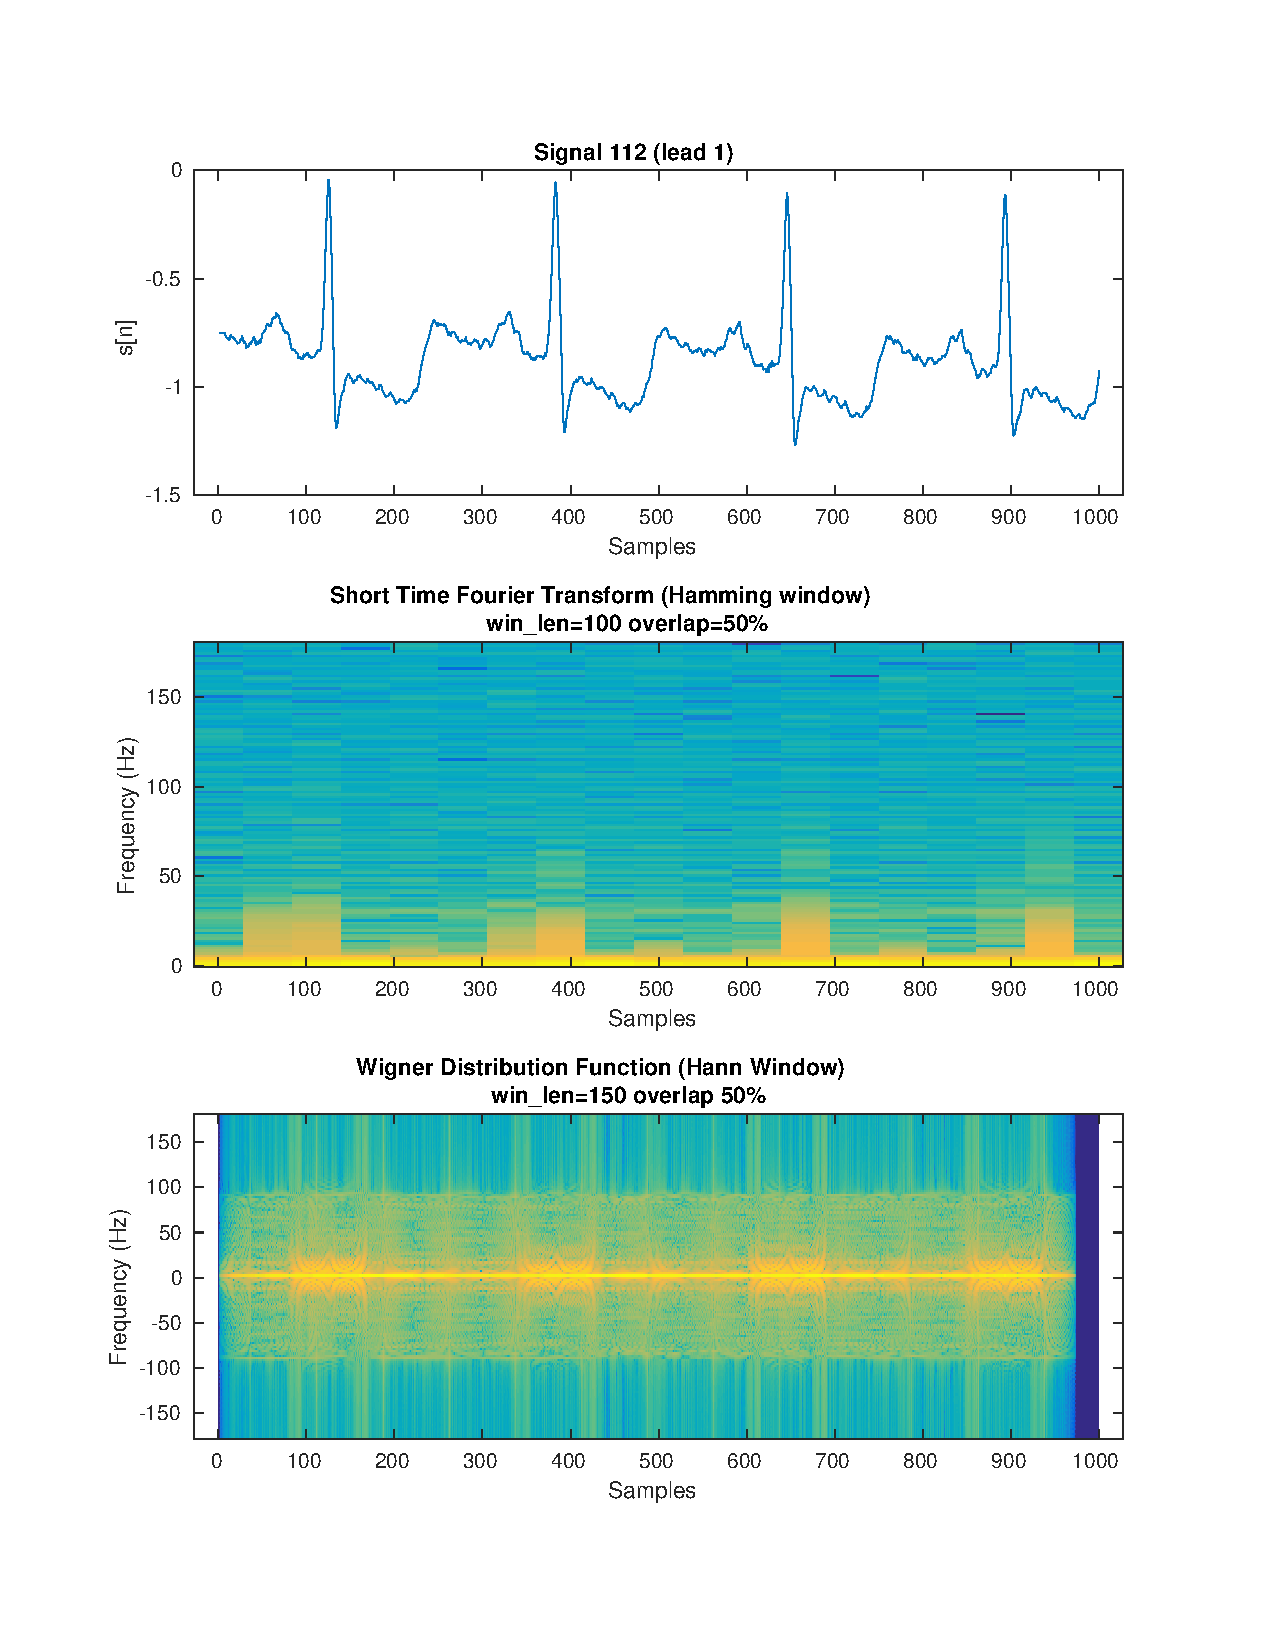
\includegraphics[width=\textwidth]{fig/112l1_stft_wdf.pdf}
\end{minipage}
\begin{minipage}{0.48\textwidth}
	\centering
	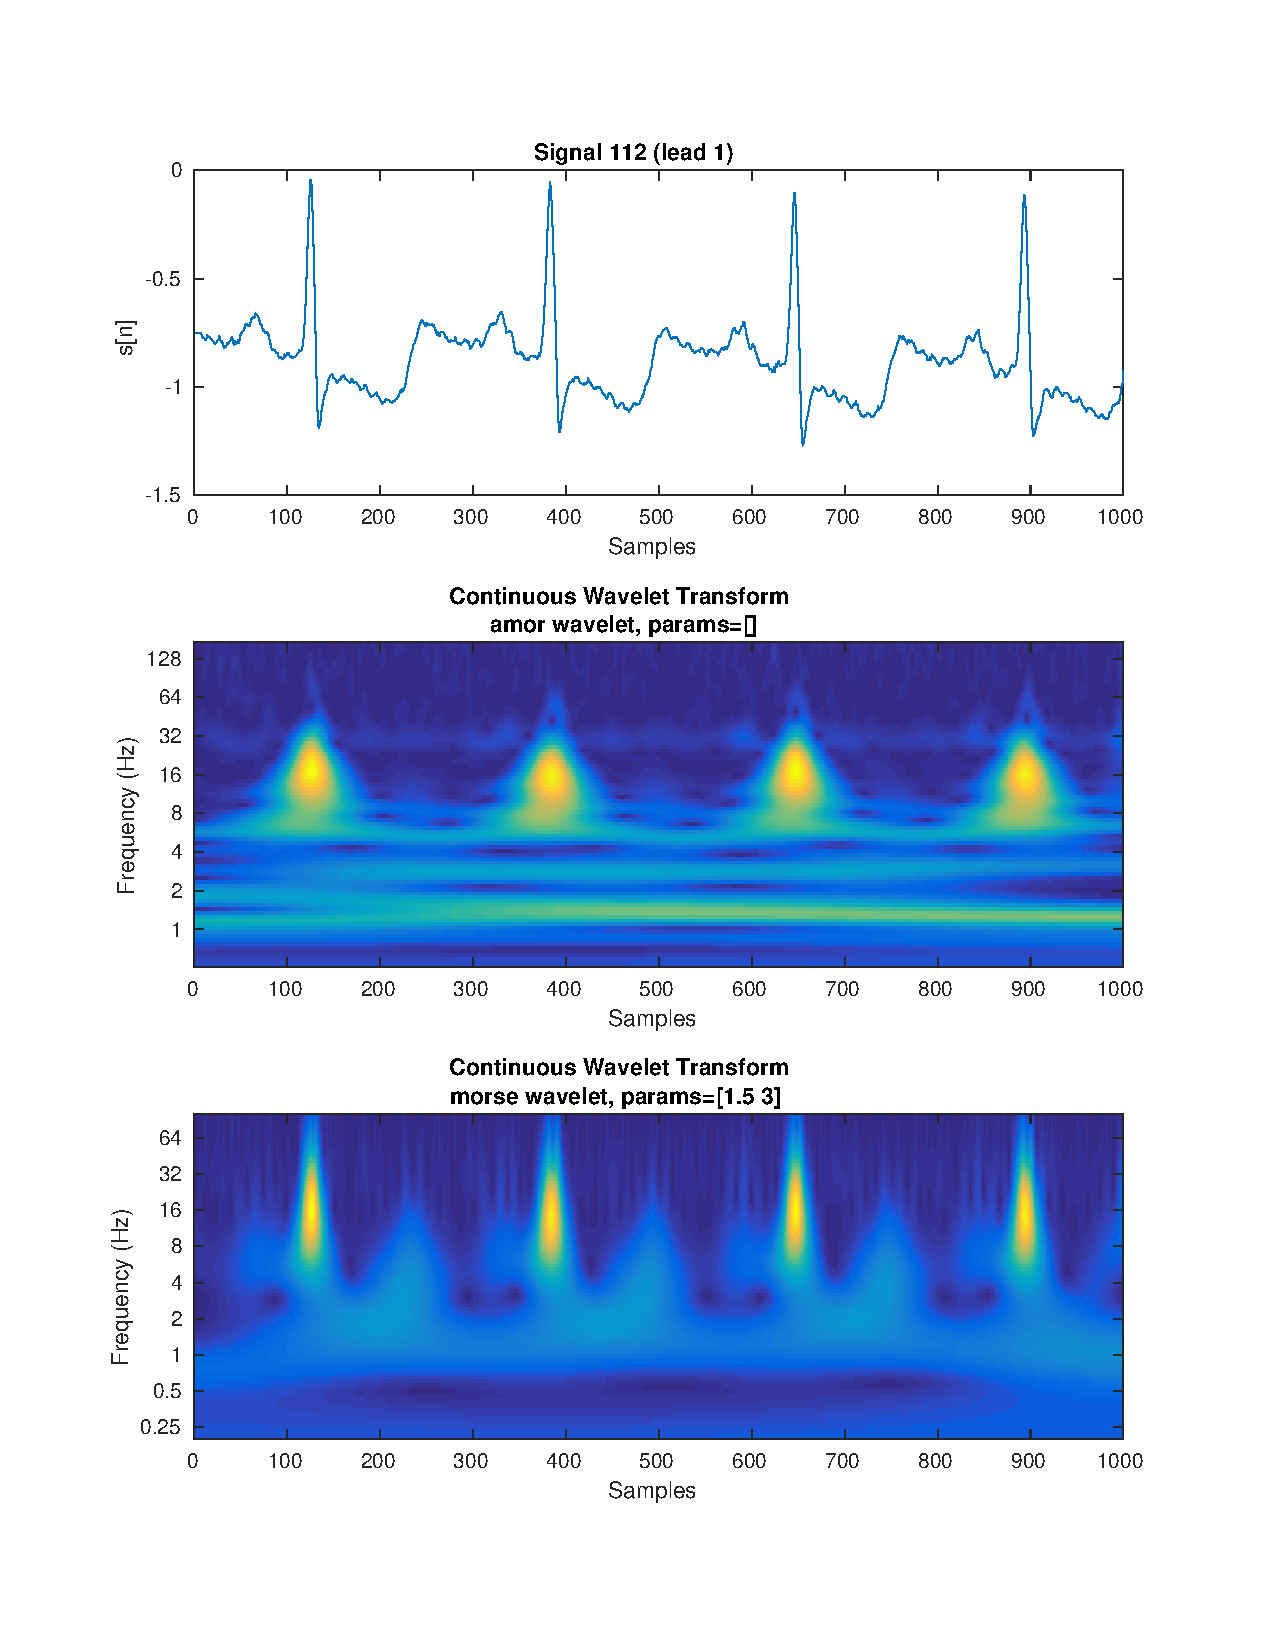
\includegraphics[width=\textwidth]{fig/112l1_cwt.pdf}
\end{minipage}
\vfill
\caption{STFT, WDF και συνεχής WT του σήματος 112. Μπορούμε να διακρίνουμε εύκολα στη συχνότητα τα QRS complexes και τις αργές μεταβολές του σήματος.}
\label{fig:112l1_stft_wdf_wt}
\end{figure}


% --- DWT ---
\begin{figure}[H]
\centering
\begin{minipage}{0.48\textwidth}
	\centering
	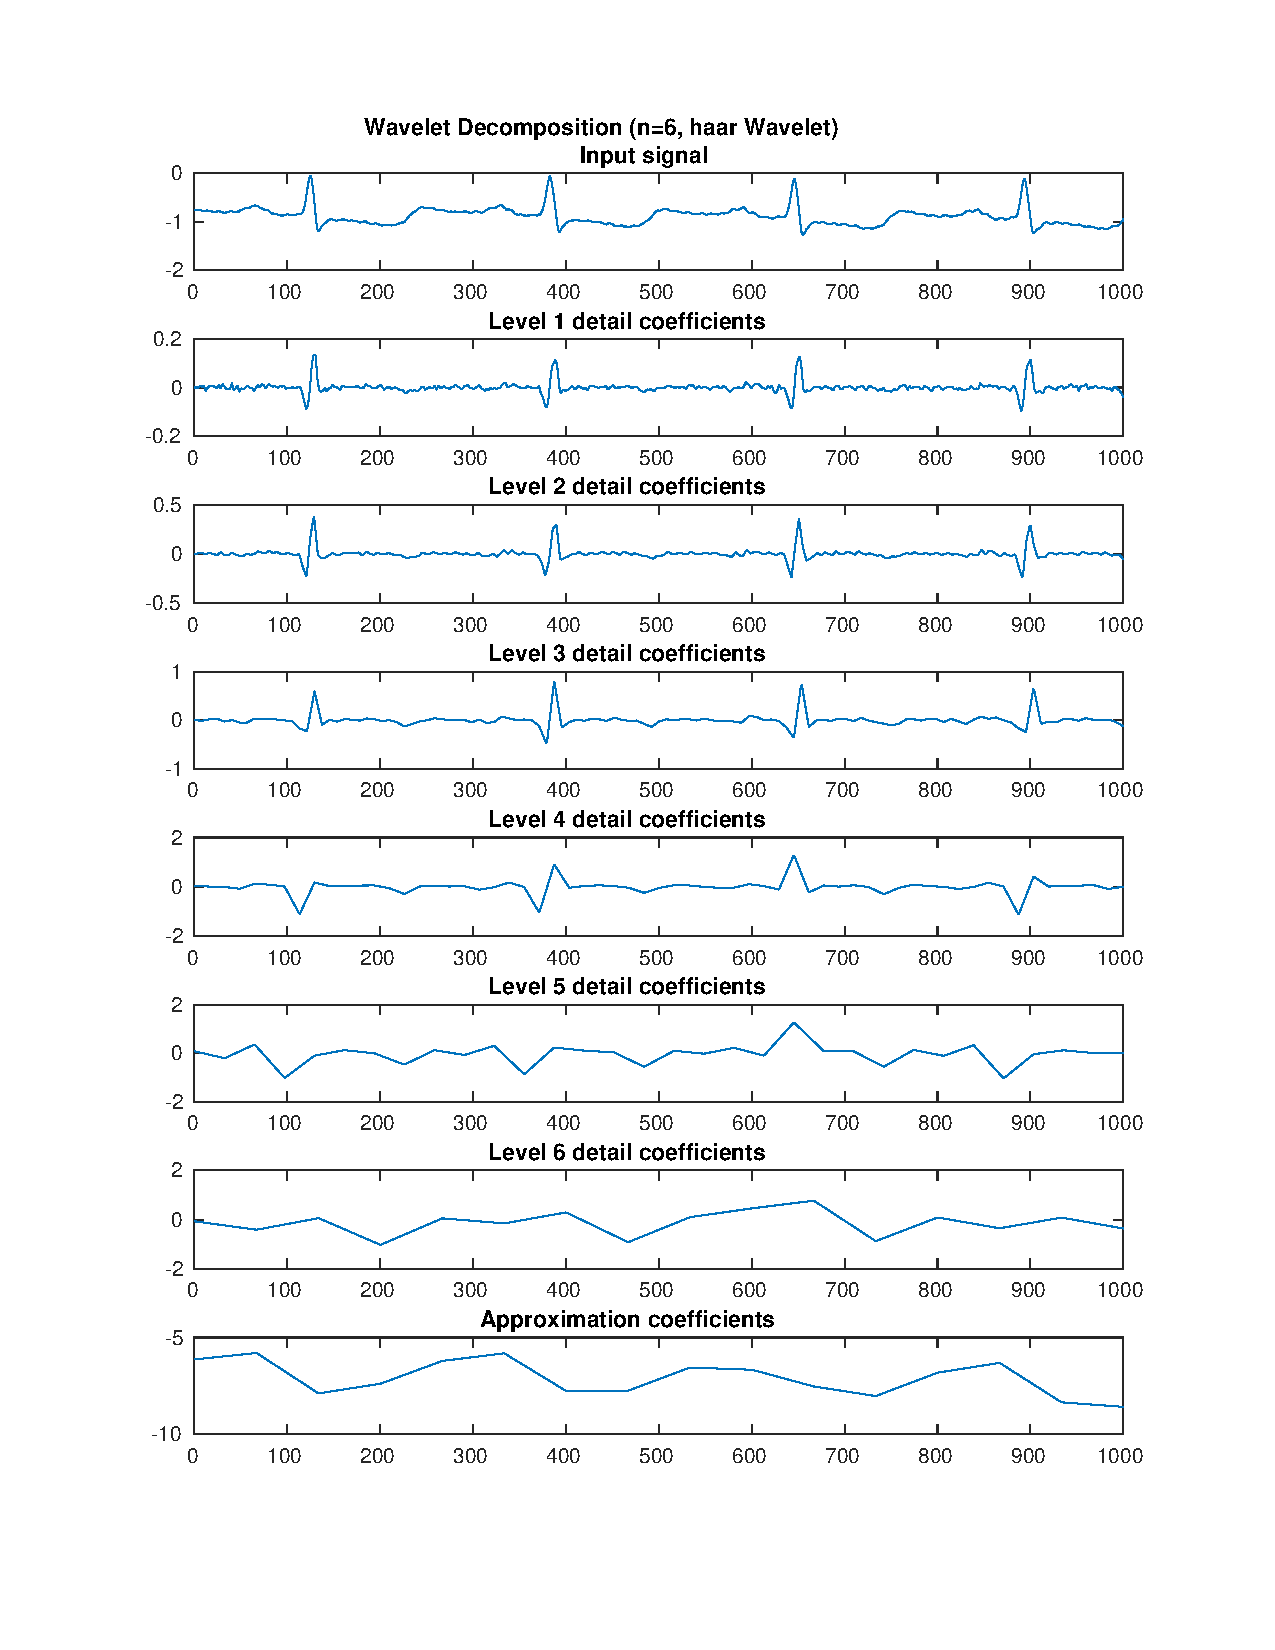
\includegraphics[width=\textwidth]{fig/112l1_dwt1.pdf}
\end{minipage}
\begin{minipage}{0.48\textwidth}
	\centering
	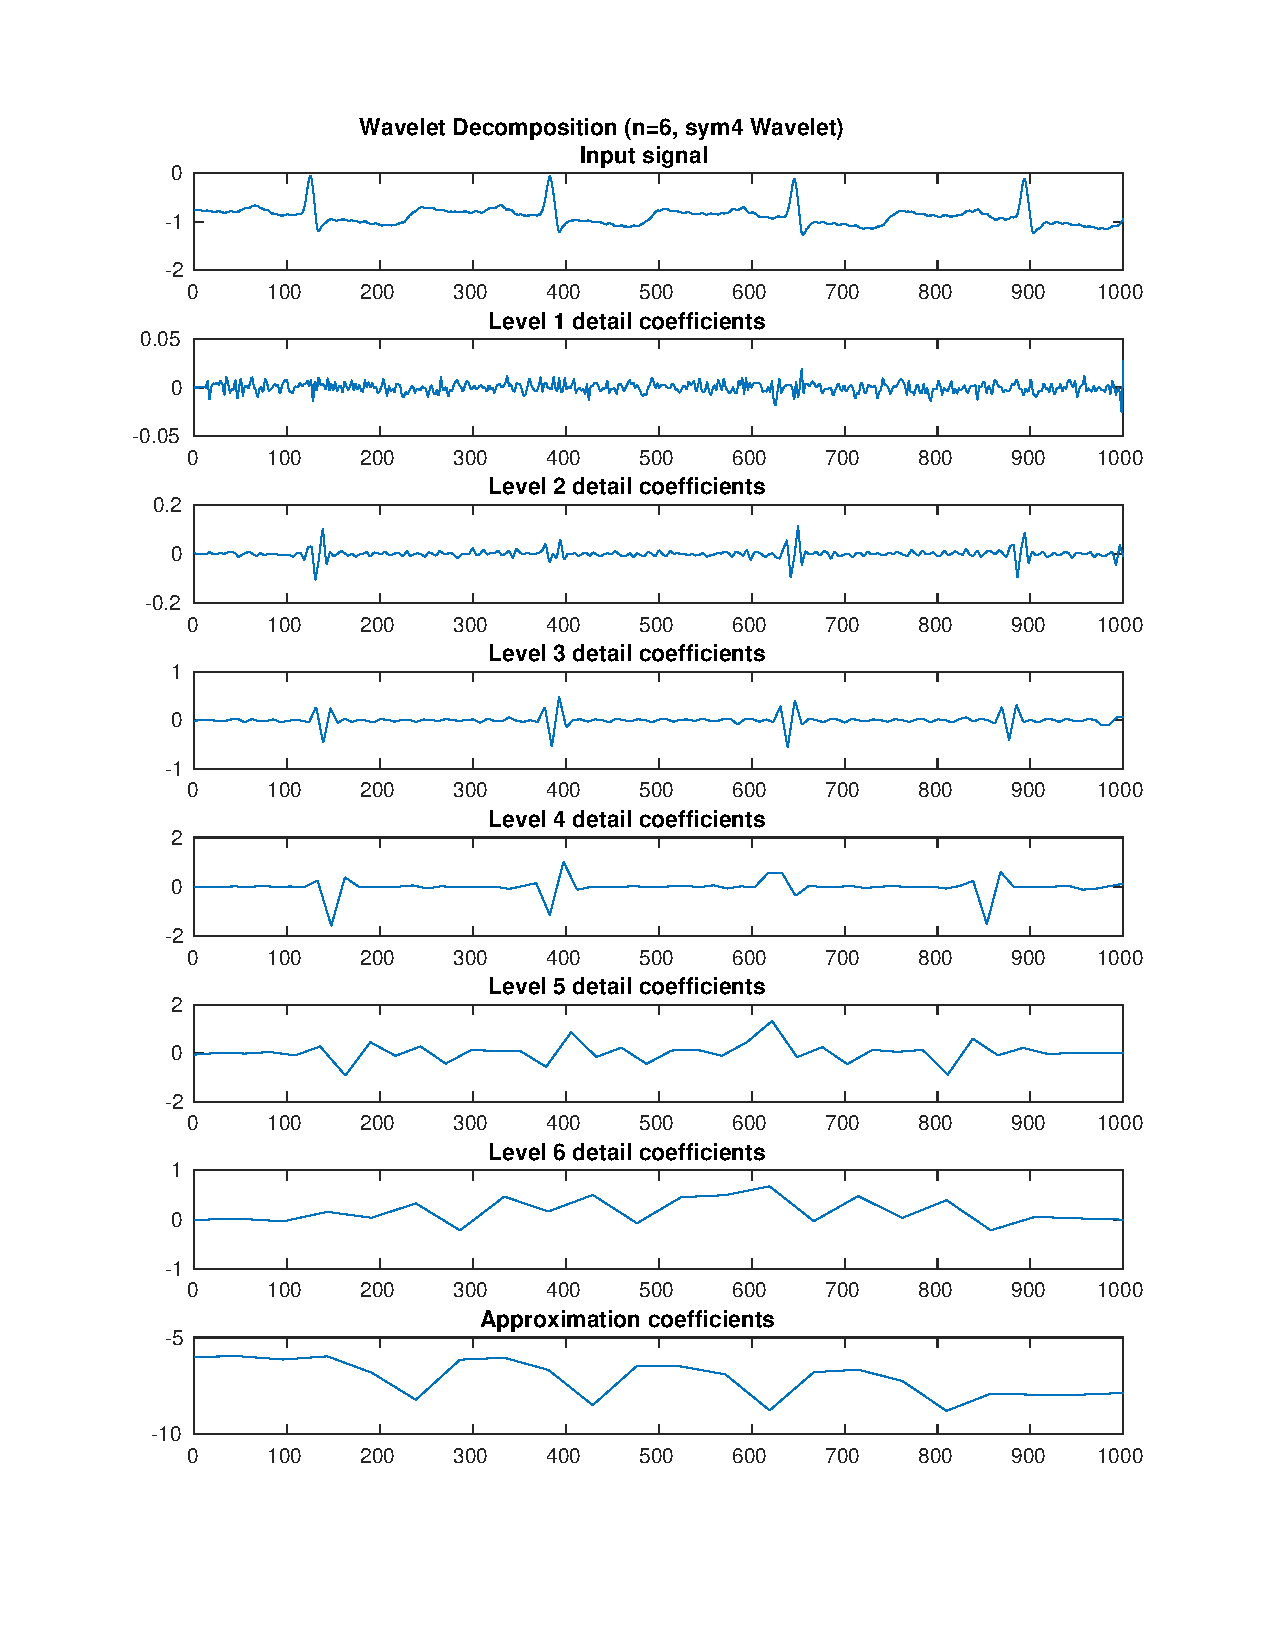
\includegraphics[width=\textwidth]{fig/112l1_dwt2.pdf}
\end{minipage}
\vfill
\caption{Διακριτός WT χρησιμοποιώντας db4 και bior1.3. Τα QRS complexes εμφανίζονται στους συντελεστές των $d_{1-5}$. Εφαρμόστηκε παρεμβολή στους συντελεστές για να είναι ισομεγέθεις.}
\label{fig:112l1_dwt}
\end{figure}


% --- EMD/HHT ---
\begin{figure}[H]
\centering
\begin{minipage}{0.48\textwidth}
	\centering
	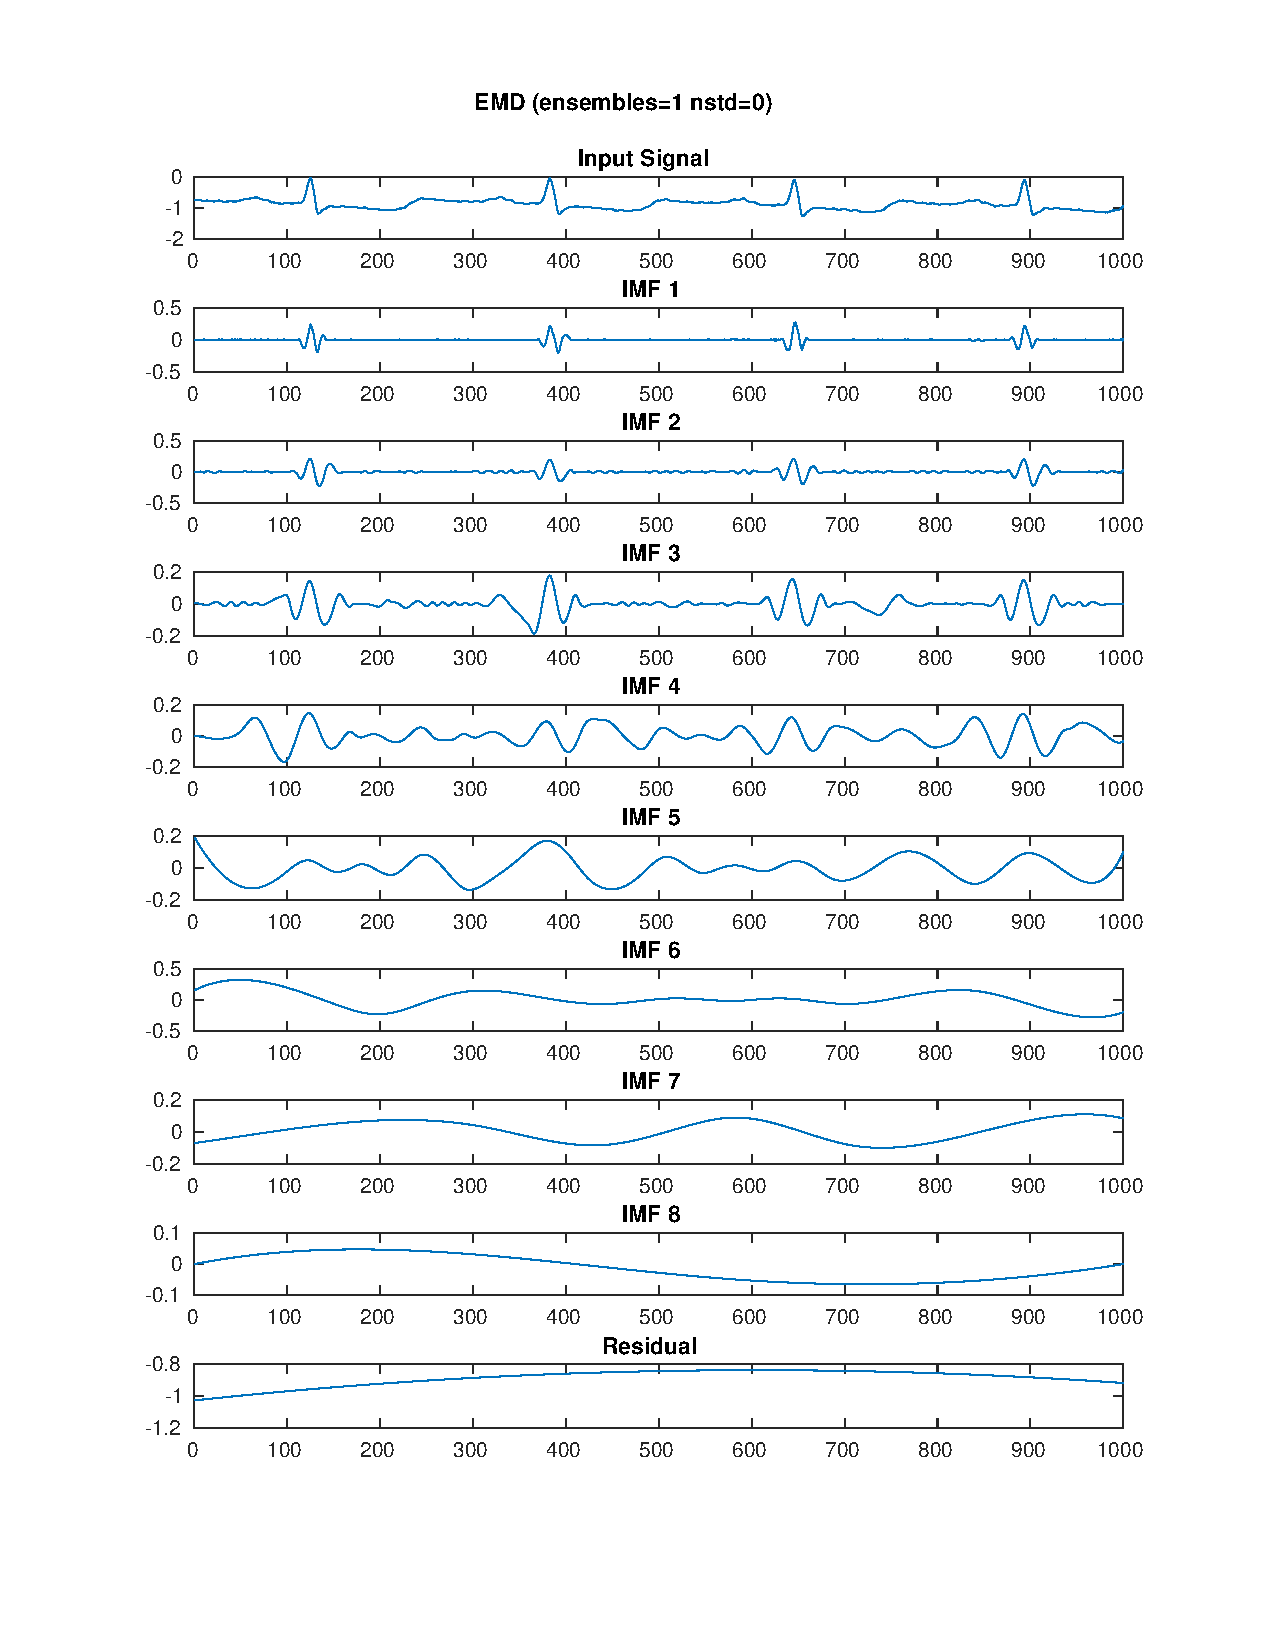
\includegraphics[width=\textwidth]{fig/112l1_emd.pdf}
\end{minipage}
\begin{minipage}{0.48\textwidth}
	\centering
	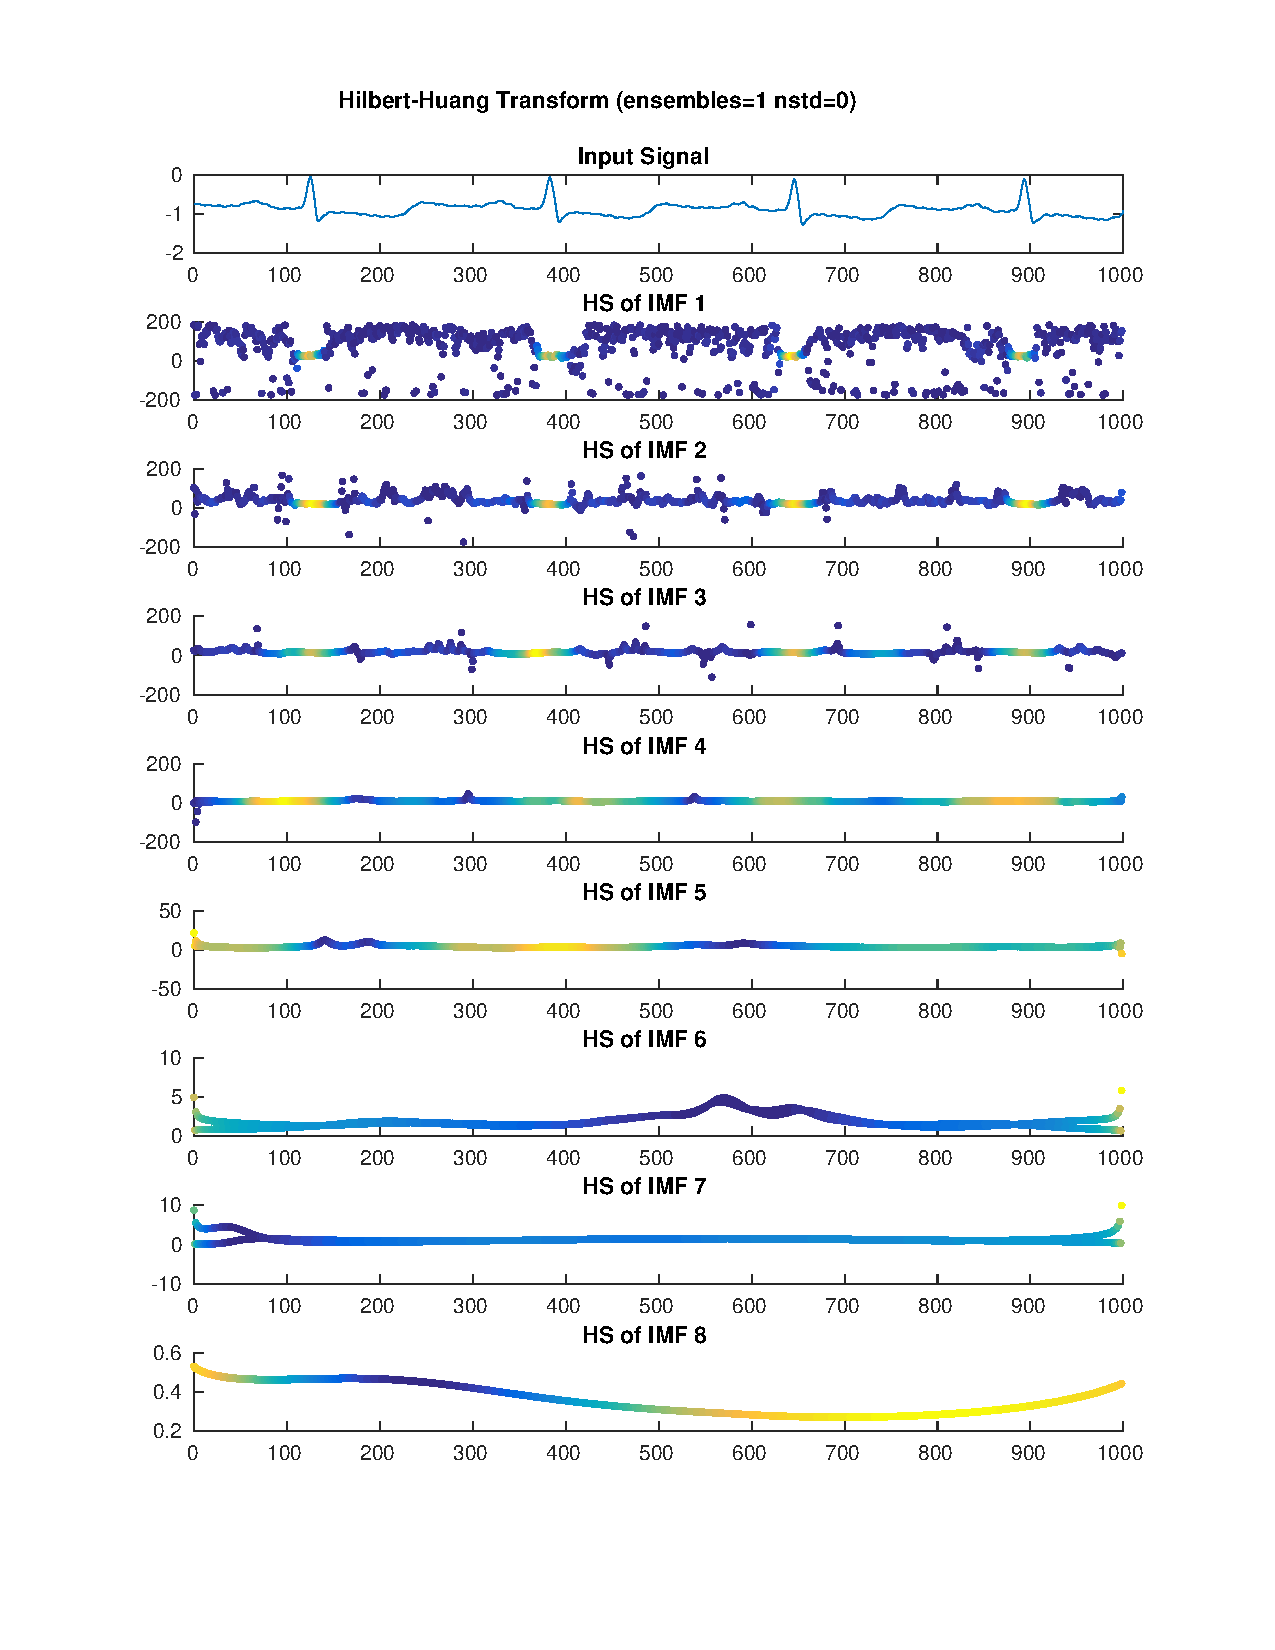
\includegraphics[width=\textwidth]{fig/112l1_hht.pdf}
\end{minipage}
\vfill
\caption{EMD και HHT του σήματος 112. Στα $IMF_{2-3}$ περιέχονται τα QRS complexes, στο $IMF_{6}$ περιγράφεται ο καρδιακός ρυθμός.}
\label{fig:112l1_hht}
\end{figure}


% --- EEMD/HHT ---
\begin{figure}[H]
\centering
\begin{minipage}{0.48\textwidth}
	\centering
	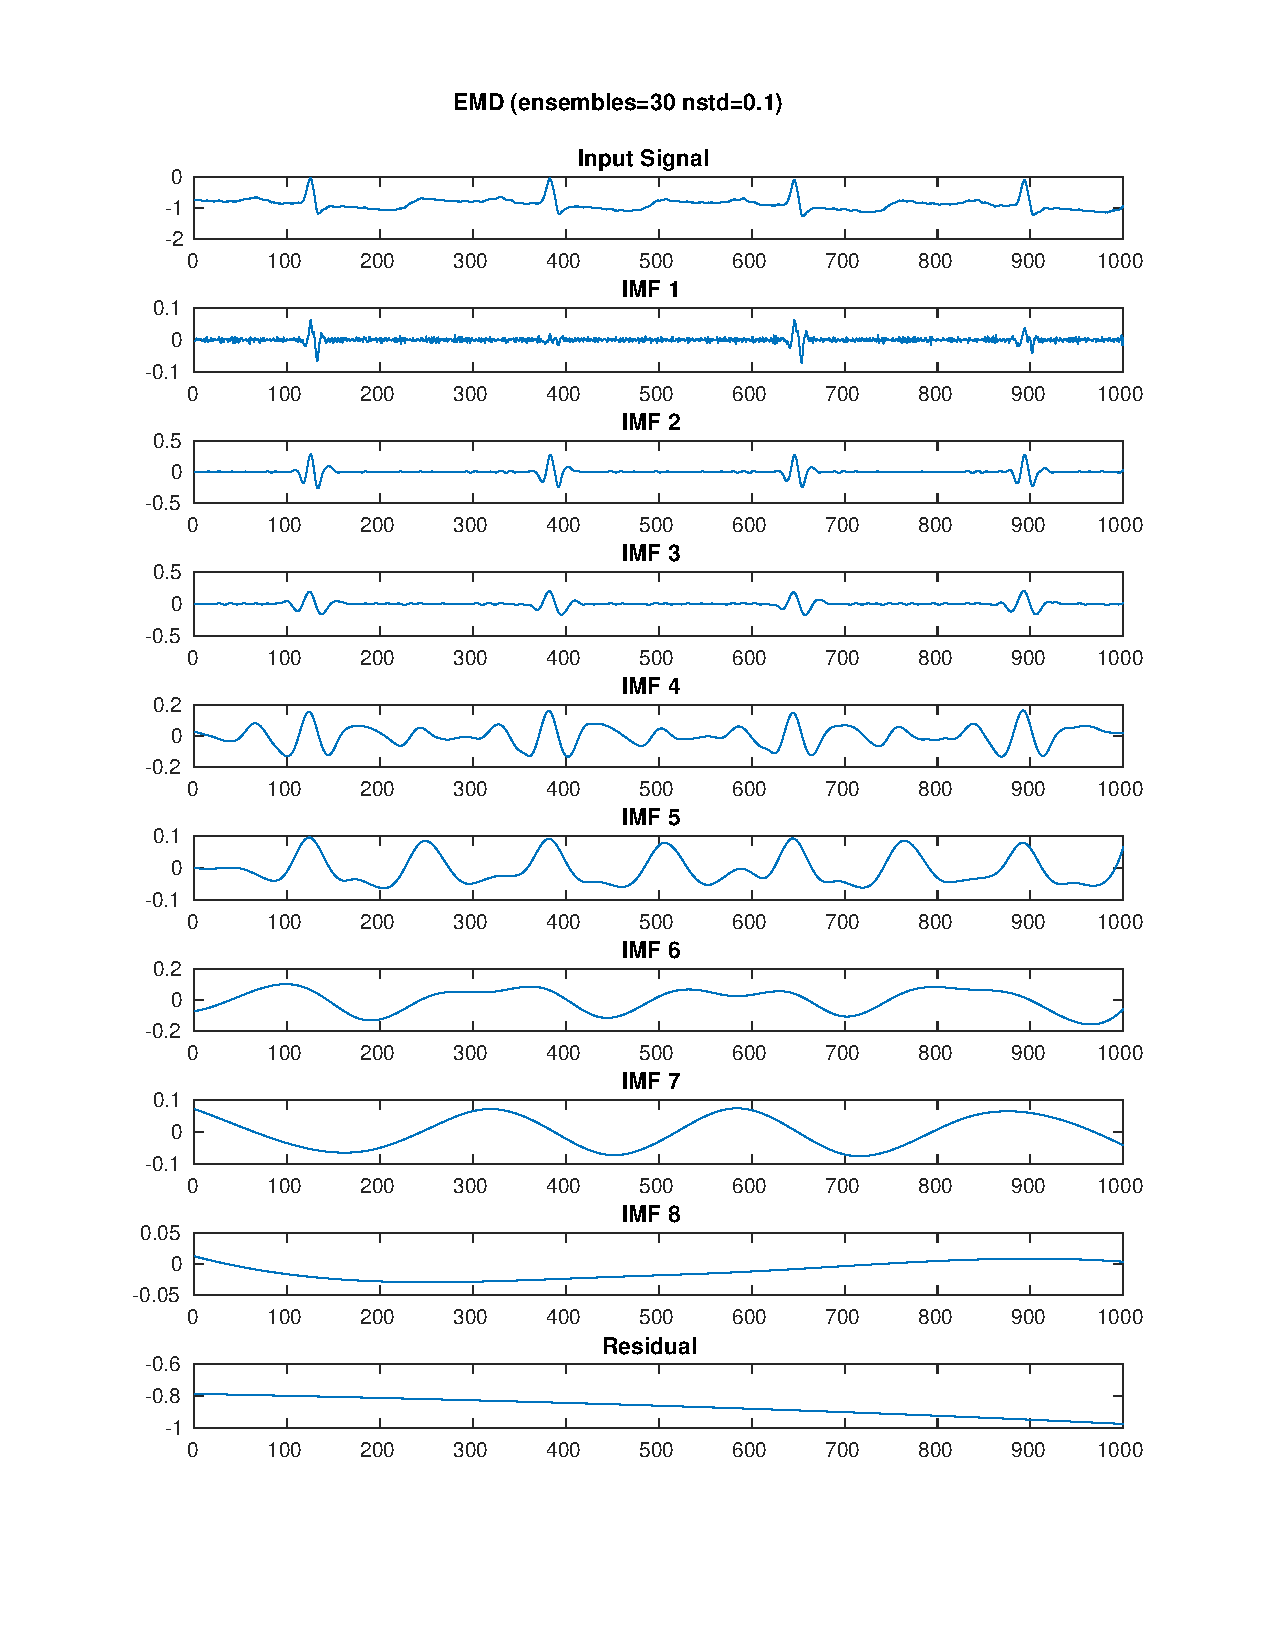
\includegraphics[width=\textwidth]{fig/112l1_emd_ensemble.pdf}
\end{minipage}
\begin{minipage}{0.48\textwidth}
	\centering
	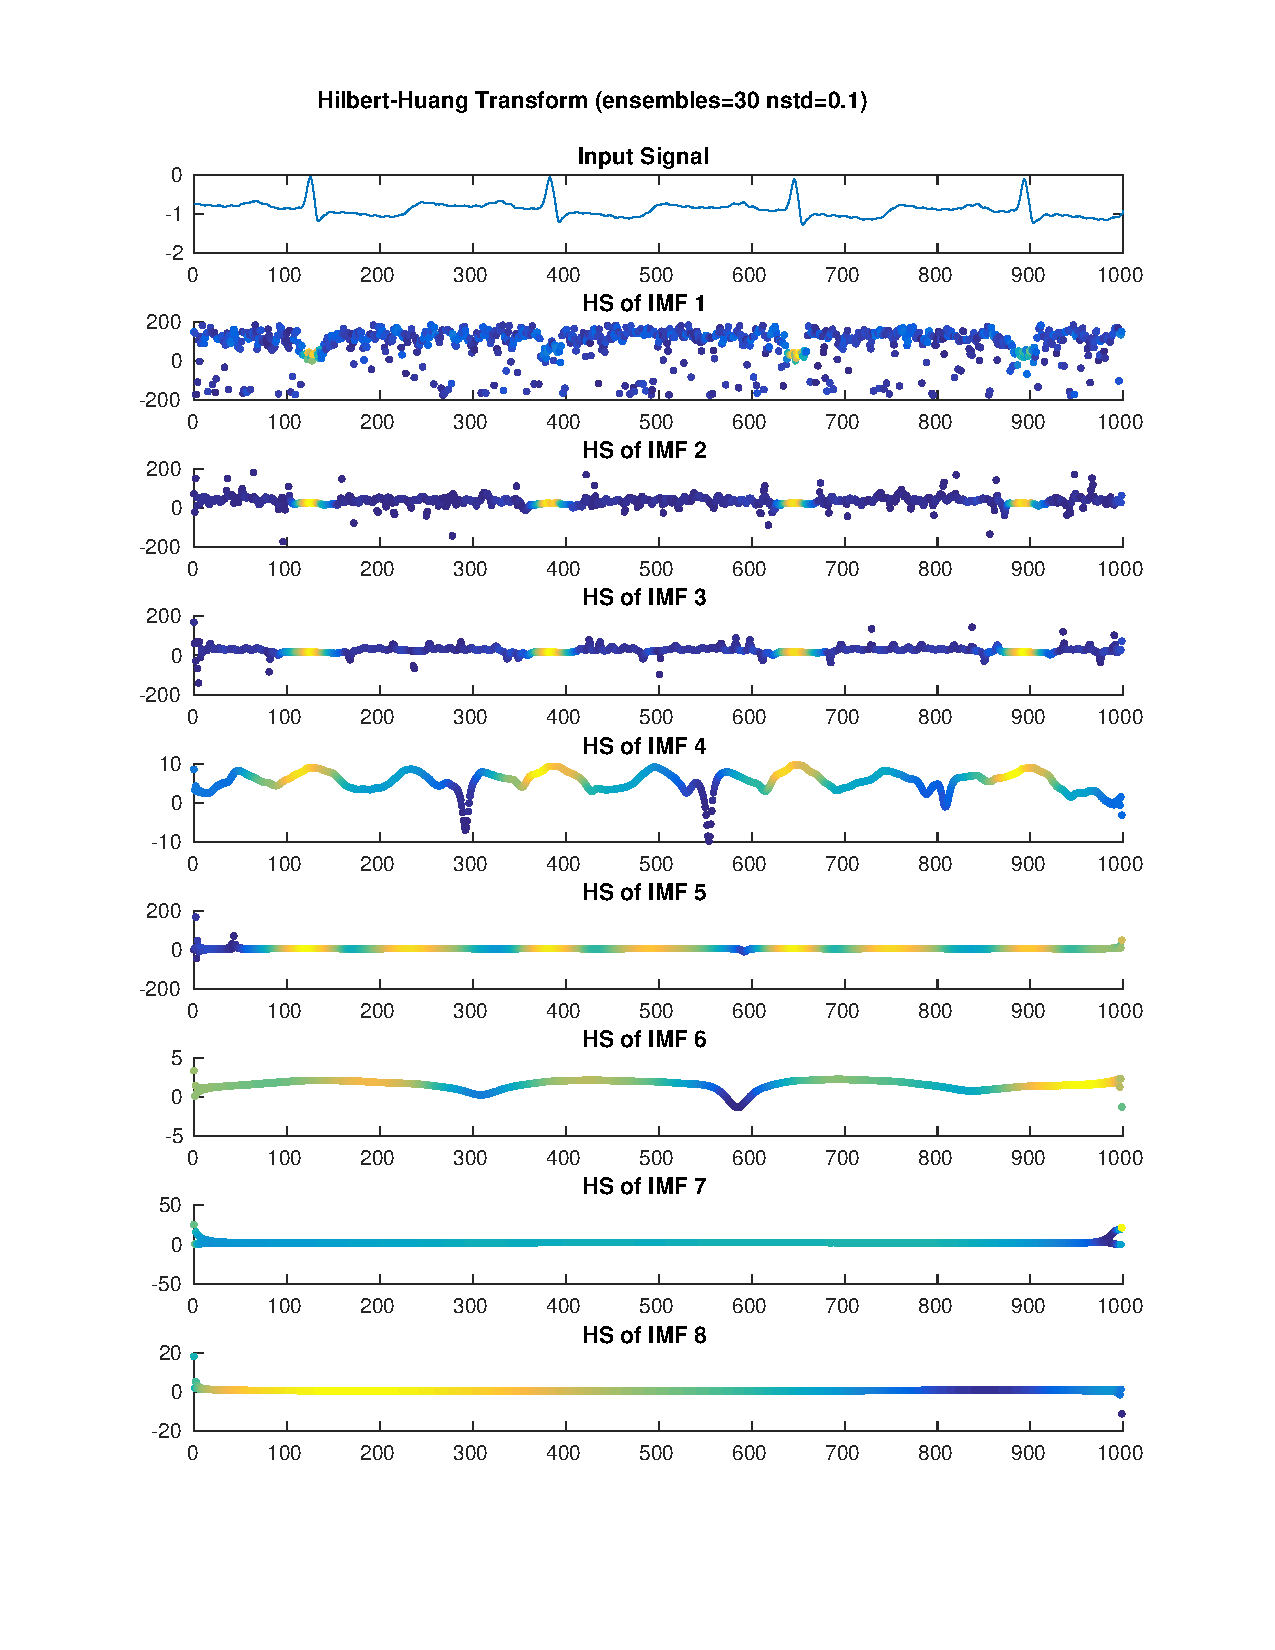
\includegraphics[width=\textwidth]{fig/112l1_hht_ensemble.pdf}
\end{minipage}
\vfill
\caption{EEMD και HHT του σήματος 112, με $n_{ens}=100$ και $\sigma_n = 0.1$. Το mode mixing μεταξύ των IMFs έχει μειωθεί σε σύγκριση με τον απλό EMD. Ο καρδιακός παλμός του $IMF_{7}$ είναι πιο σταθερός.}
\label{fig:112l1_hht_ensemble}
\end{figure}

\subsubsection*{Σήμα 112 (Ακροδέκτης 2)}

% --- STFT, WDF, CWT ---
\begin{figure}[H]
\centering
\begin{minipage}{0.48\textwidth}
	\centering
	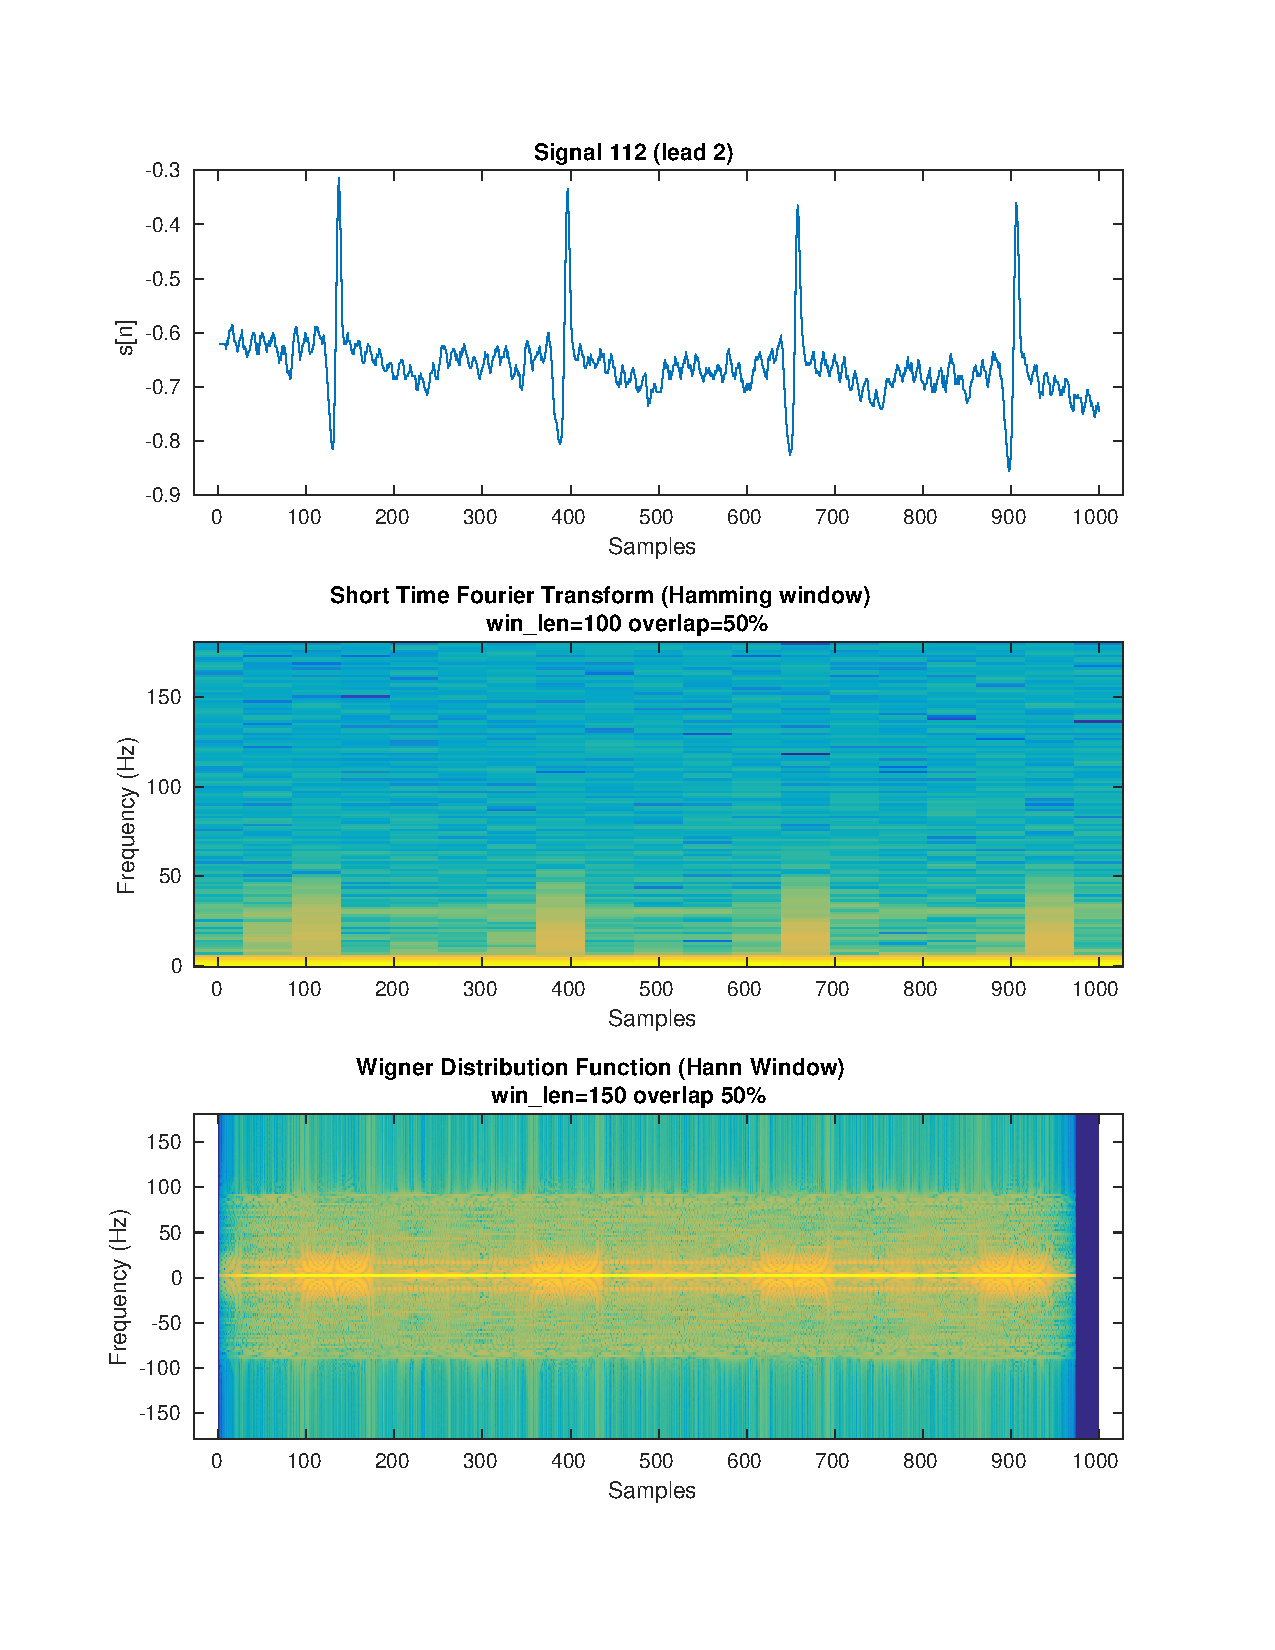
\includegraphics[width=\textwidth]{fig/112l2_stft_wdf.pdf}
\end{minipage}
\begin{minipage}{0.48\textwidth}
	\centering
	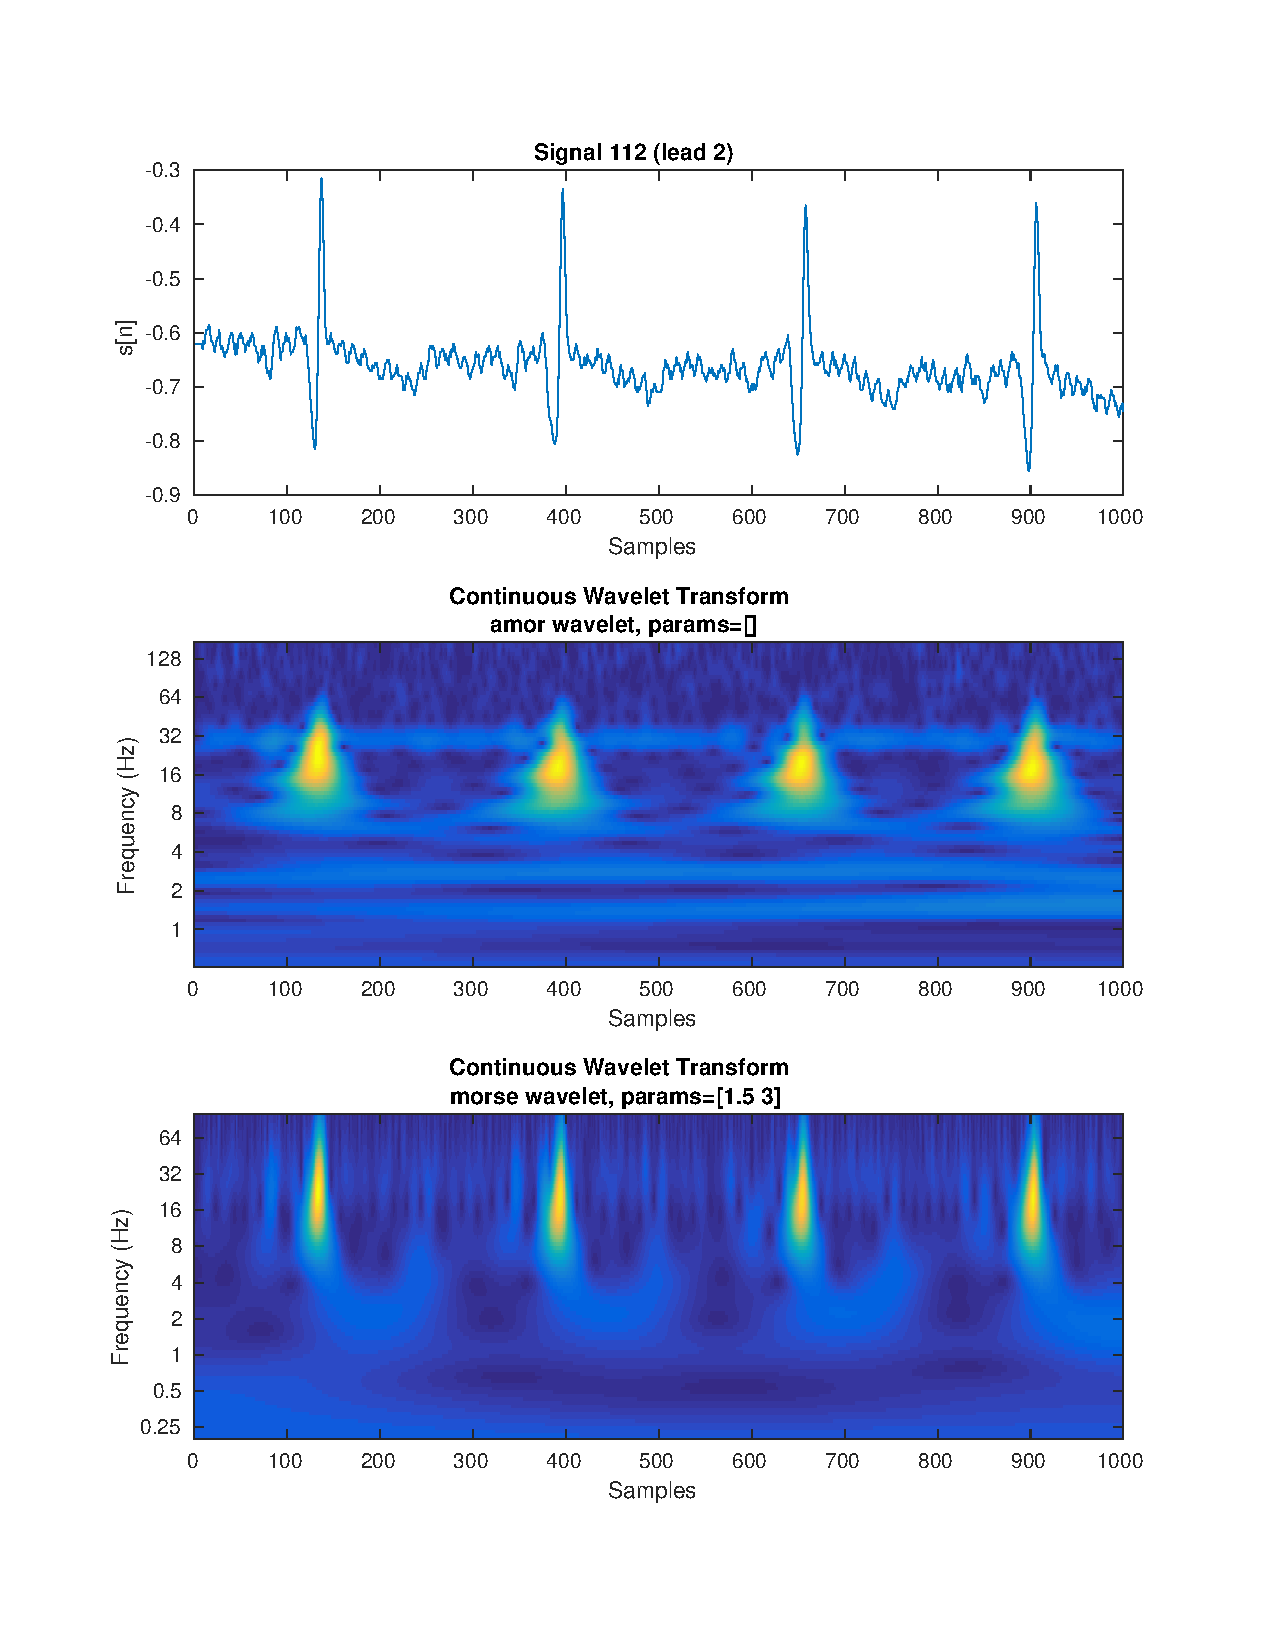
\includegraphics[width=\textwidth]{fig/112l2_cwt.pdf}
\end{minipage}
\vfill
\caption{STFT, WDF και συνεχής WT του σήματος 112 (ακροδέκτης 2). Τα αποτελέσματα συμφωνούν με την περίπτωση του ακροδέκτη 1, με μόνη διαφορά ότι εμφανίζεται ισχυρότερος ο θόρυβος αναπαραγωγής στα 30Hz.}
\label{fig:112l2_stft_wdf_wt}
\end{figure}


% --- DWT ---
\begin{figure}[H]
\centering
\begin{minipage}{0.48\textwidth}
	\centering
	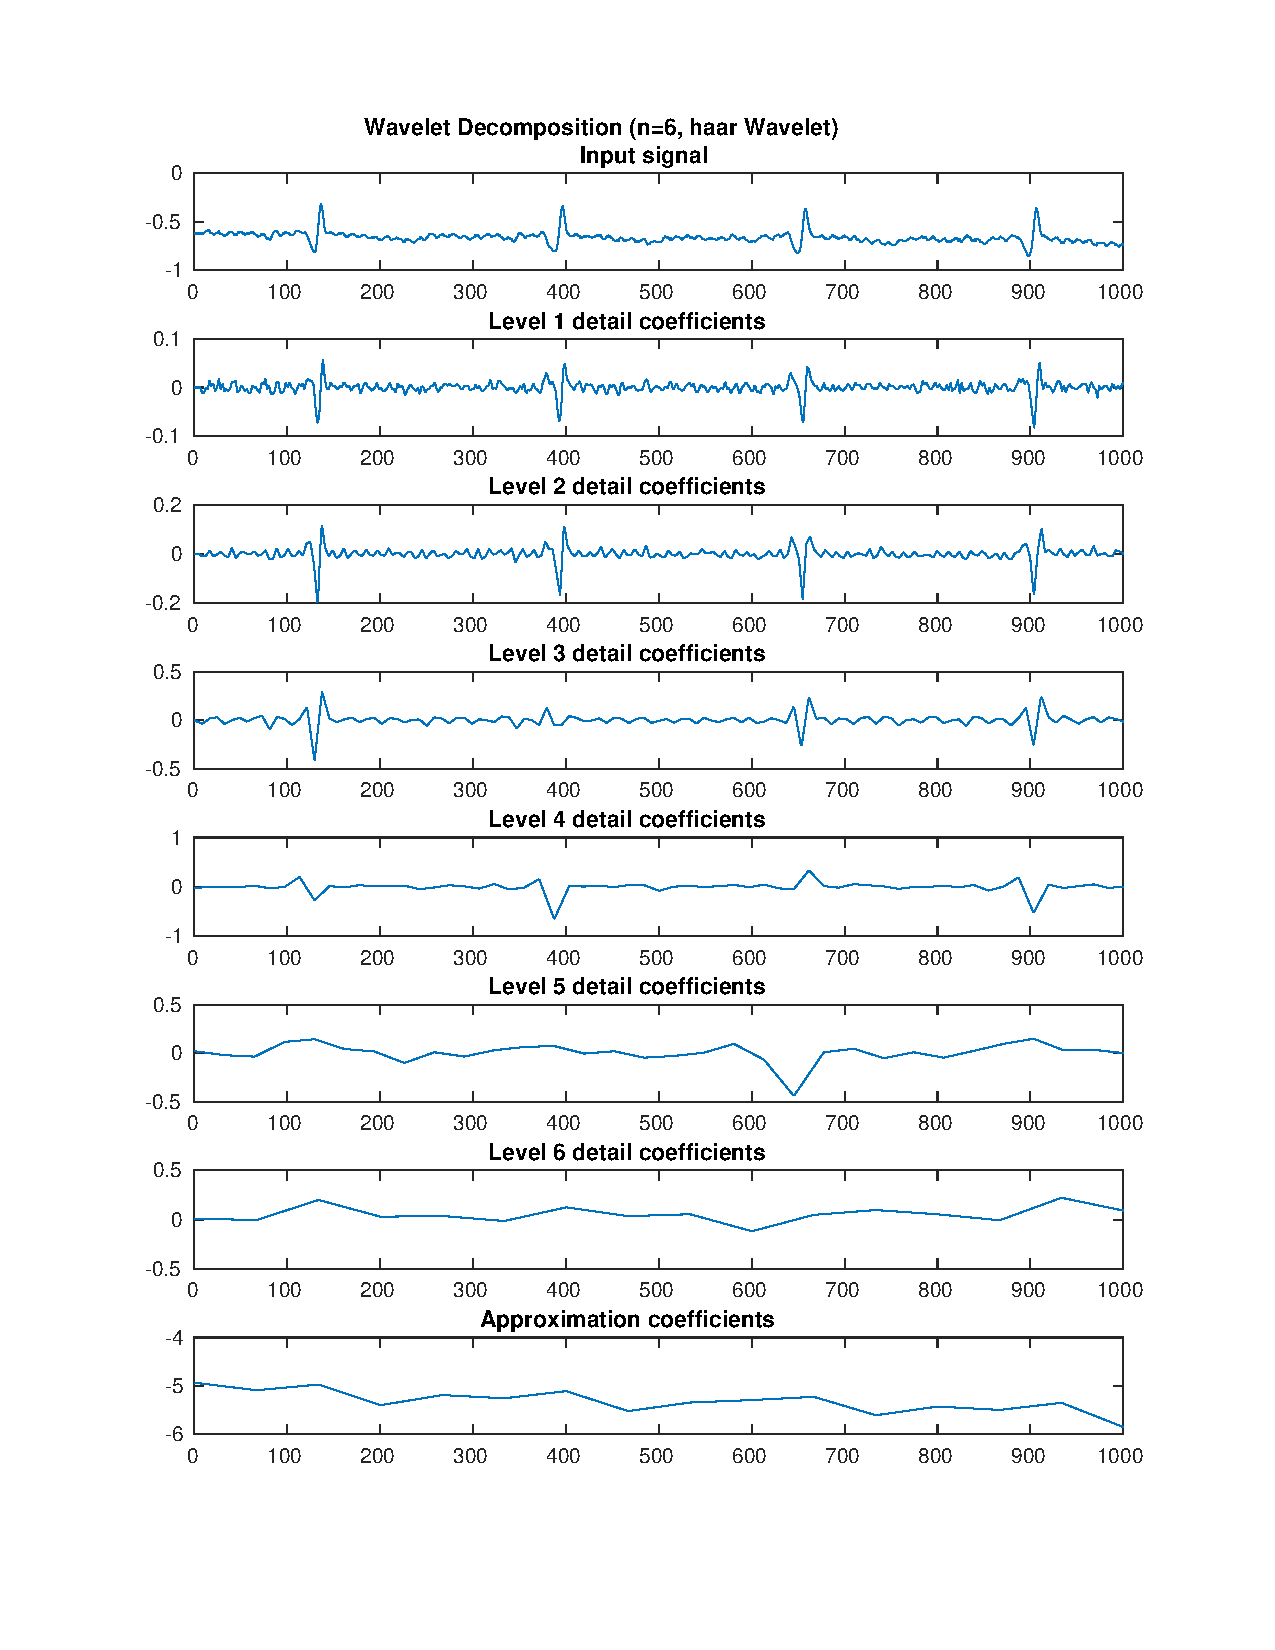
\includegraphics[width=\textwidth]{fig/112l2_dwt1.pdf}
\end{minipage}
\begin{minipage}{0.48\textwidth}
	\centering
	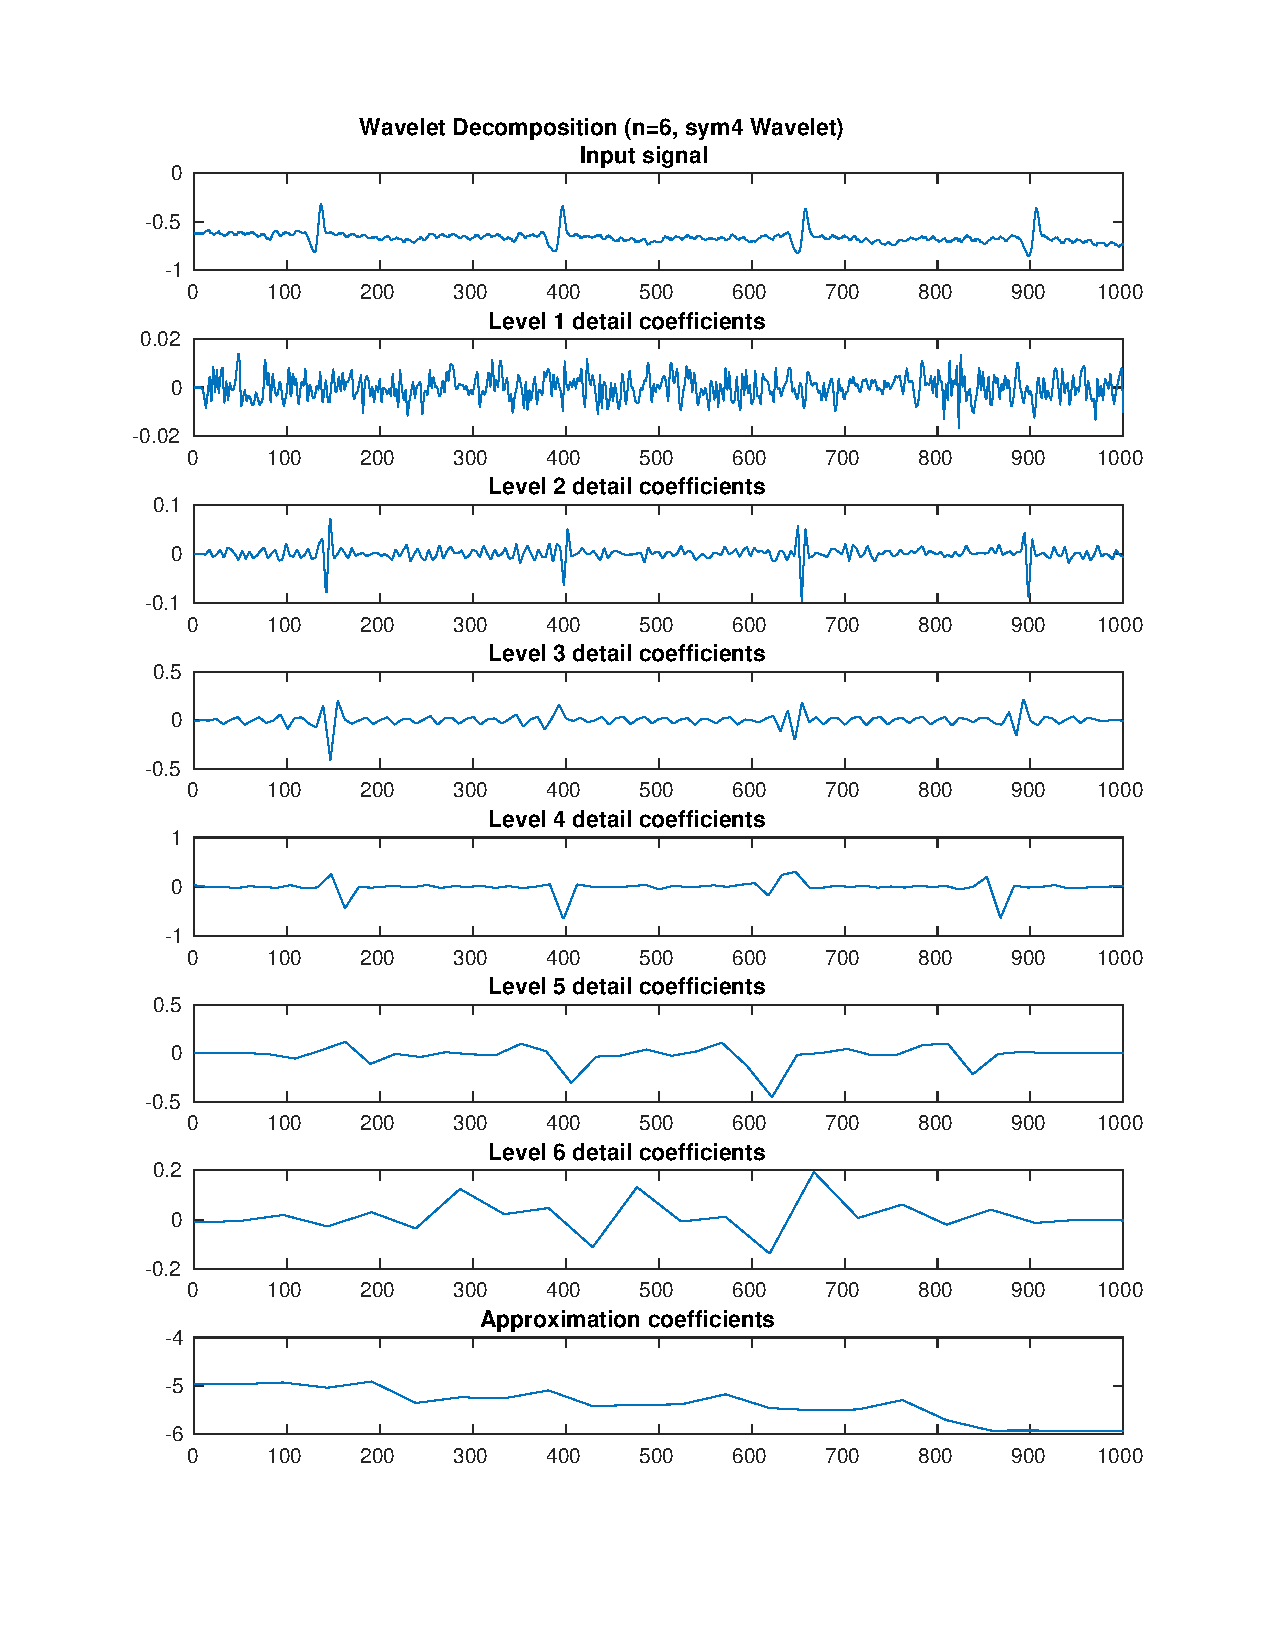
\includegraphics[width=\textwidth]{fig/112l2_dwt2.pdf}
\end{minipage}
\vfill
\caption{Διακριτός WT χρησιμοποιώντας db4 και bior1.3.}
\label{fig:112l2_dwt}
\end{figure}


% --- EMD/HHT ---
\begin{figure}[H]
\centering
\begin{minipage}{0.48\textwidth}
	\centering
	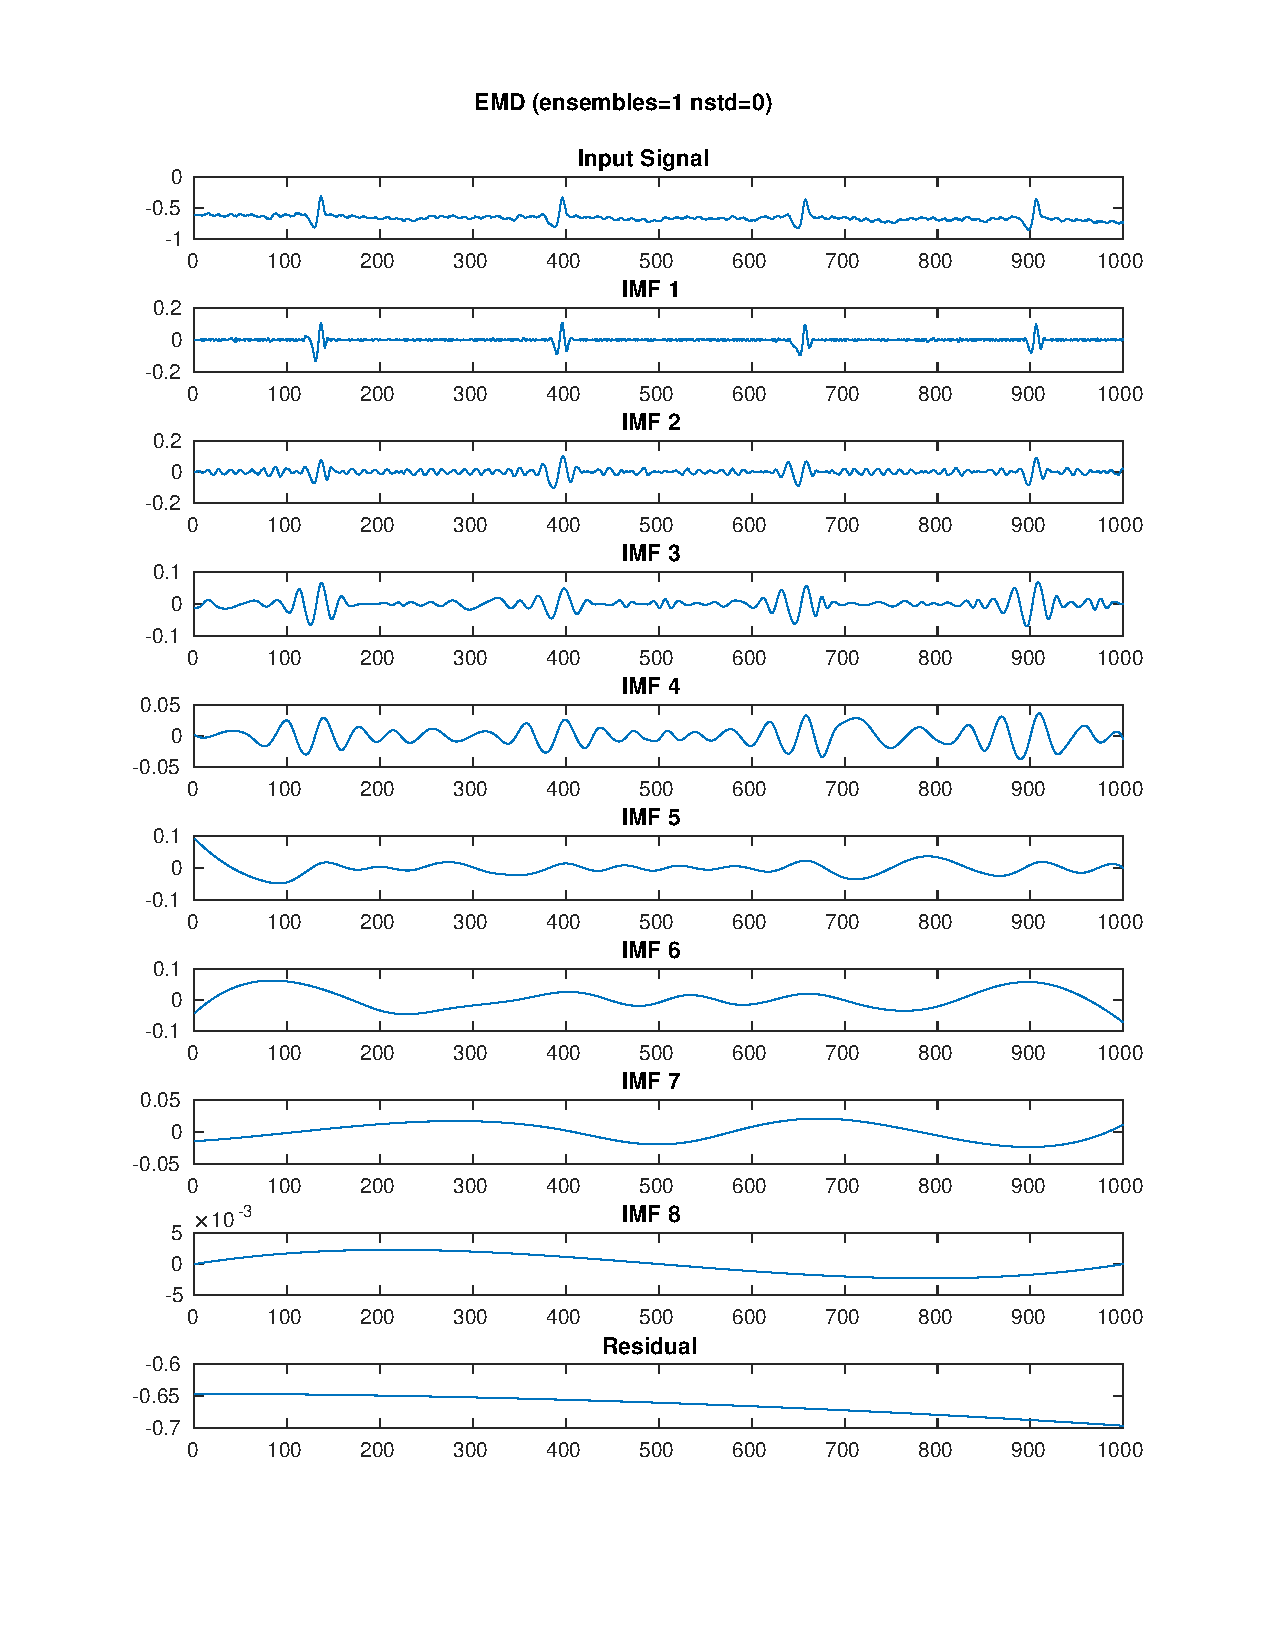
\includegraphics[width=\textwidth]{fig/112l2_emd.pdf}
	
	(α)
\end{minipage}
\begin{minipage}{0.48\textwidth}
	\centering
	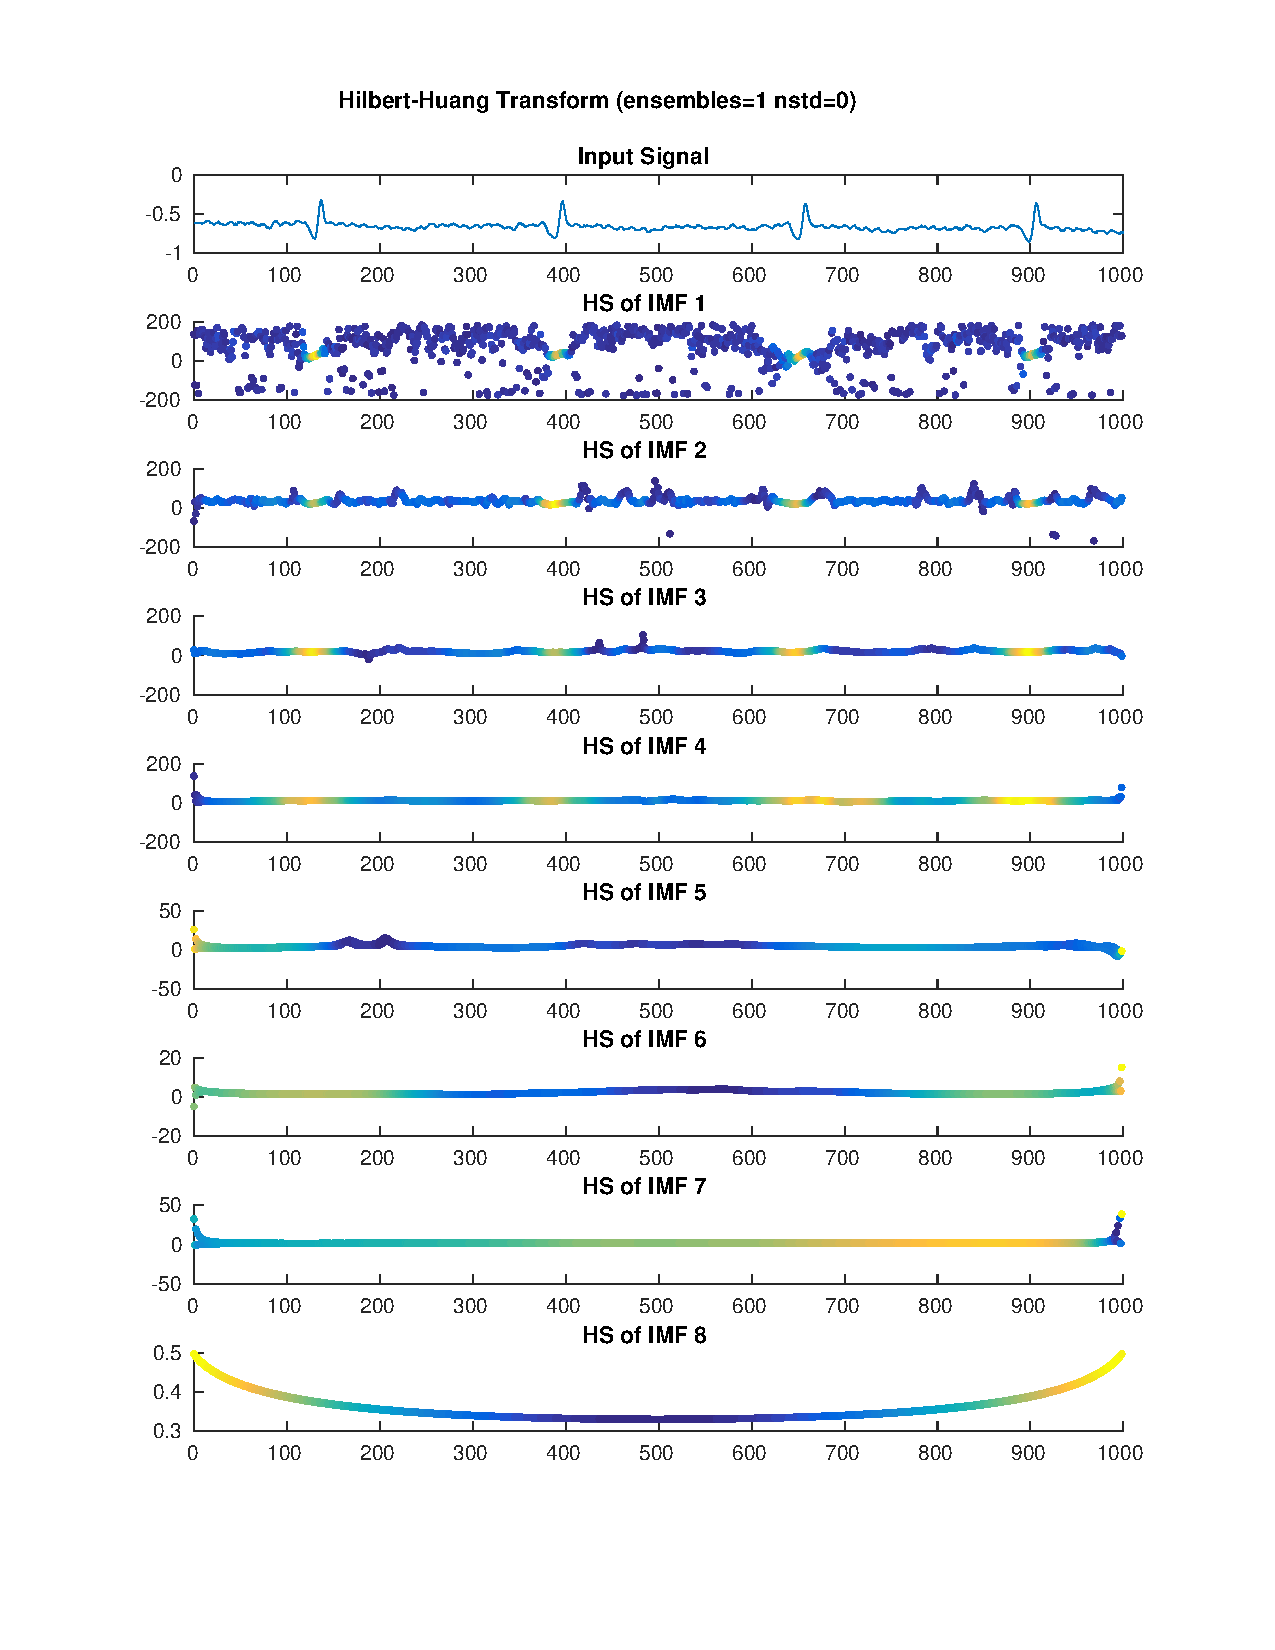
\includegraphics[width=\textwidth]{fig/112l2_hht.pdf}
	
	(β)
\end{minipage}
\vfill
\caption{EMD και HHT του σήματος 112 (ακροδέκτης 2). Τα παραγόμενα IMFs εμφανίζουν εντονότερο mode mixing σε σύγκριση με τον ακροδέκτη 1, πιθανώς λόγω του ισχυρότερου θορύβου.}
\label{fig:112l2_hht}
\end{figure}


% --- EEMD/HHT ---
\begin{figure}[H]
\centering
\begin{minipage}{0.48\textwidth}
	\centering
	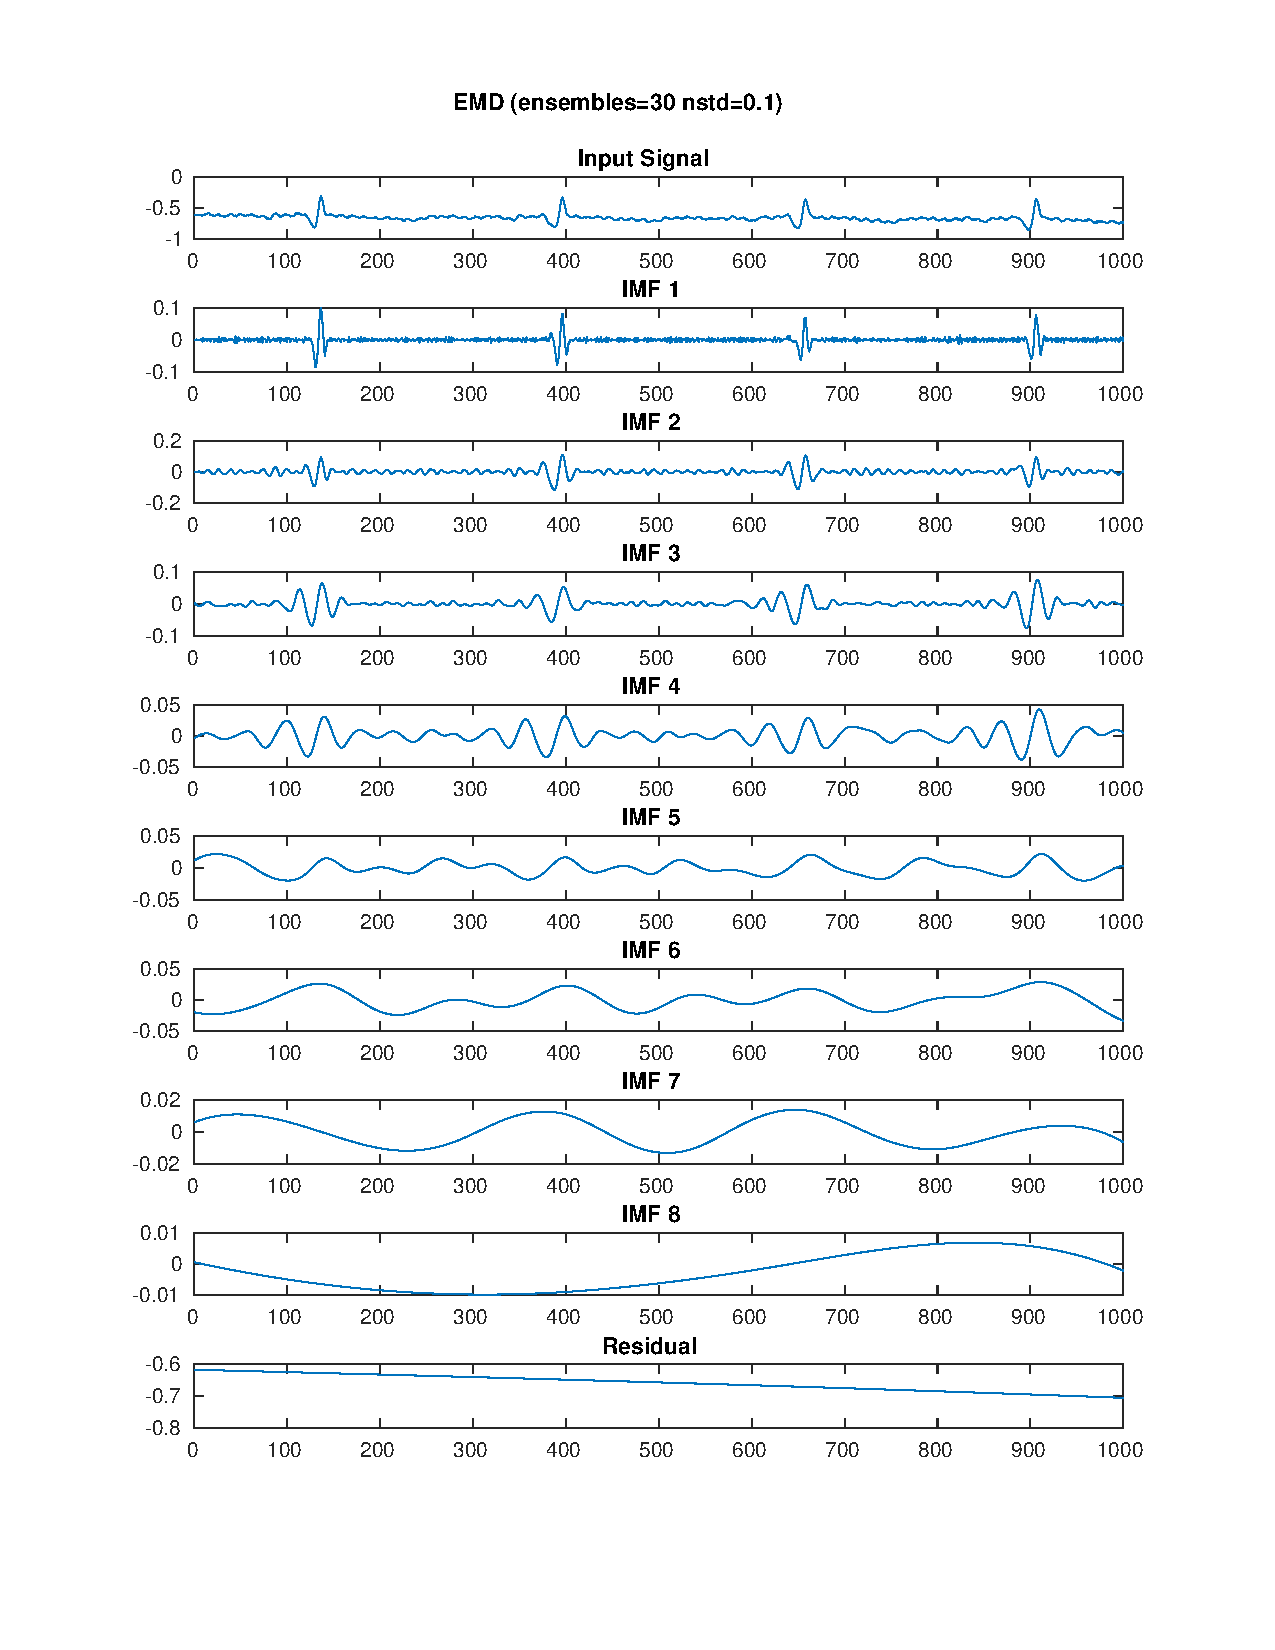
\includegraphics[width=\textwidth]{fig/112l2_emd_ensemble.pdf}
\end{minipage}
\begin{minipage}{0.48\textwidth}
	\centering
	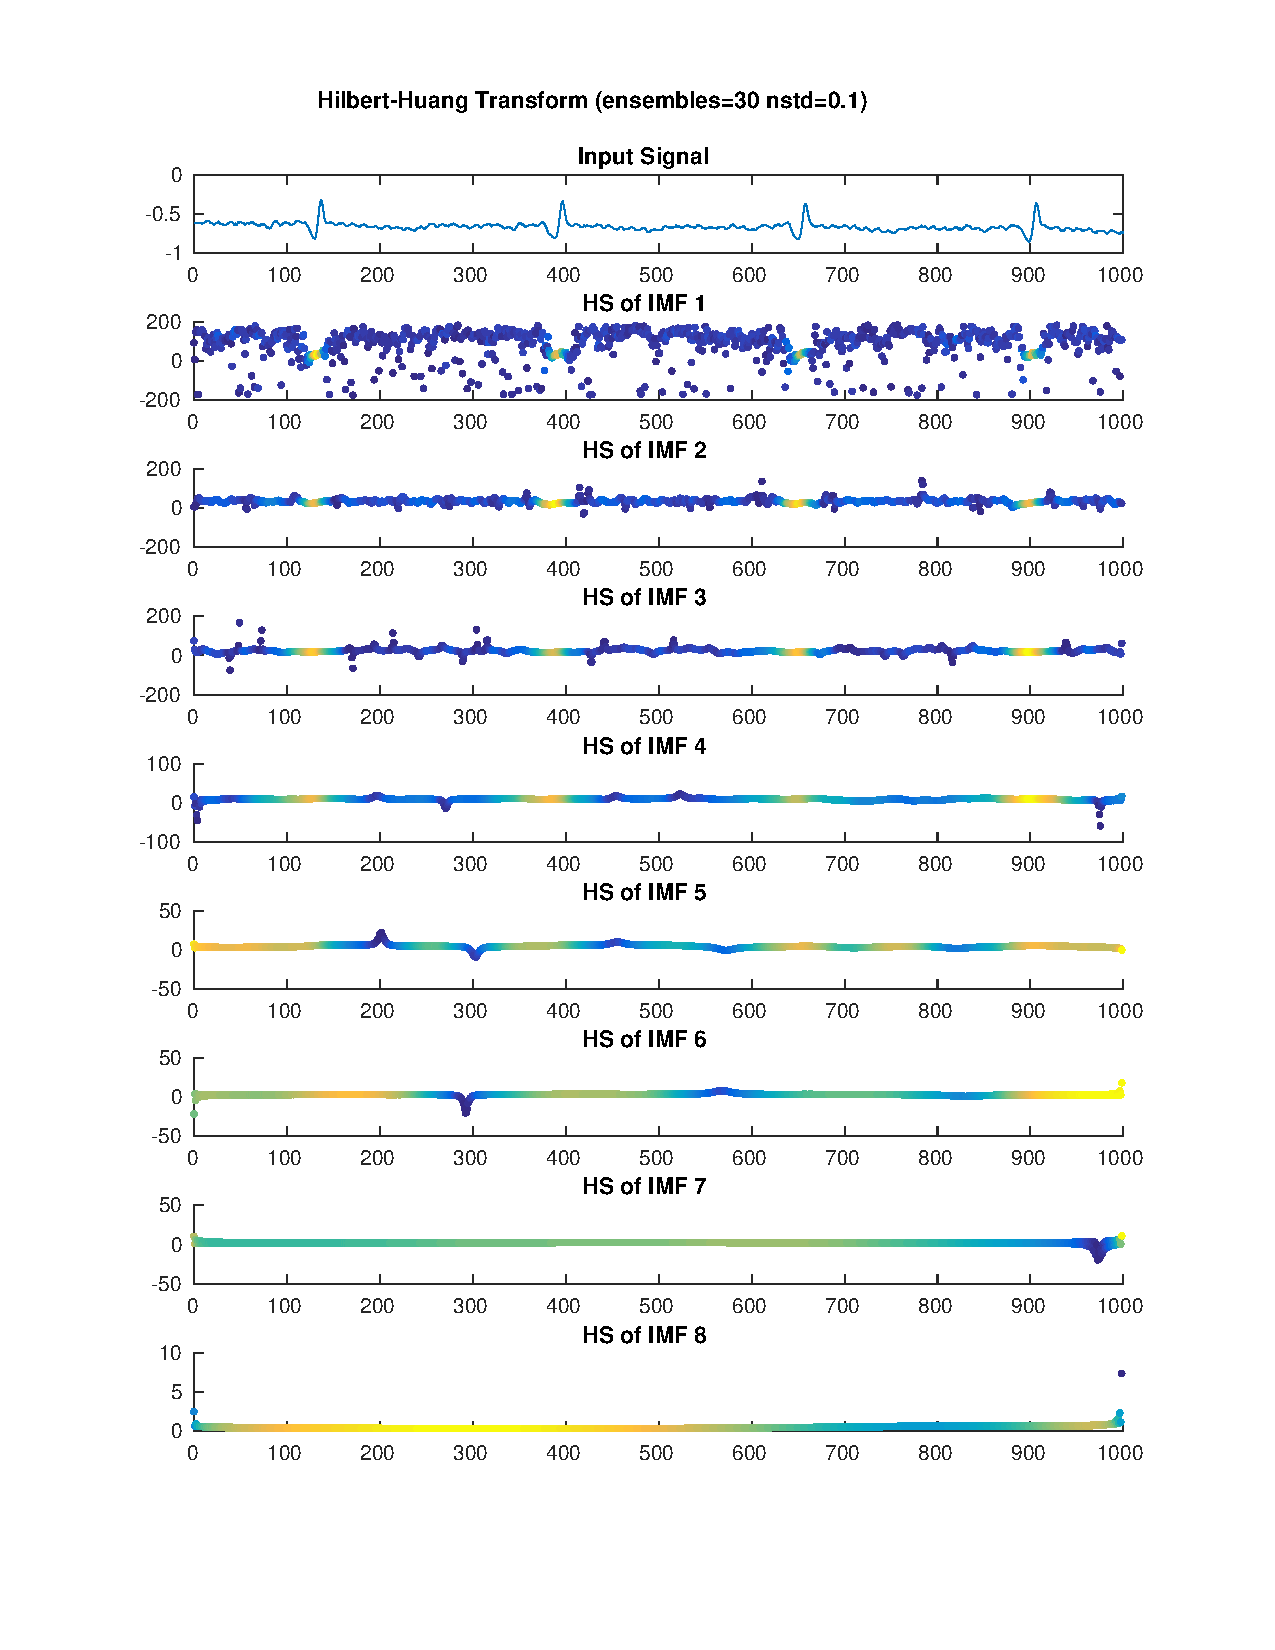
\includegraphics[width=\textwidth]{fig/112l2_hht_ensemble.pdf}
\end{minipage}
\vfill
\caption{EEMD και HHT με $n_{ens}=100$ και $\sigma_n = 0.1$.}
\label{fig:112l2_hht_ensemble}
\end{figure}


\subsubsection*{Σήμα 123}

% --- STFT, WDF, CWT ---
\begin{figure}[H]
\centering
\begin{minipage}{0.48\textwidth}
	\centering
	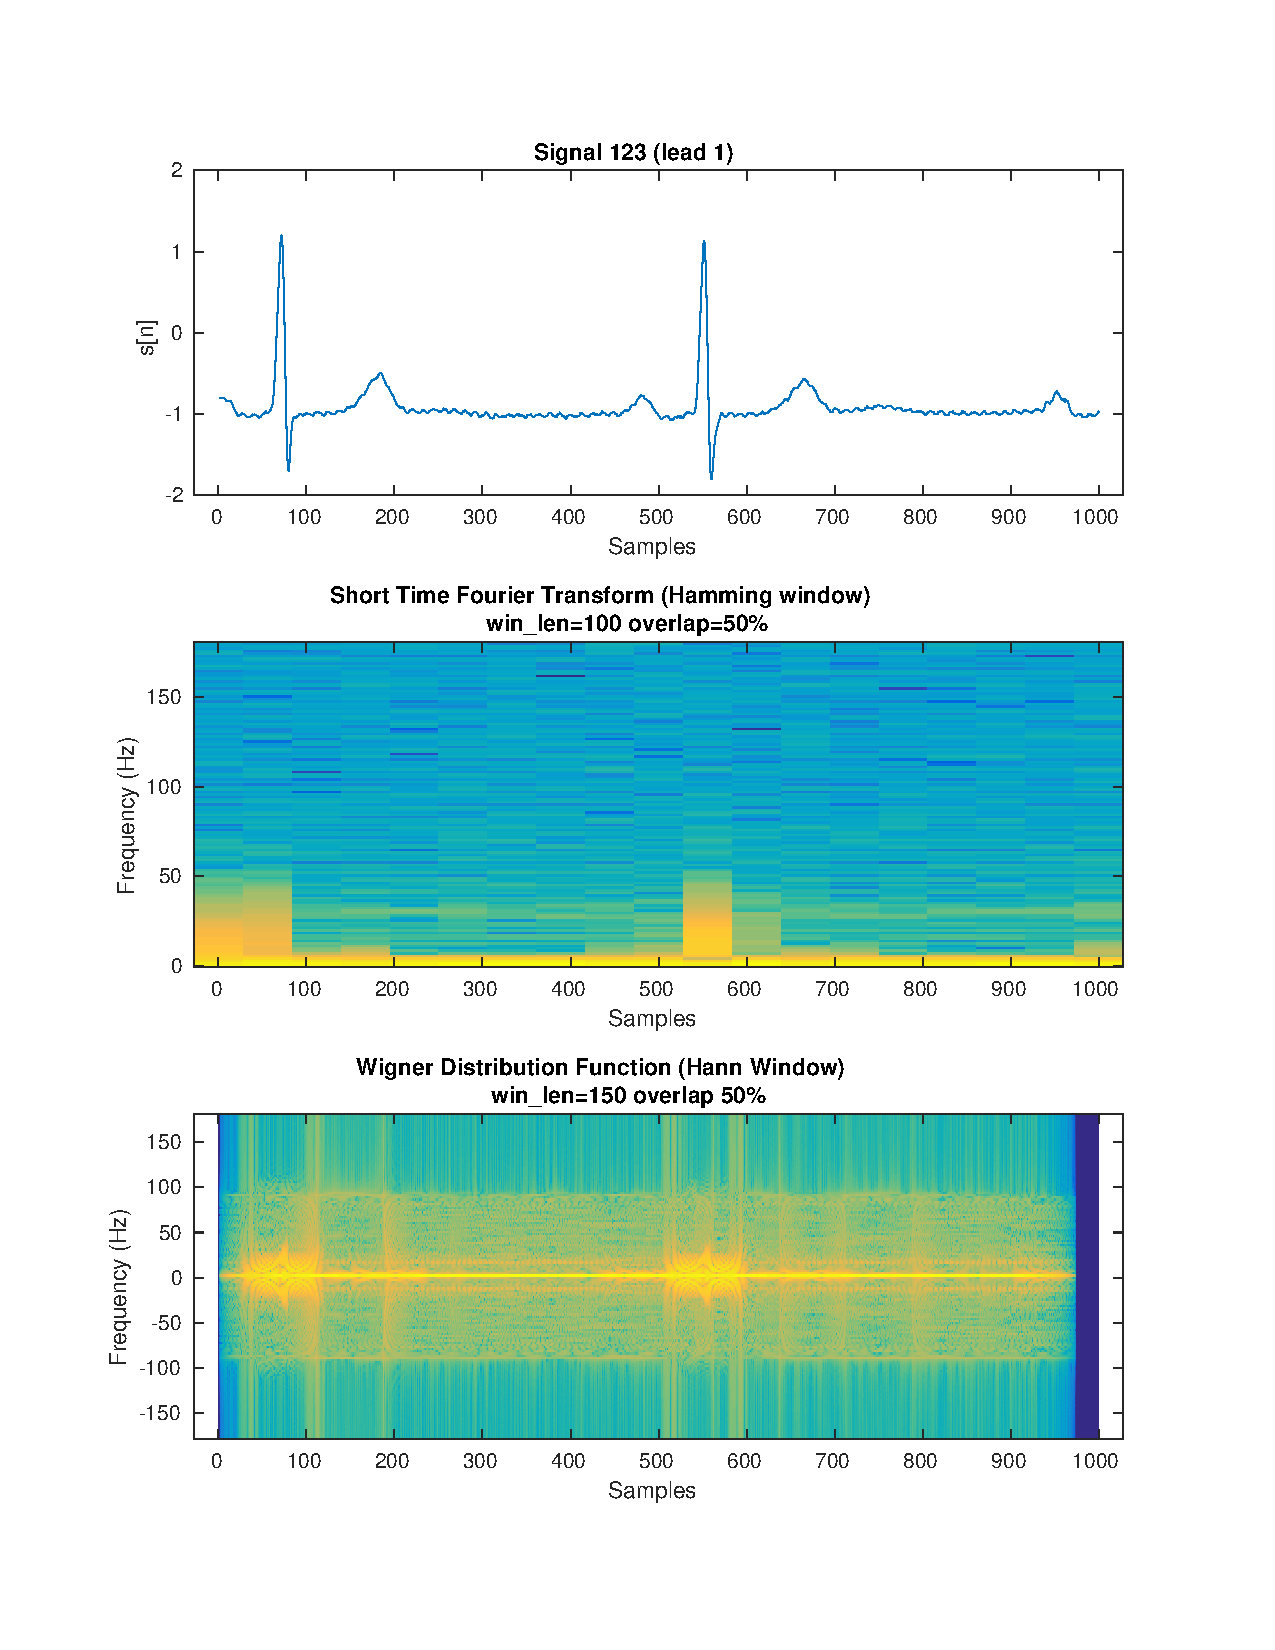
\includegraphics[width=\textwidth]{fig/123l1_stft_wdf.pdf}
\end{minipage}
\begin{minipage}{0.48\textwidth}
	\centering
	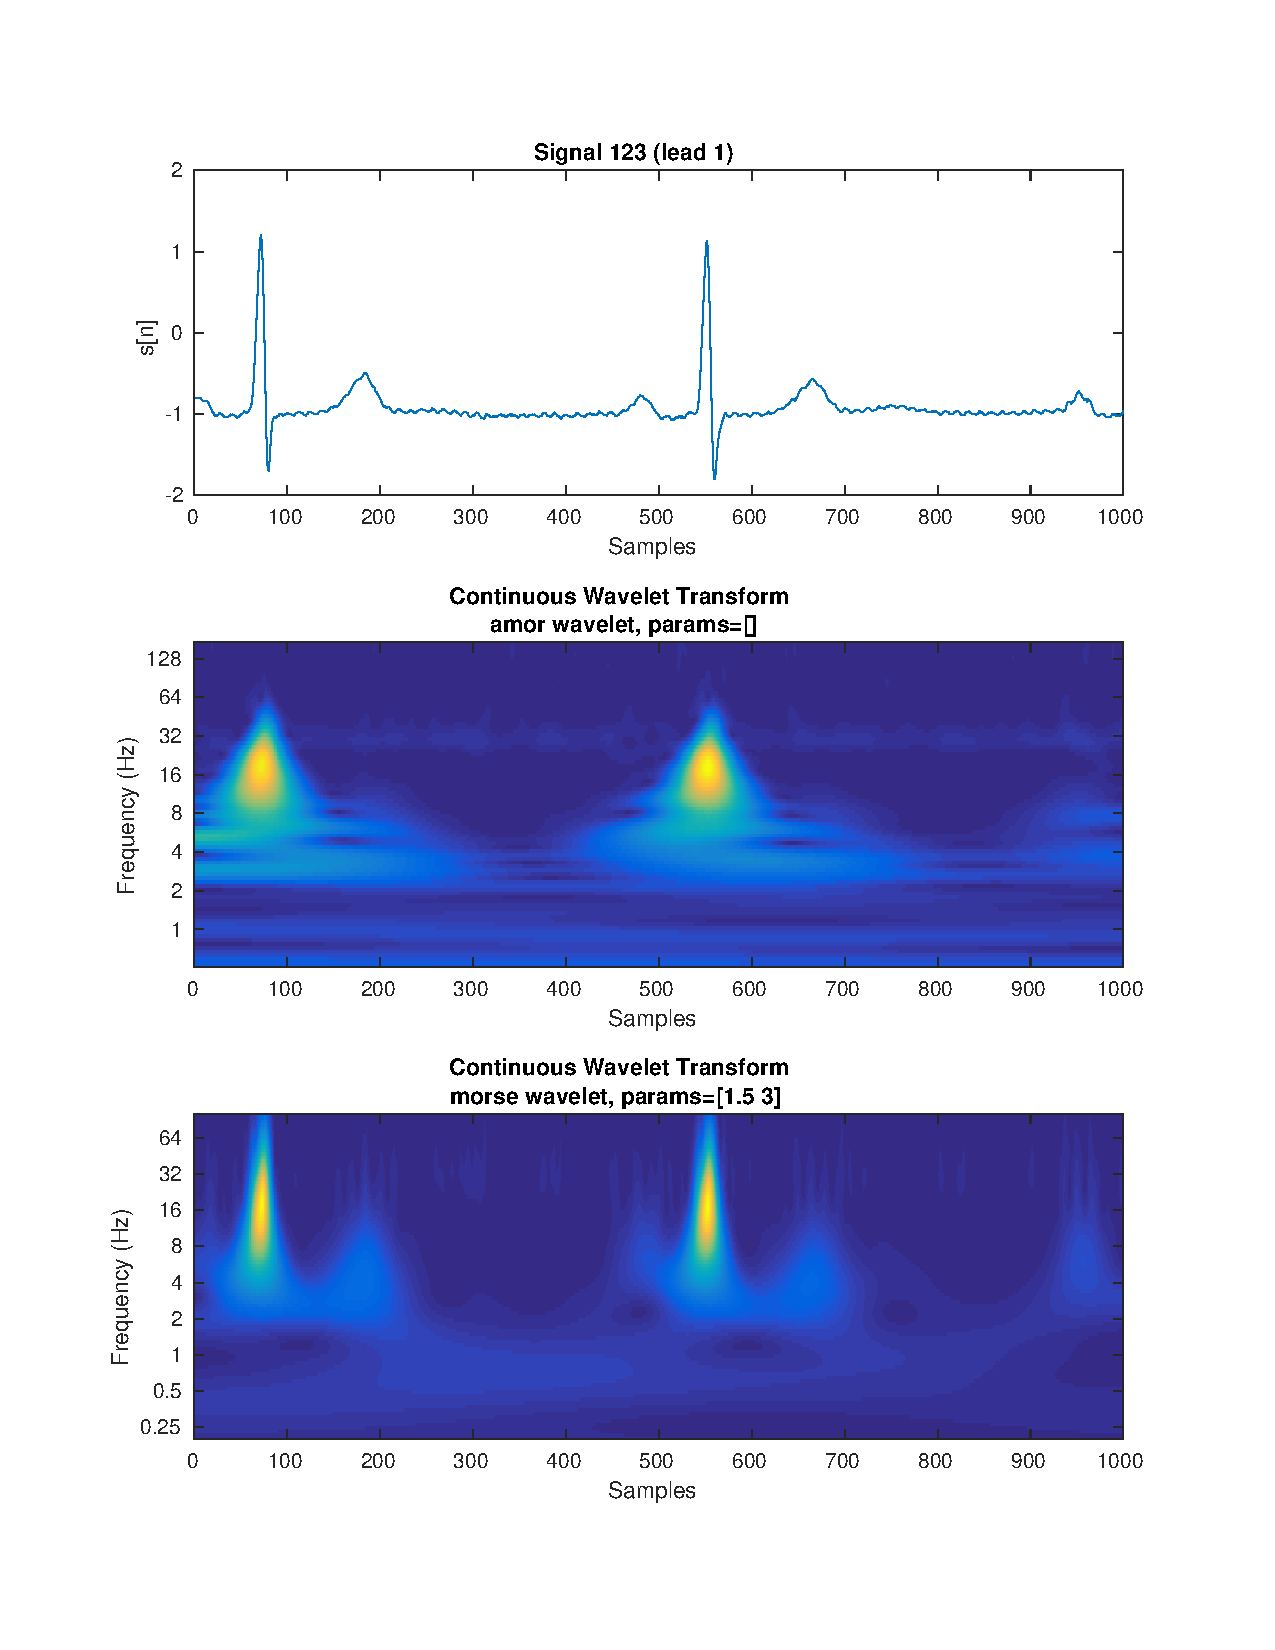
\includegraphics[width=\textwidth]{fig/123l1_cwt.pdf}
\end{minipage}
\vfill
\caption{STFT, WDF και συνεχής WT του σήματος 123. Η μεγαλύτερη απόσταση R-R μας επιτρέπει να επιλέξουμε πλατύτερο παράθυρο, κερδίζοντας ανάλυση στην συχνότητα.}
\label{fig:123l1_stft_wdf_wt}
\end{figure}


% --- DWT ---
\begin{figure}[H]
\centering
\begin{minipage}{0.48\textwidth}
	\centering
	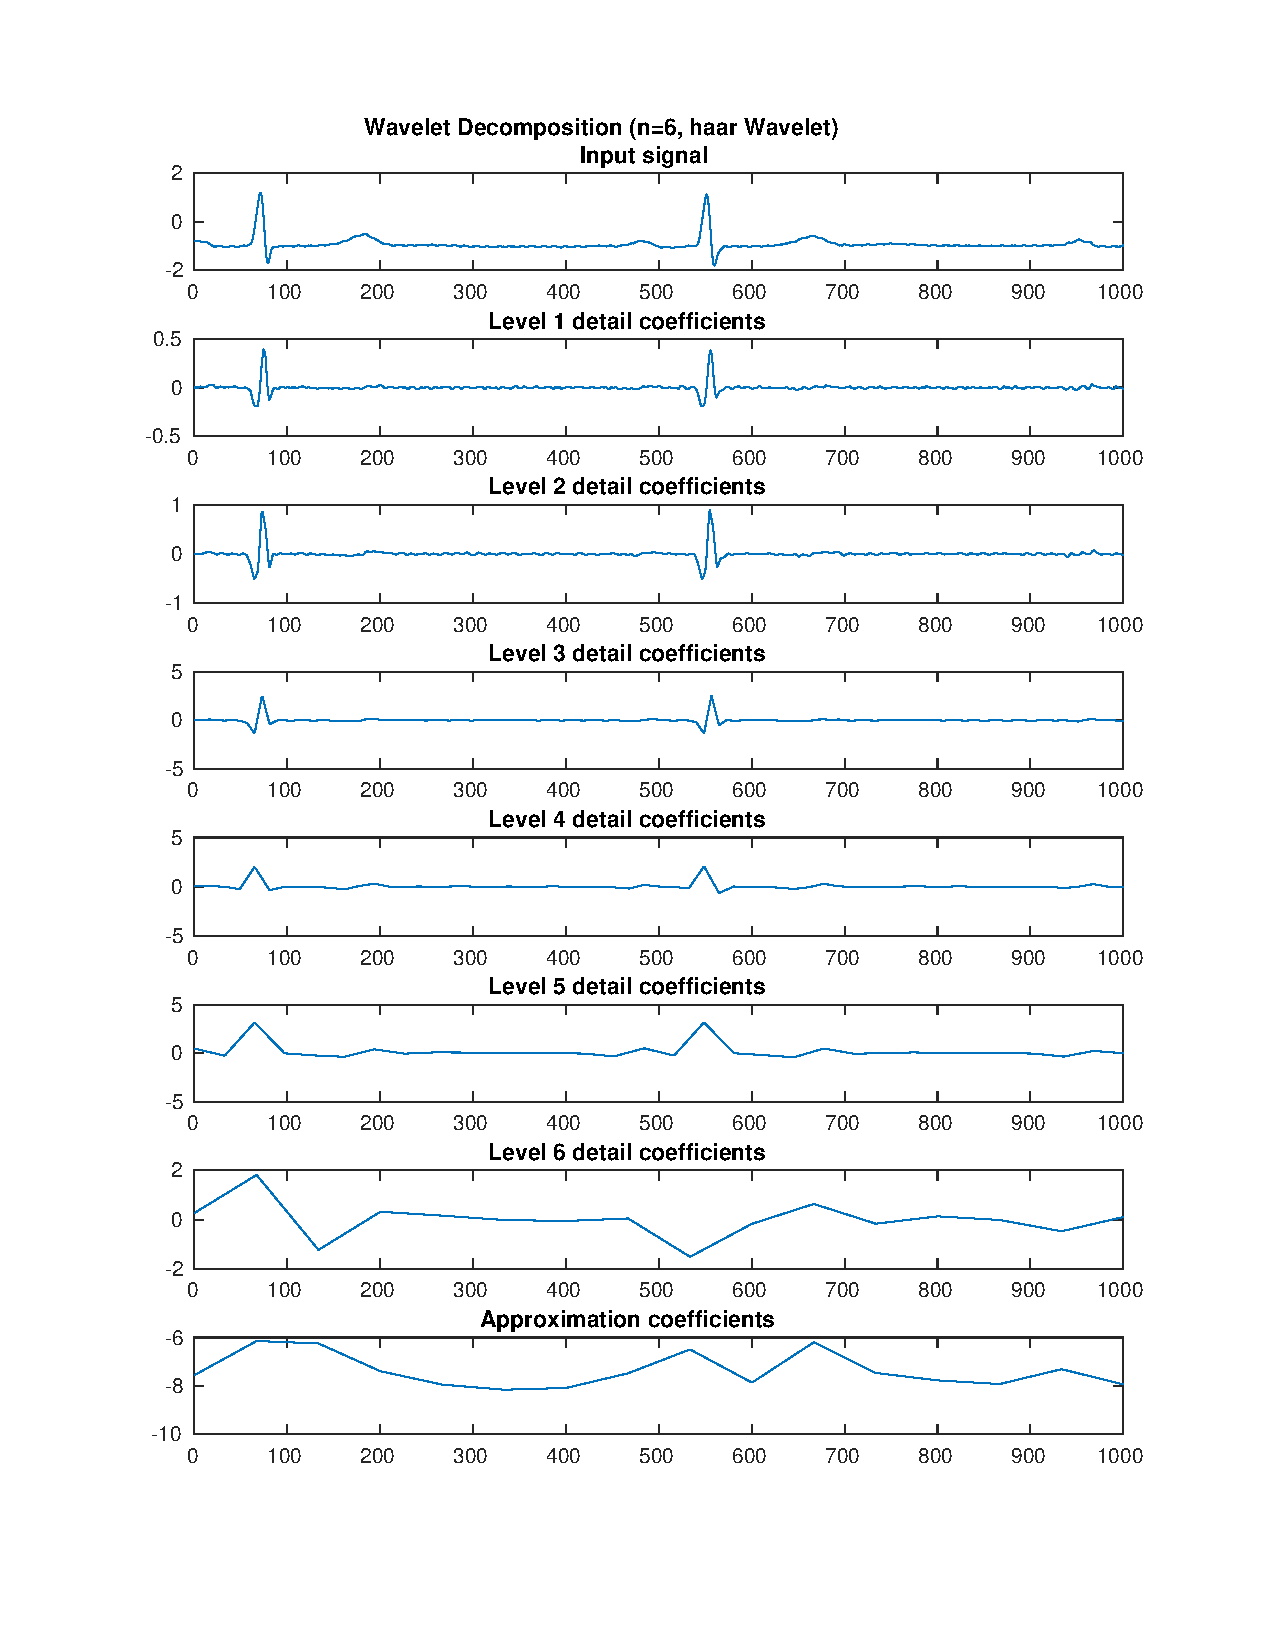
\includegraphics[width=\textwidth]{fig/123l1_dwt1.pdf}
\end{minipage}
\begin{minipage}{0.48\textwidth}
	\centering
	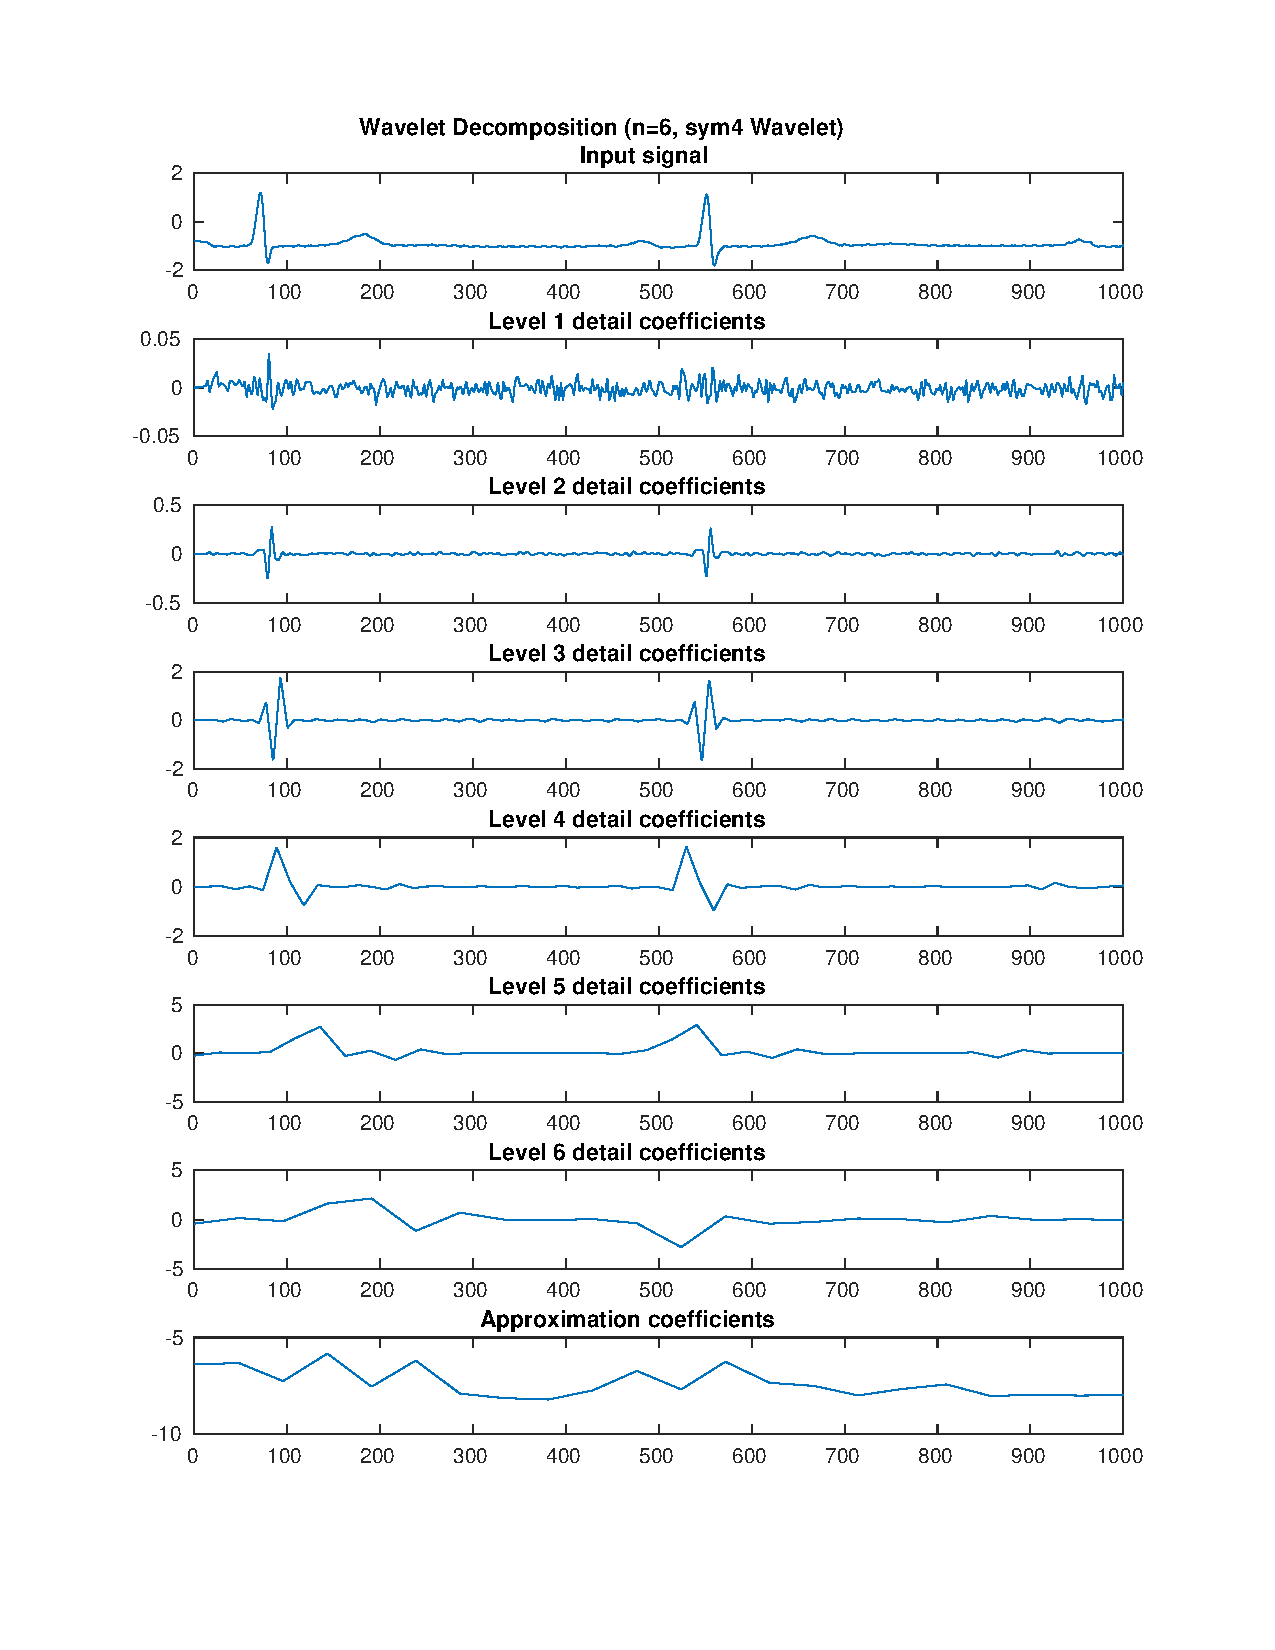
\includegraphics[width=\textwidth]{fig/123l1_dwt2.pdf}
\end{minipage}
\vfill
\caption{Διακριτός WT χρησιμοποιώντας db4 και bior1.3. Το $d_1$ με db4 περιέχει κυρίως θόρυβο. Τα $d_{2-5}$ αναπαριστούν ικανοποιητικά τα QRS complexes.}
\label{fig:123l1_dwt}
\end{figure}


% --- EMD/HHT ---
\begin{figure}[H]
\centering
\begin{minipage}{0.48\textwidth}
	\centering
	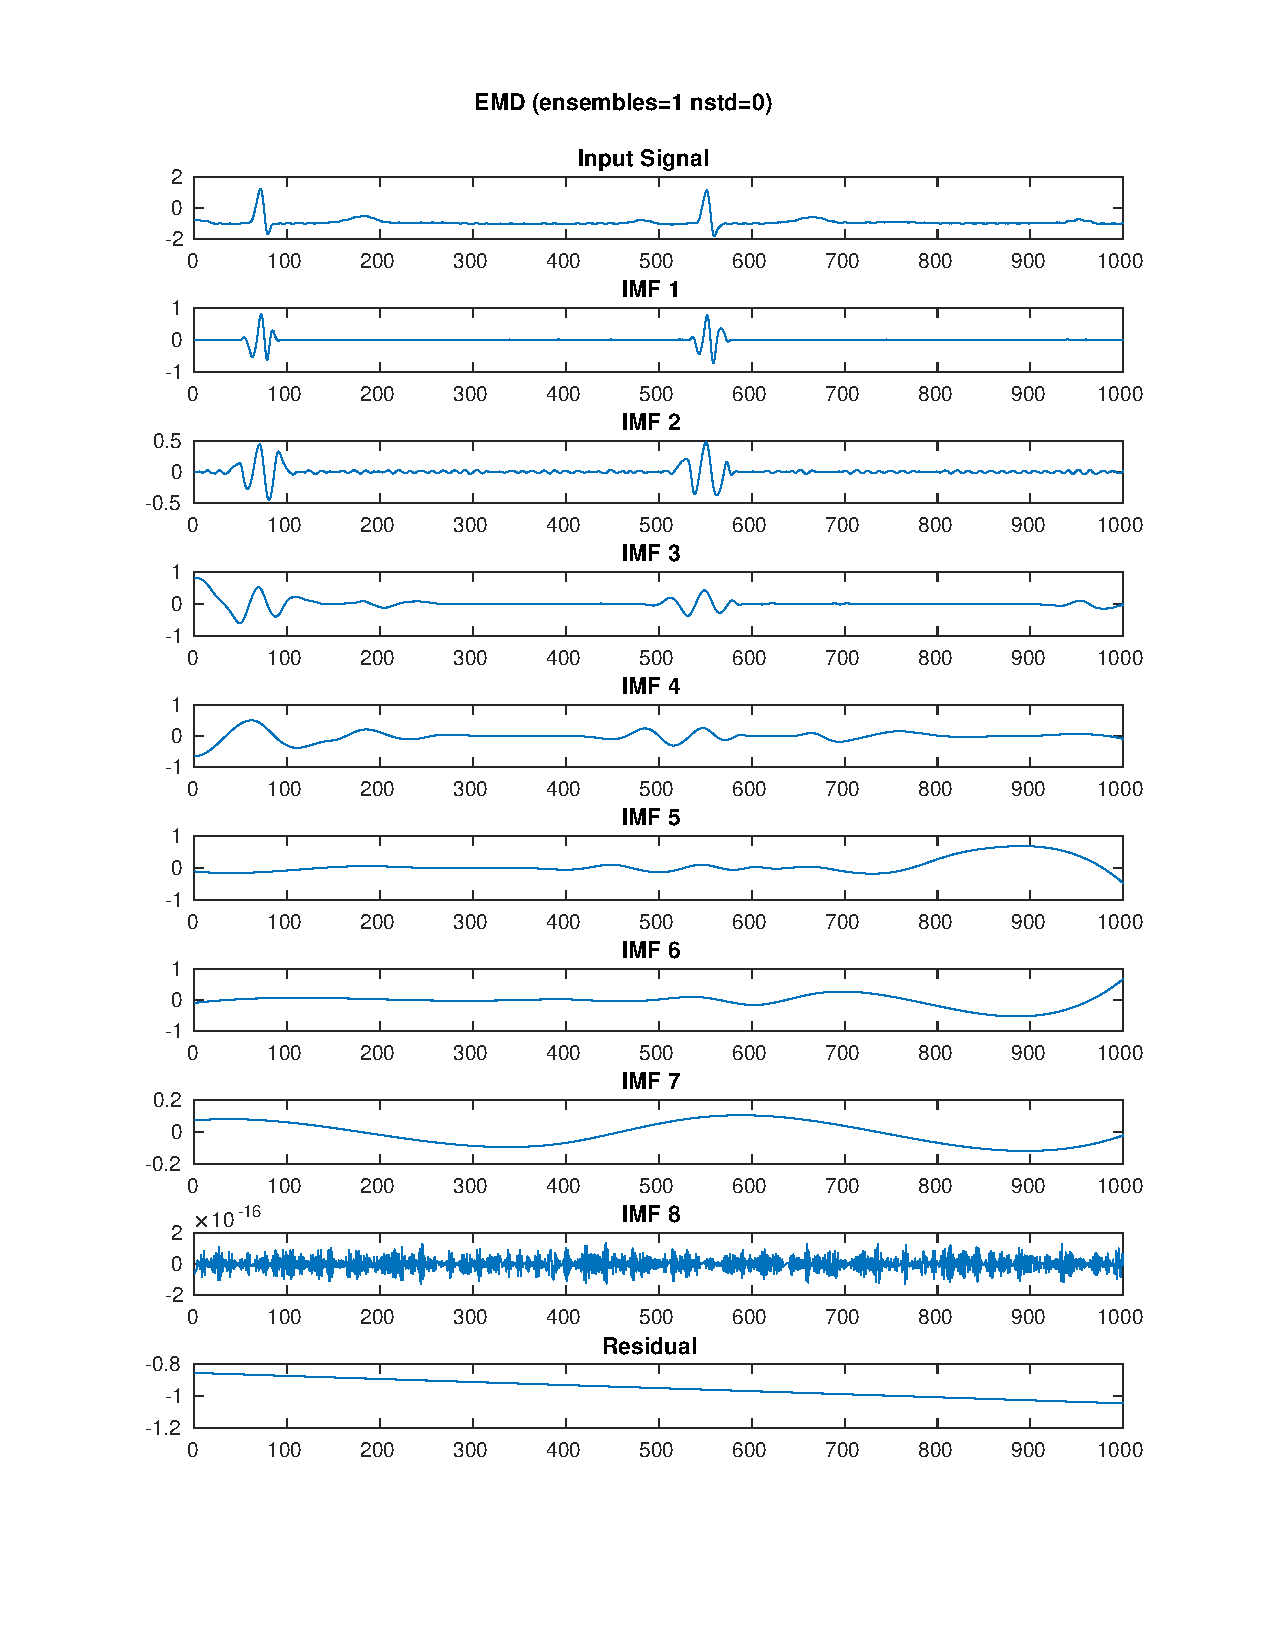
\includegraphics[width=\textwidth]{fig/123l1_emd.pdf}
\end{minipage}
\begin{minipage}{0.48\textwidth}
	\centering
	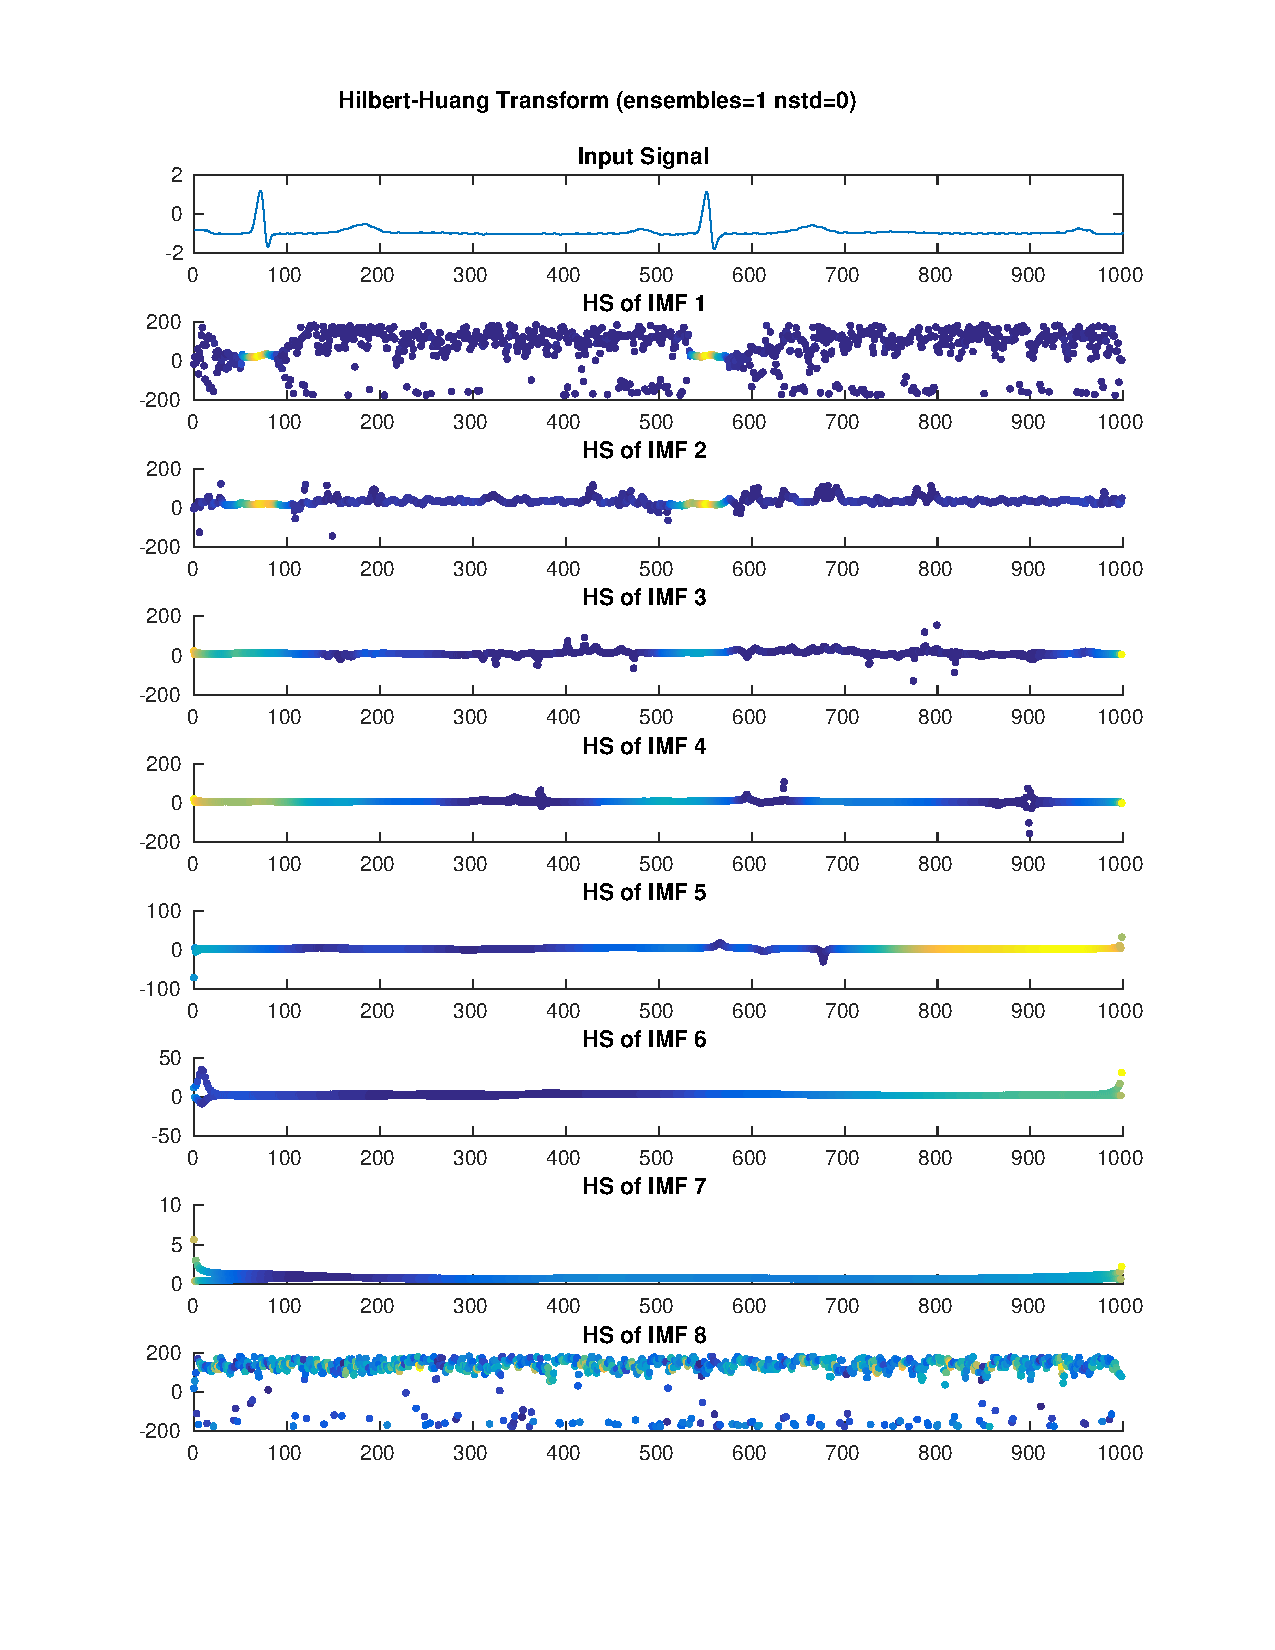
\includegraphics[width=\textwidth]{fig/123l1_hht.pdf}
\end{minipage}
\vfill
\caption{EMD και HHT του σήματος 123. Δεν εμφανίζεται έντονο mode mixing.}
\label{fig:123l1_hht}
\end{figure}


% --- EEMD/HHT ---
\begin{figure}[H]
\centering
\begin{minipage}{0.48\textwidth}
	\centering
	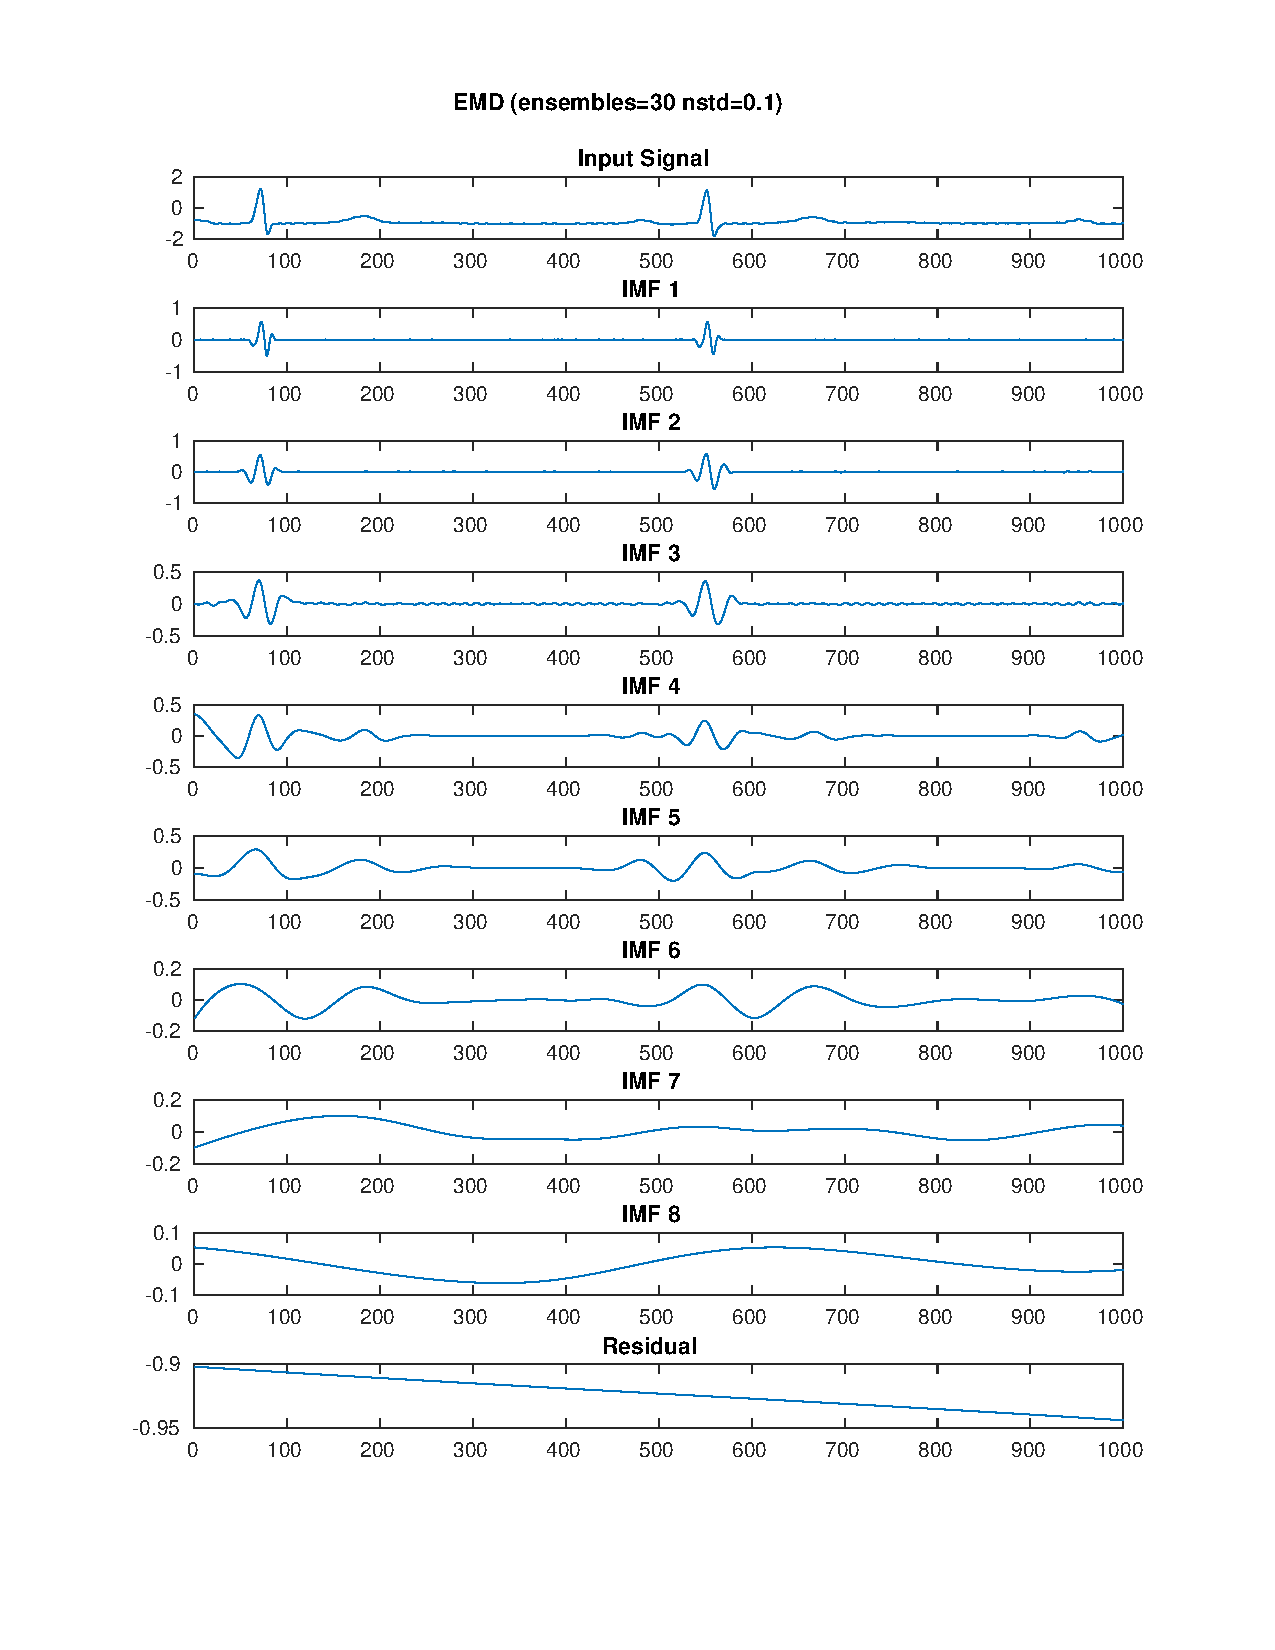
\includegraphics[width=\textwidth]{fig/123l1_emd_ensemble.pdf}
\end{minipage}
\begin{minipage}{0.48\textwidth}
	\centering
	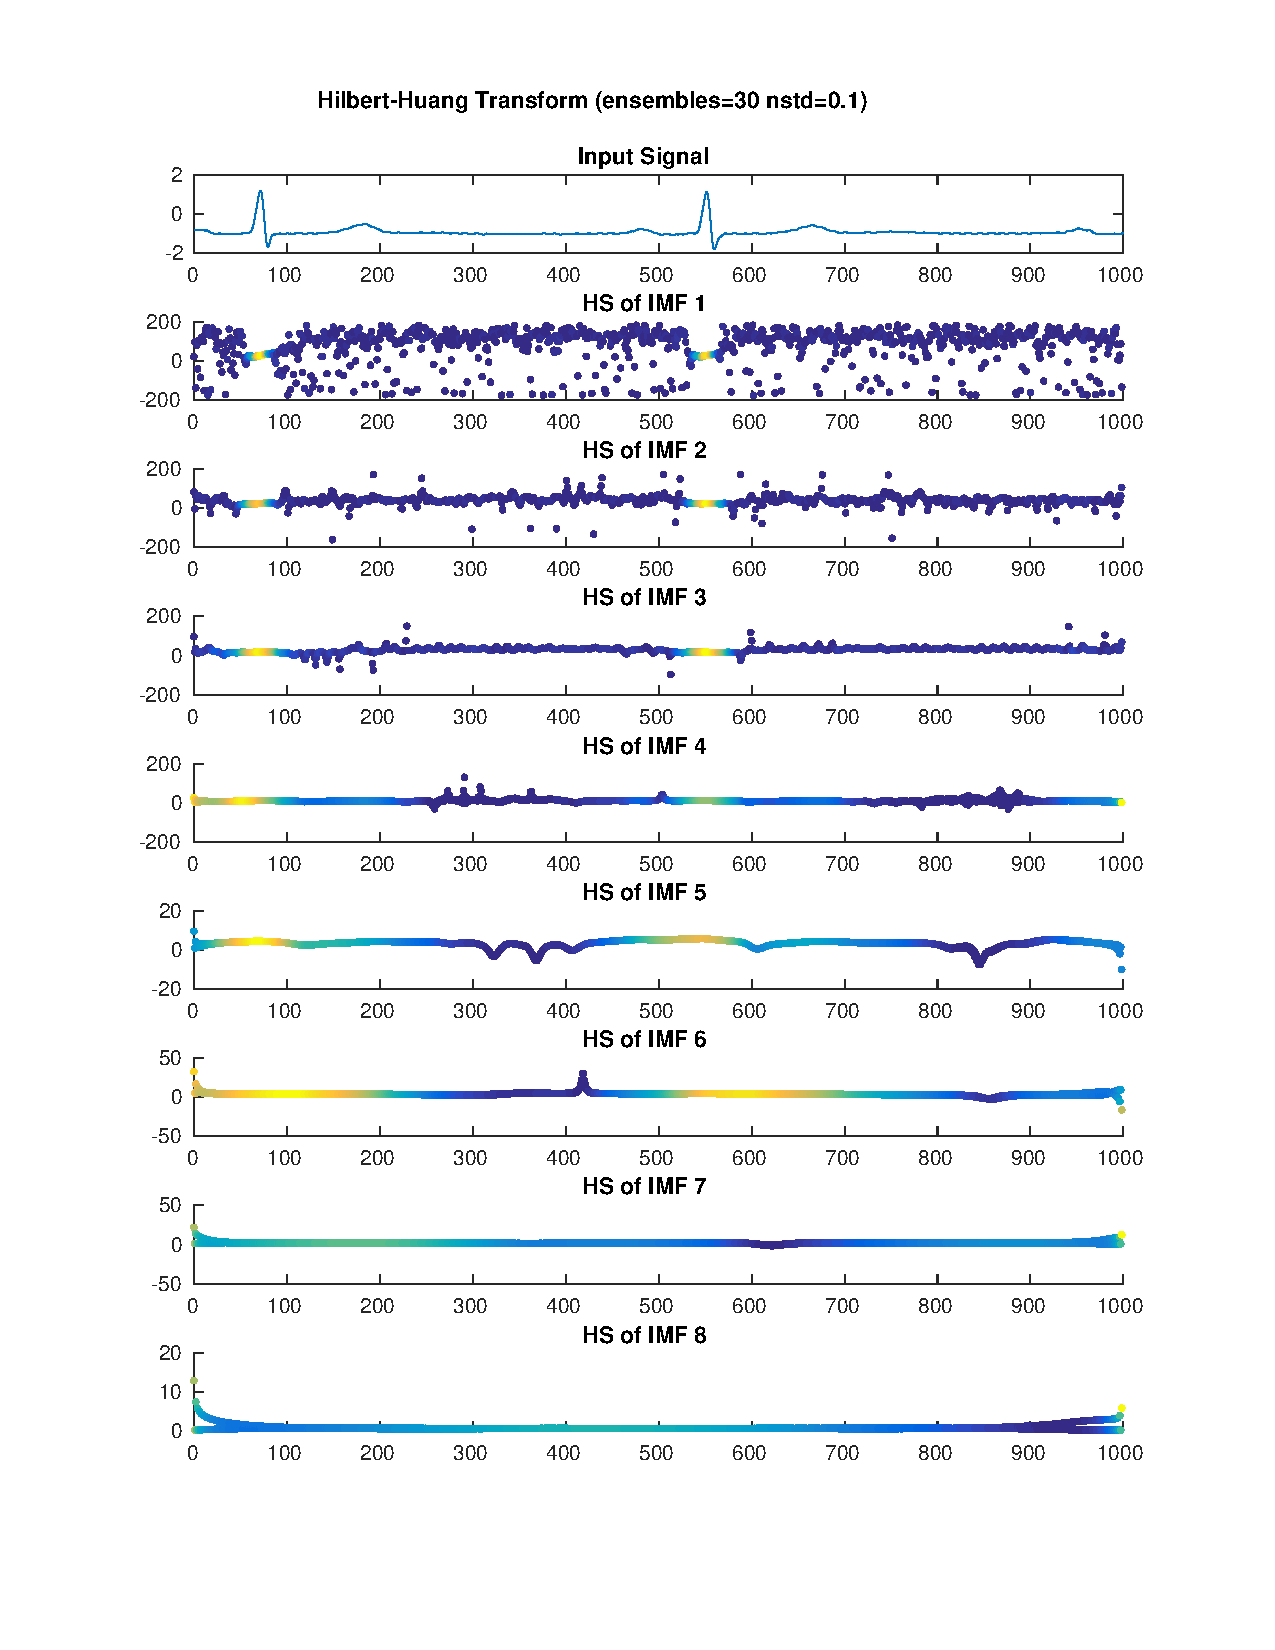
\includegraphics[width=\textwidth]{fig/123l1_hht_ensemble.pdf}
\end{minipage}
\vfill
\caption{EEMD και HHT με $n_{ens}=100$ και $\sigma_n = 0.1$. Η εφαρμογή του EEMD είναι περιττή καθώς δεν υπήρχε ισχυρό mode mixing.}
\label{fig:123l1_hht_ensemble}
\end{figure}

\subsubsection*{Σήμα 118}

% --- STFT, WDF, CWT ---
\begin{figure}[H]
\centering
\begin{minipage}{0.48\textwidth}
	\centering
	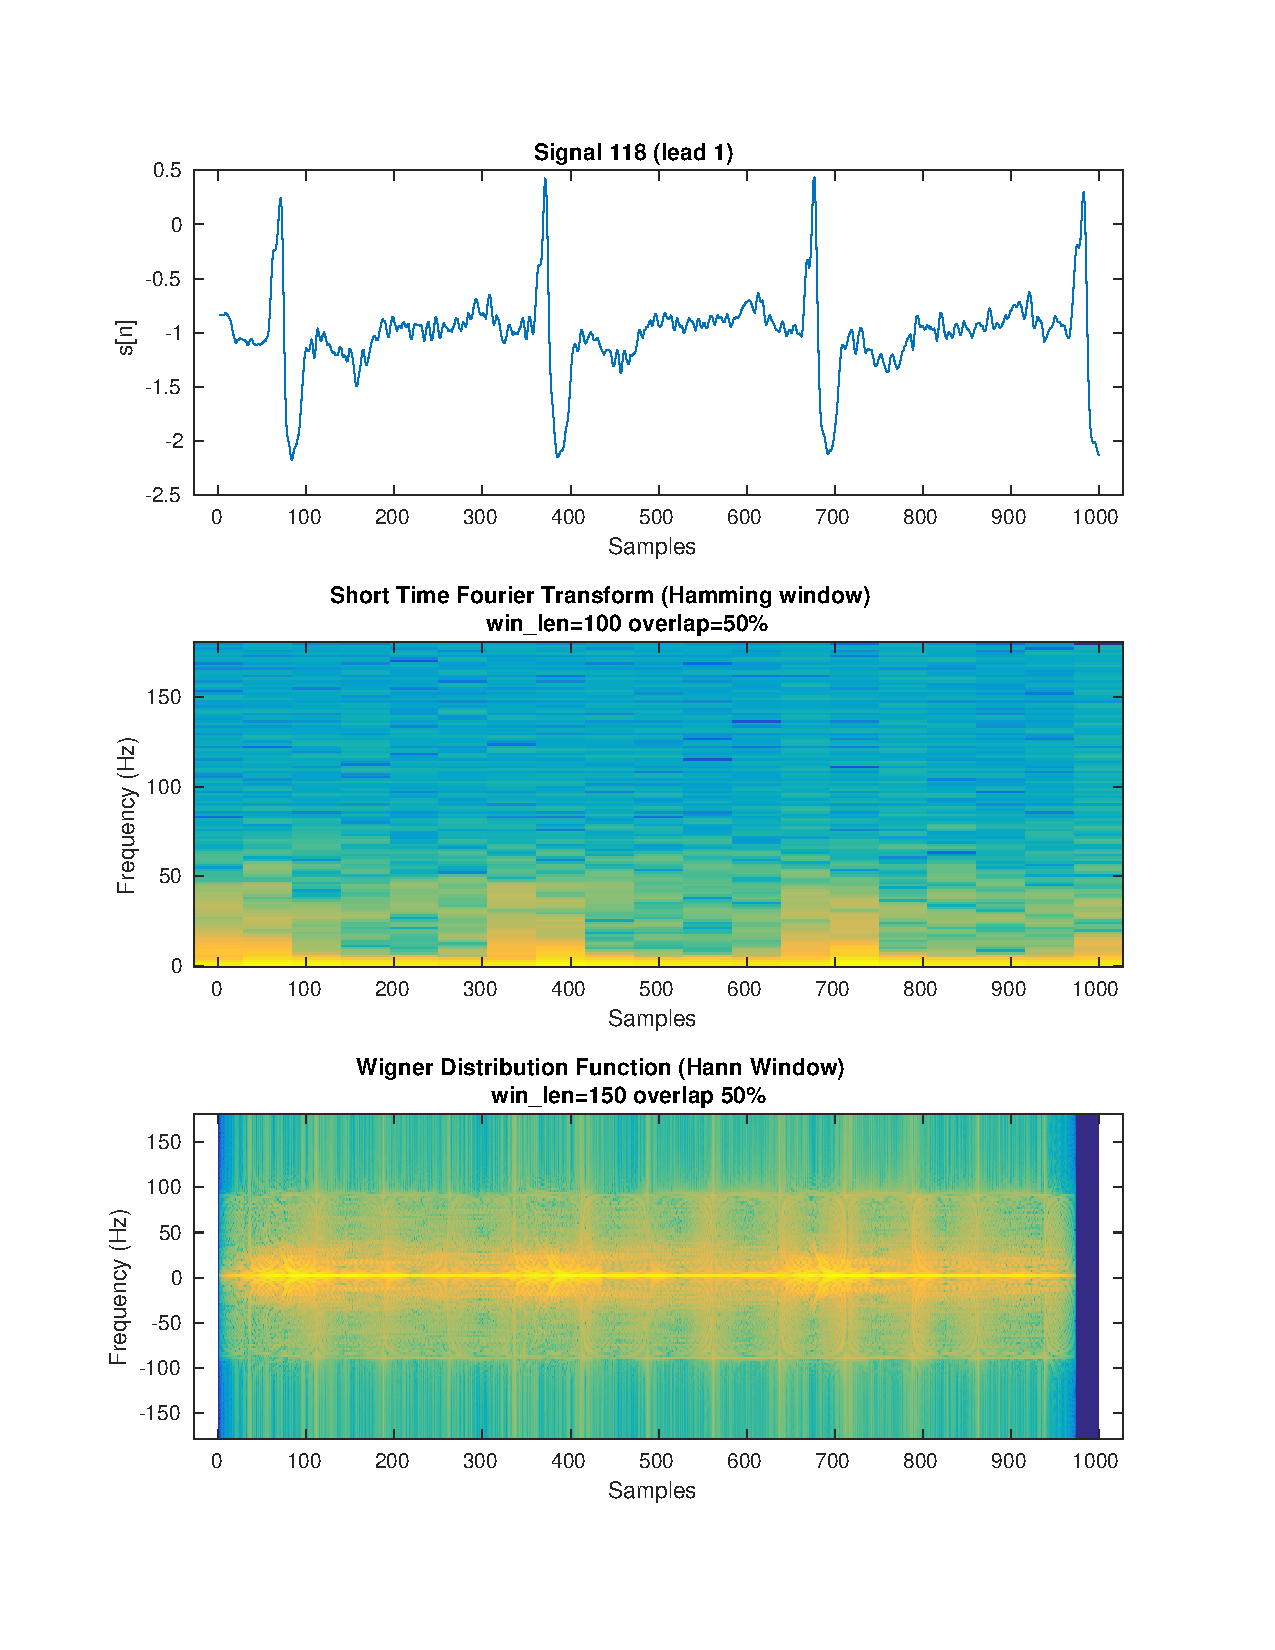
\includegraphics[width=\textwidth]{fig/118l1_stft_wdf.pdf}
\end{minipage}
\begin{minipage}{0.48\textwidth}
	\centering
	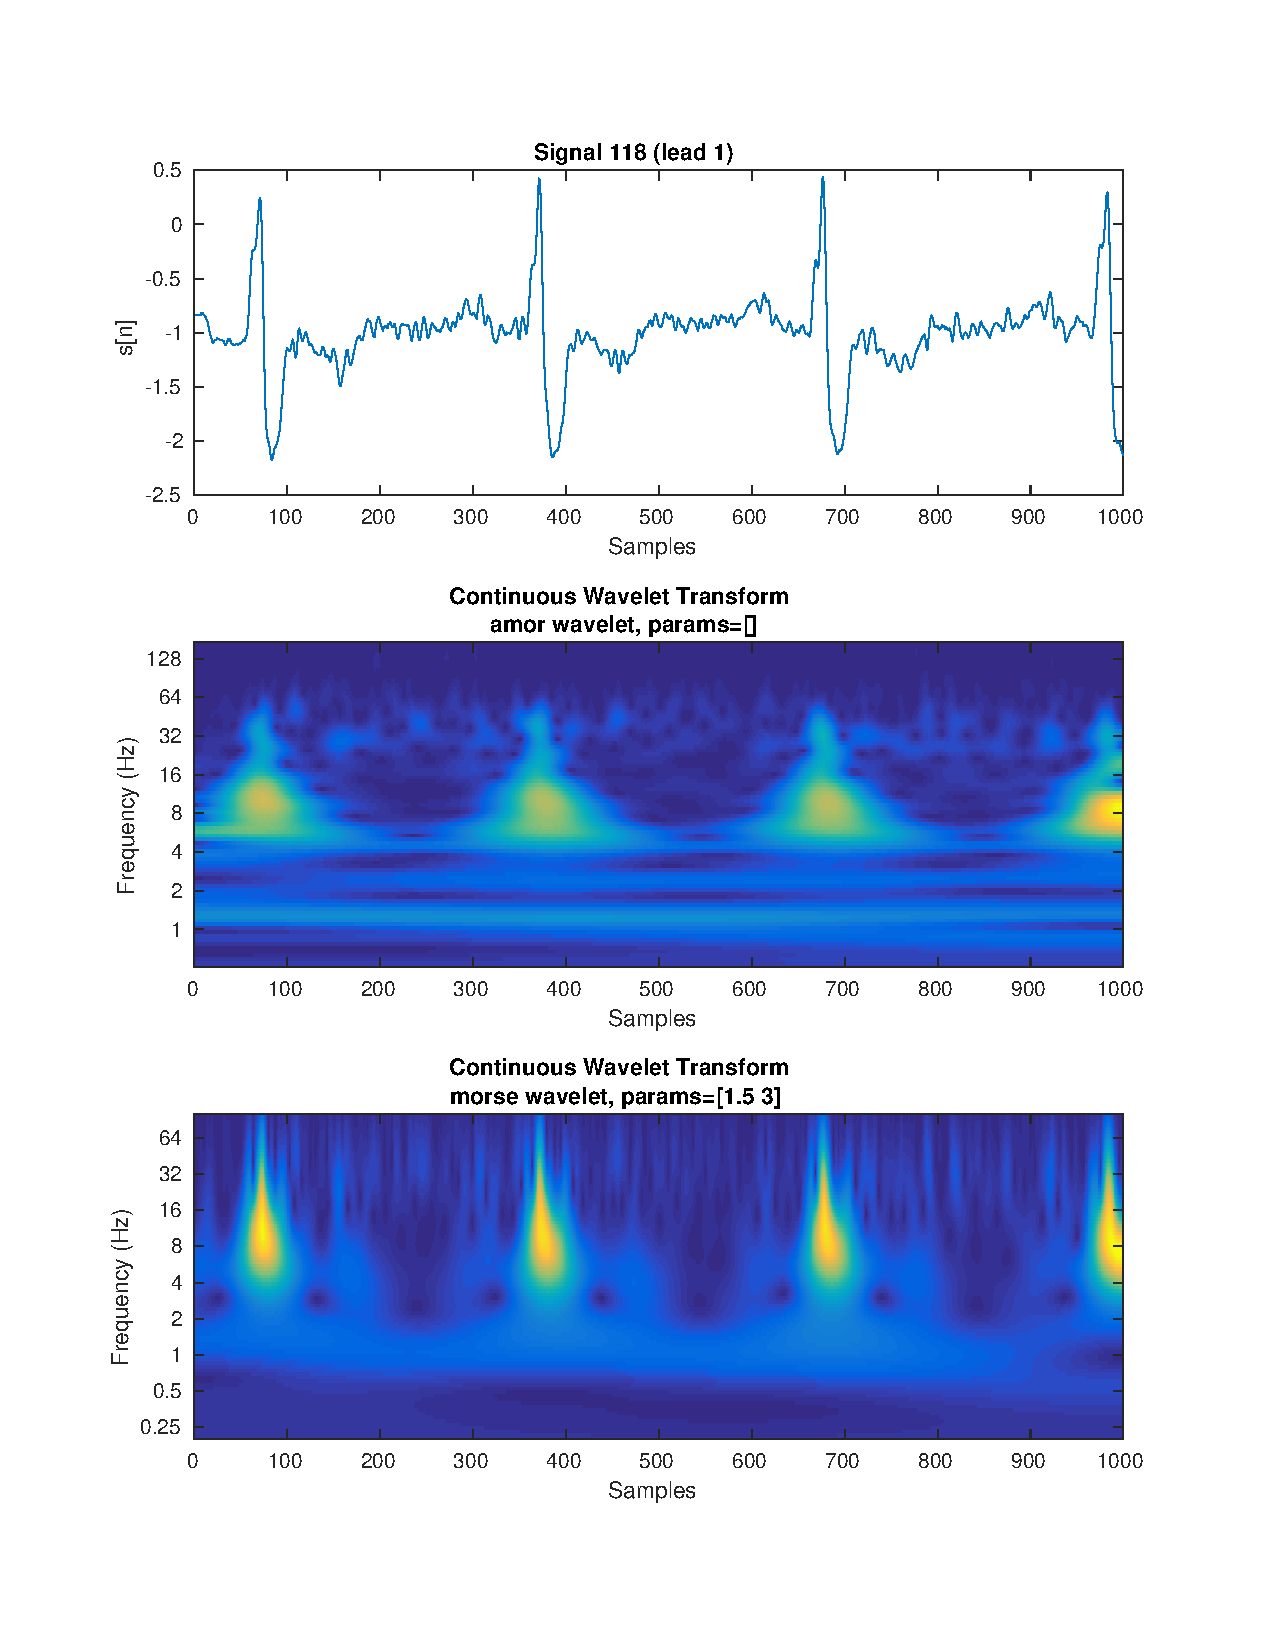
\includegraphics[width=\textwidth]{fig/118l1_cwt.pdf}
\end{minipage}
\vfill
\caption{STFT, WDF και συνεχής WT του σήματος 118. Η μεγαλύτερη διάρκεια του QRS complex, λόγω του RBBB, παρατηρείται στον WT με Morlet Wavelet (amor).}
\label{fig:118l1_stft_wdf_wt}
\end{figure}


% --- DWT ---
\begin{figure}[H]
\centering
\begin{minipage}{0.48\textwidth}
	\centering
	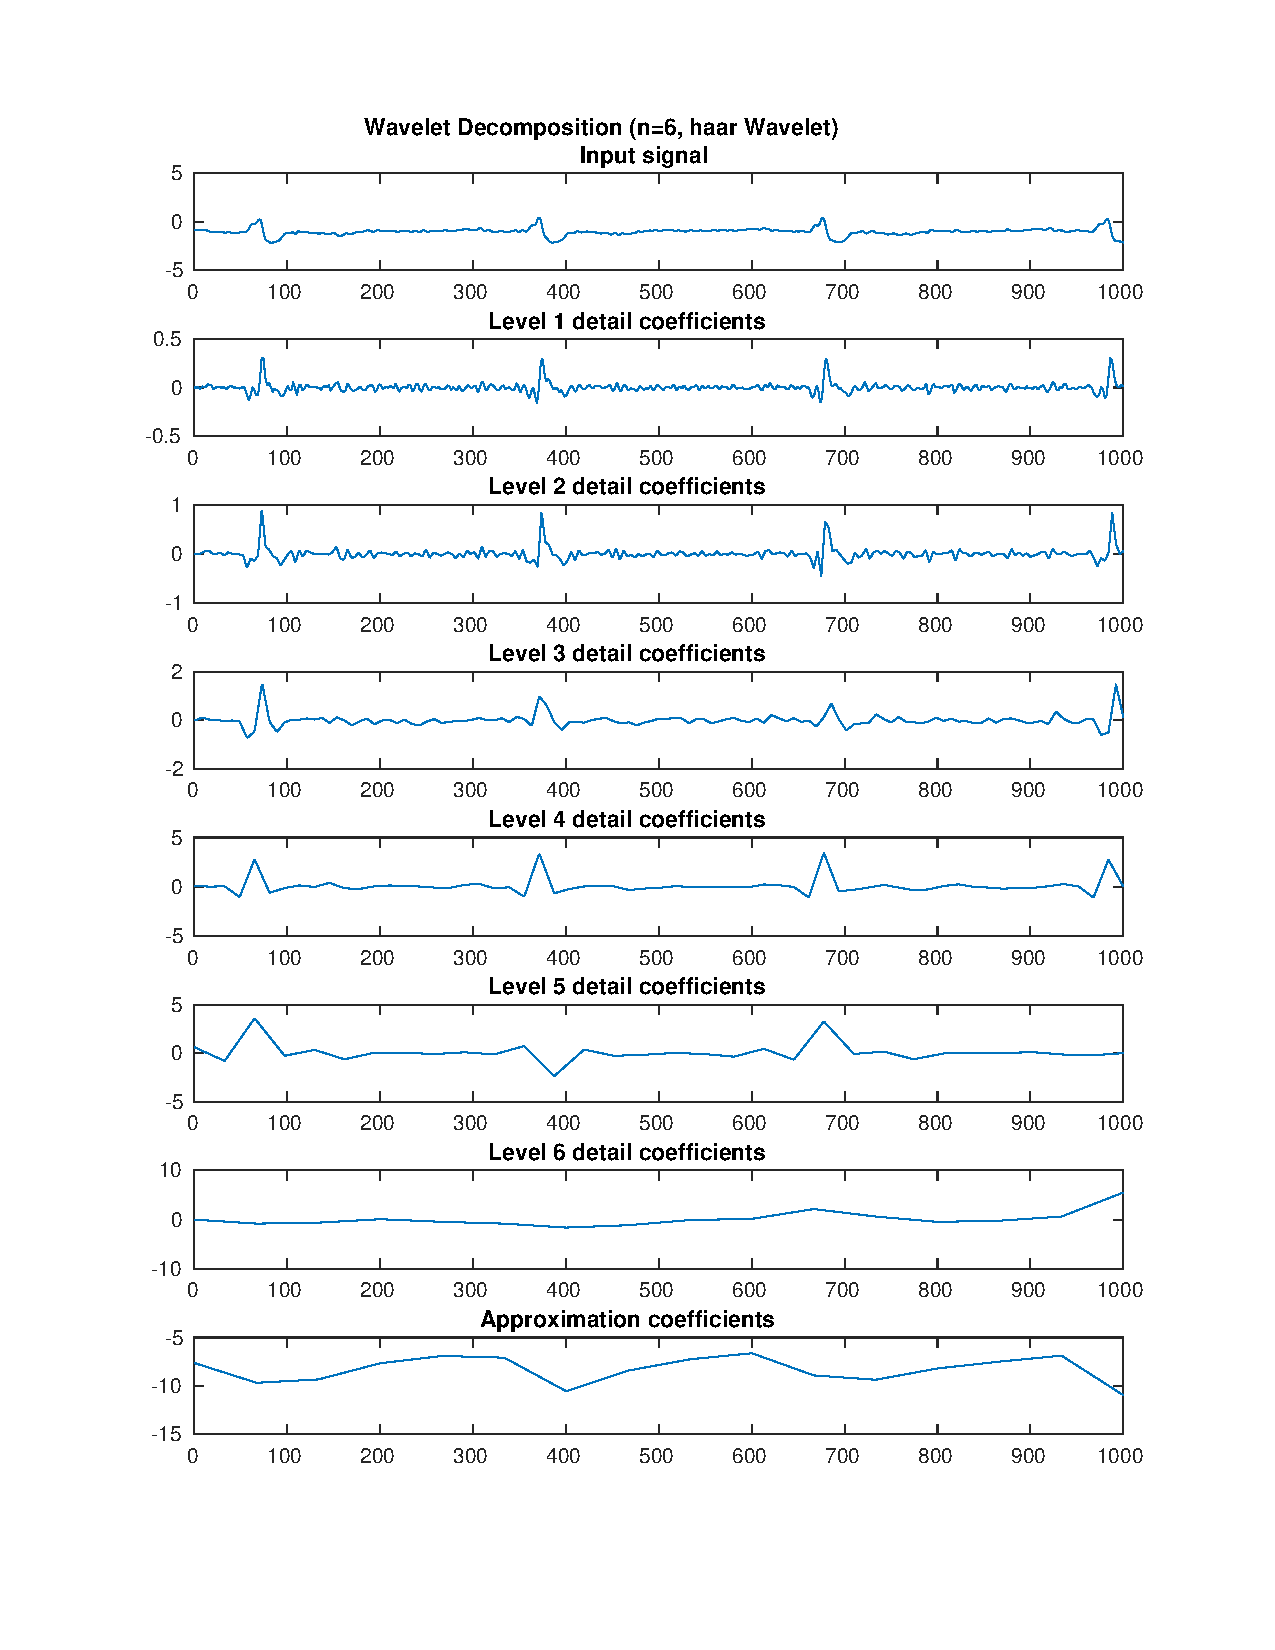
\includegraphics[width=\textwidth]{fig/118l1_dwt1.pdf}
\end{minipage}
\begin{minipage}{0.48\textwidth}
	\centering
	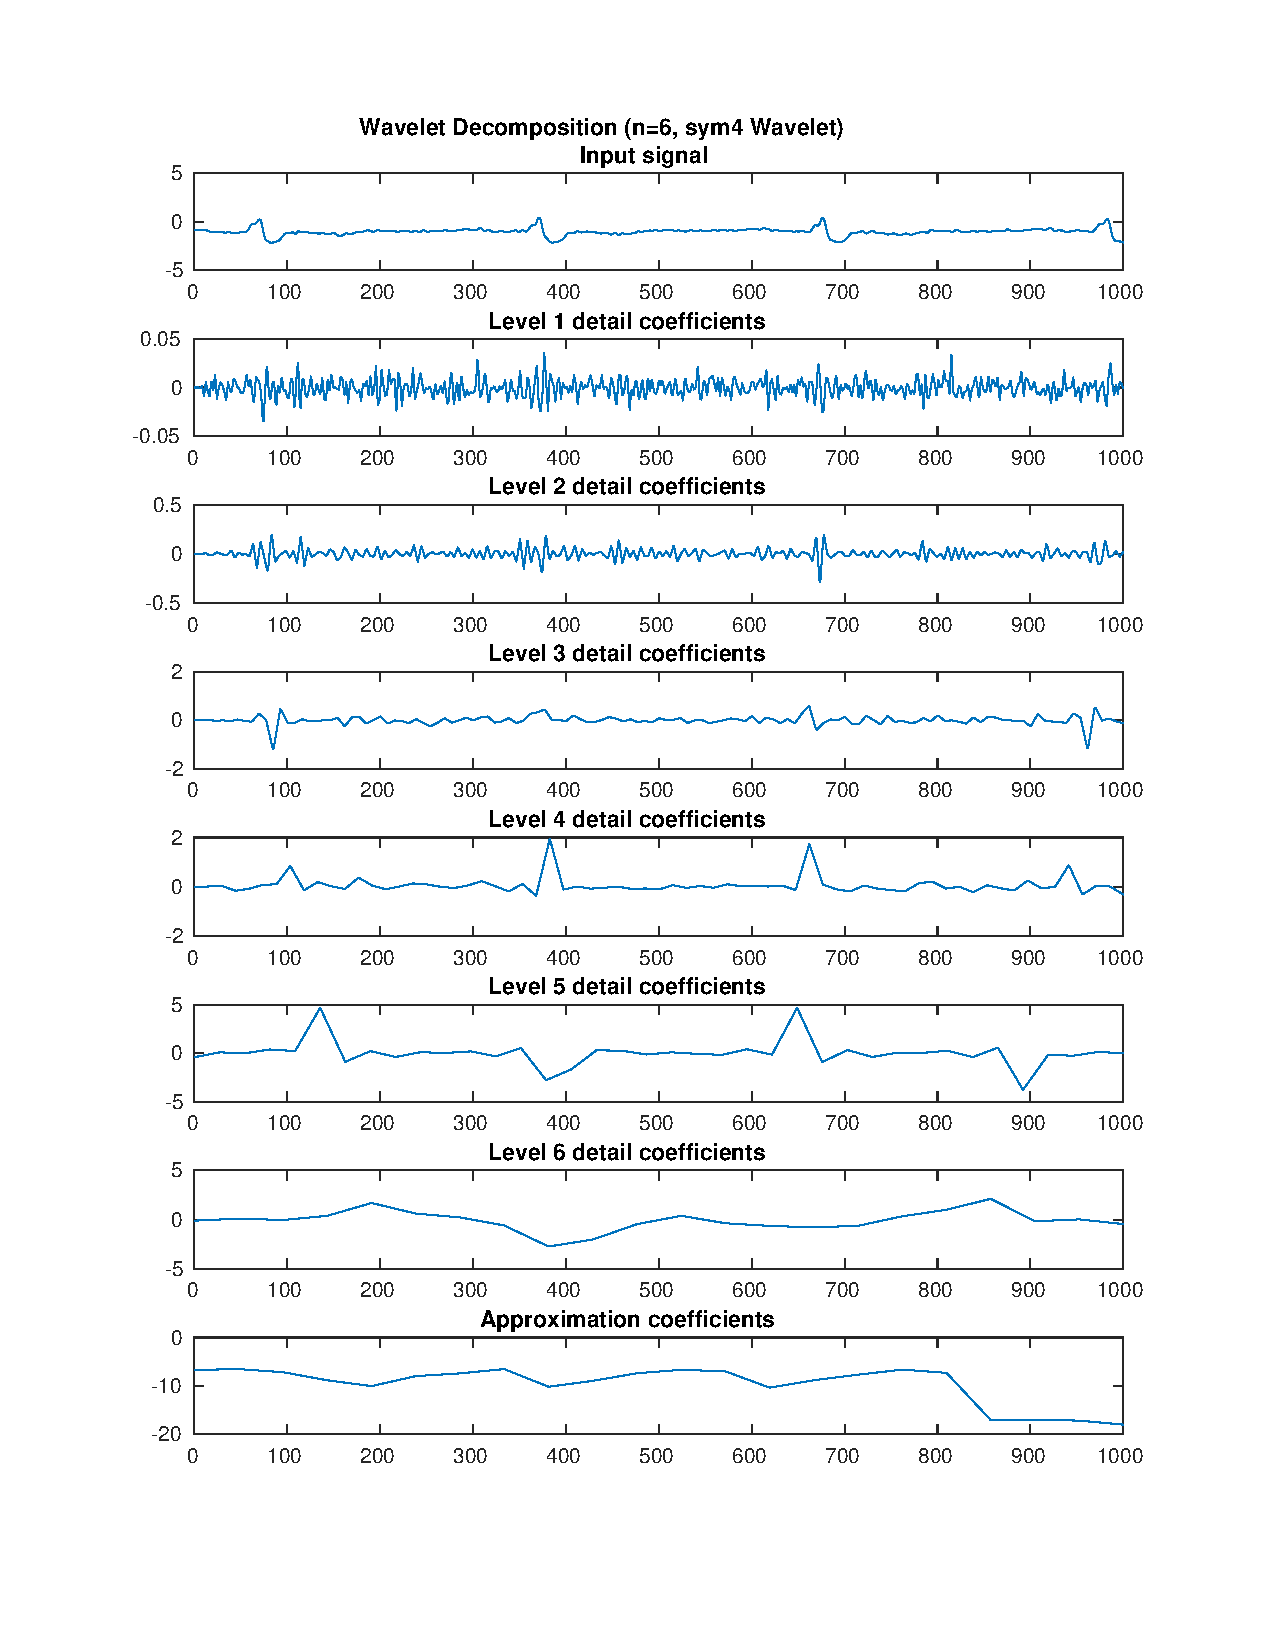
\includegraphics[width=\textwidth]{fig/118l1_dwt2.pdf}
\end{minipage}
\vfill
\caption{Διακριτός WT χρησιμοποιώντας db4 και bior1.3. Οι συντελεστές $d_6$ εμφανίζουν πιο αργές ταλαντώσεις σε σύγκριση με τα προηγούμενα σήματα, γεγονός που οφείλεται στο RBBB.}
\label{fig:118l1_dwt}
\end{figure}


% --- EMD/HHT ---
\begin{figure}[H]
\centering
\begin{minipage}{0.48\textwidth}
	\centering
	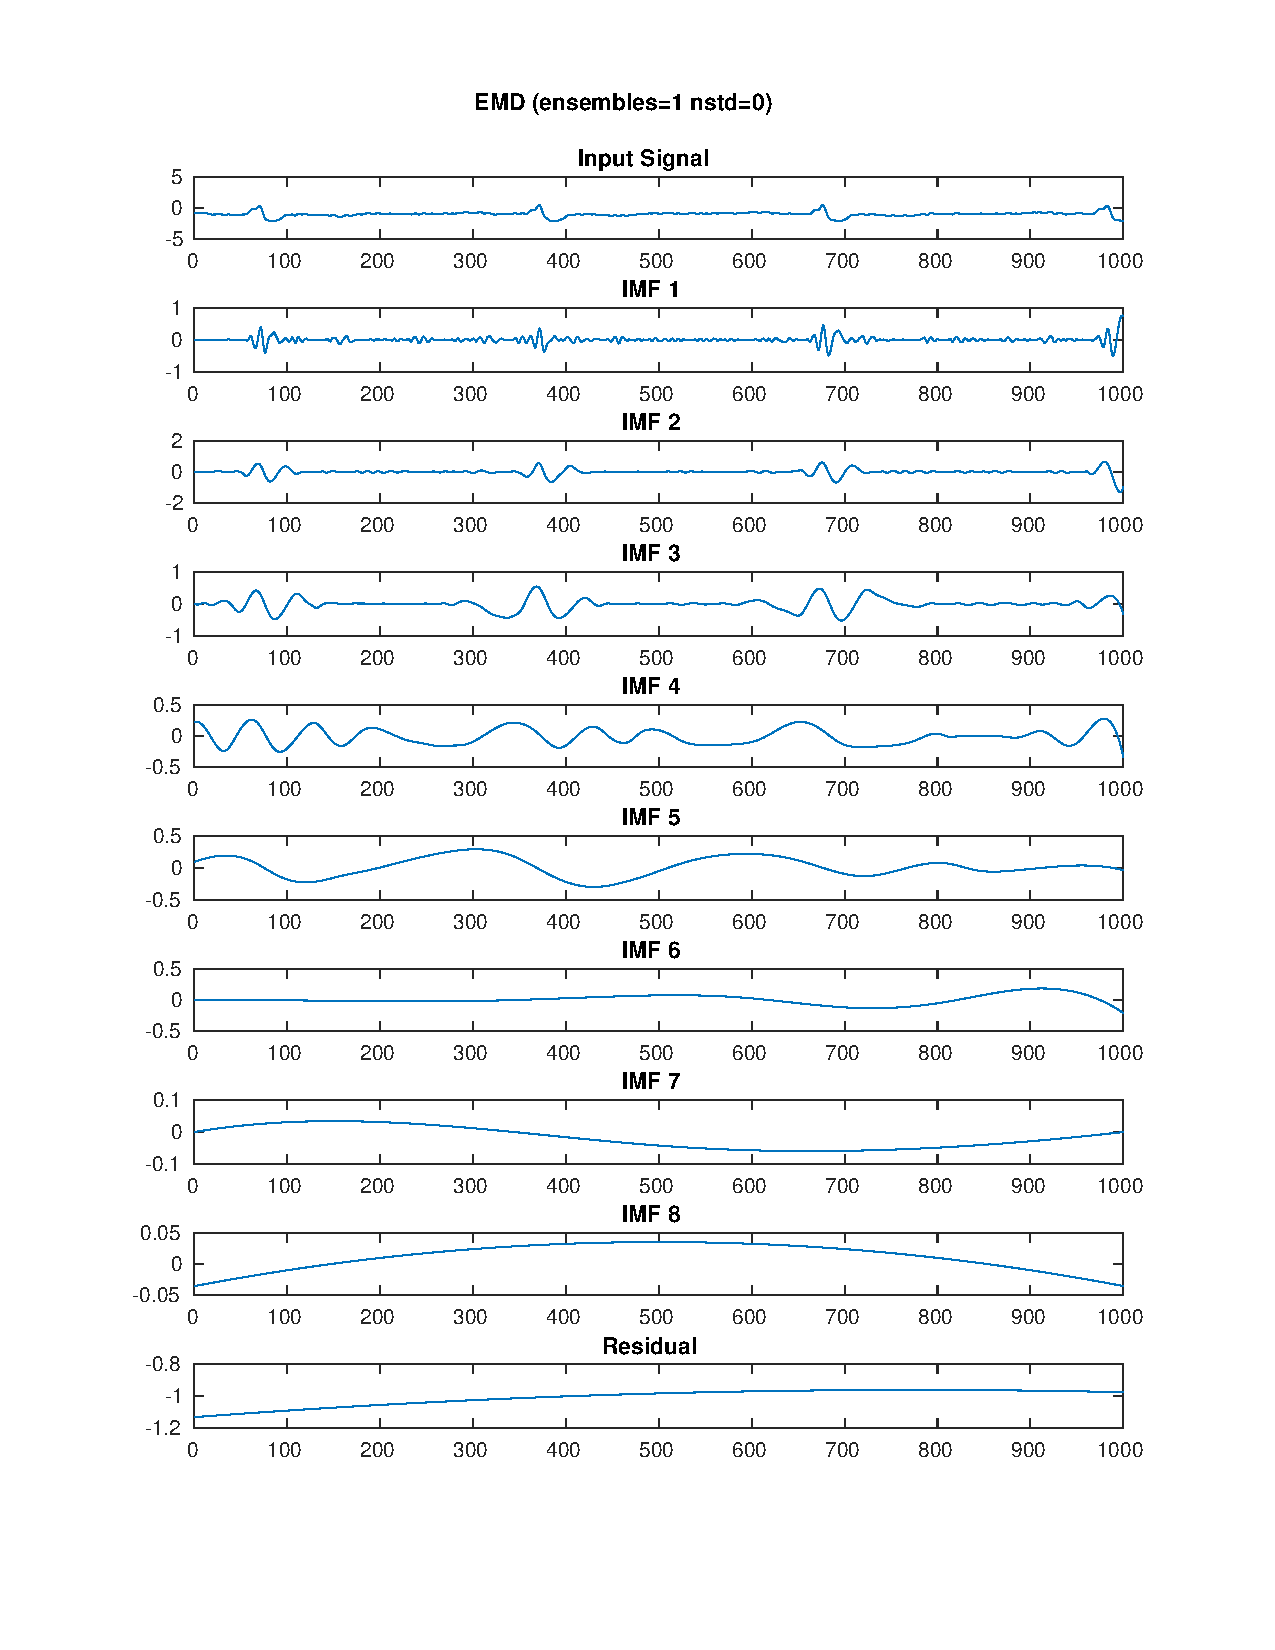
\includegraphics[width=\textwidth]{fig/118l1_emd.pdf}
\end{minipage}
\begin{minipage}{0.48\textwidth}
	\centering
	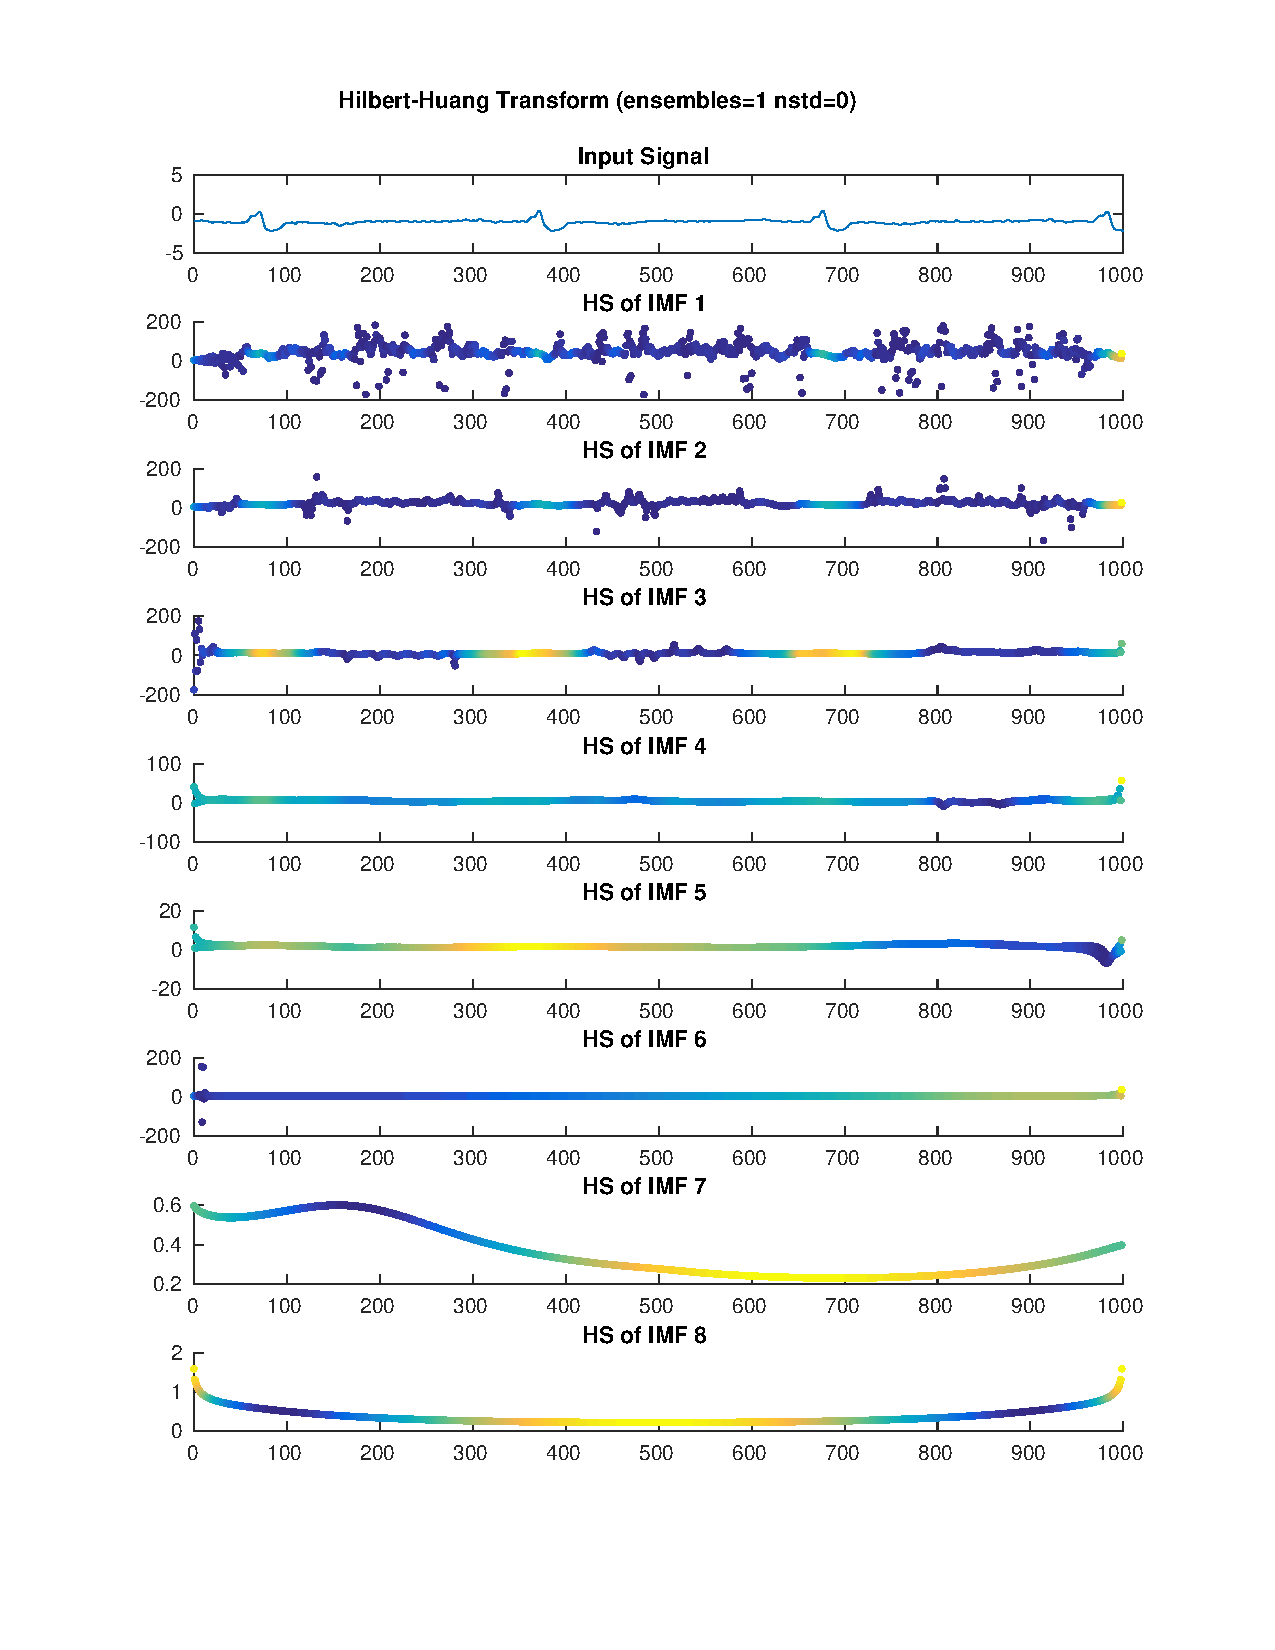
\includegraphics[width=\textwidth]{fig/118l1_hht.pdf}
\end{minipage}
\vfill
\caption{EMD και HHT του σήματος 118. Τα IMFs που μοντελοποιούν τον καρδιακό παλμό έχουν μικρότερη στιγμιαία συχνότητα από τα αντίστοιχα των ασθενών που δεν πάσχουν από RBBB.}
\label{fig:118l1_hht}
\end{figure}


% --- EEMD/HHT ---
\begin{figure}[H]
\centering
\begin{minipage}{0.48\textwidth}
	\centering
	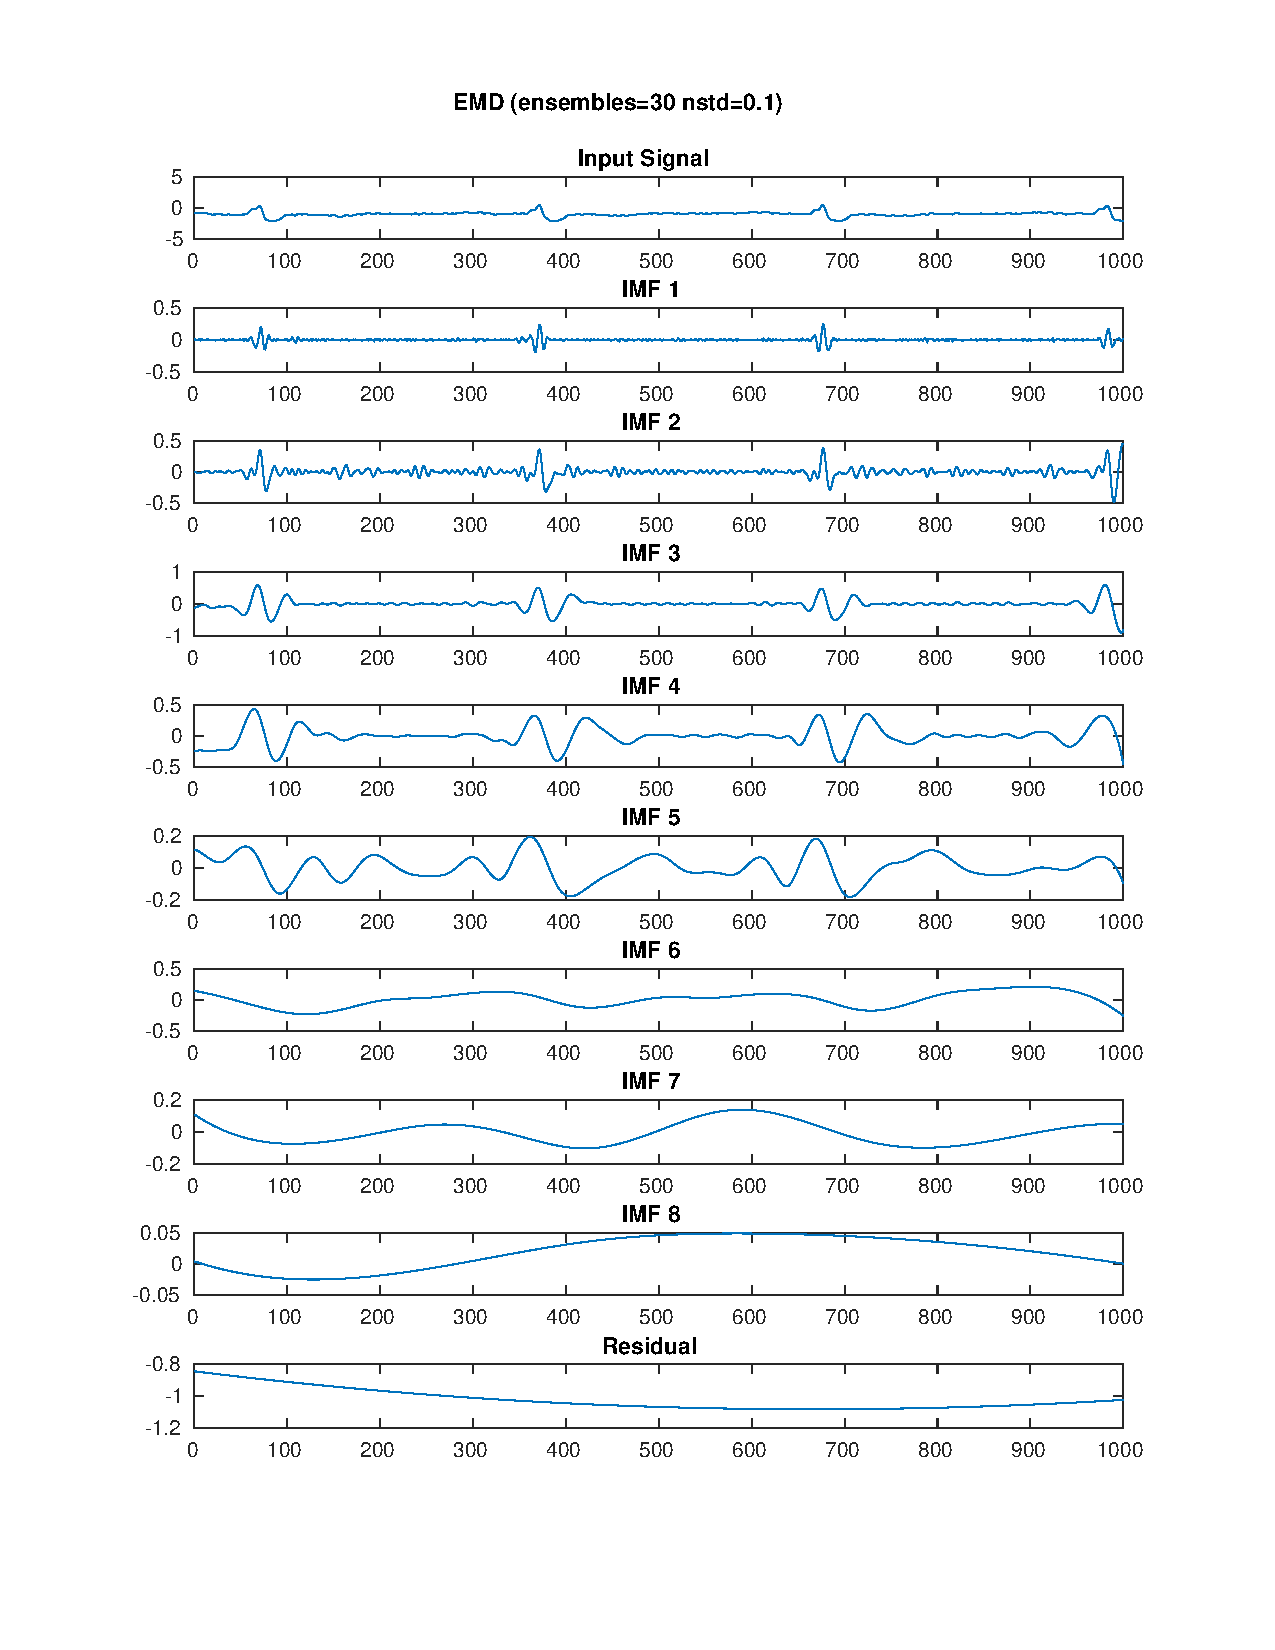
\includegraphics[width=\textwidth]{fig/118l1_emd_ensemble.pdf}
\end{minipage}
\begin{minipage}{0.48\textwidth}
	\centering
	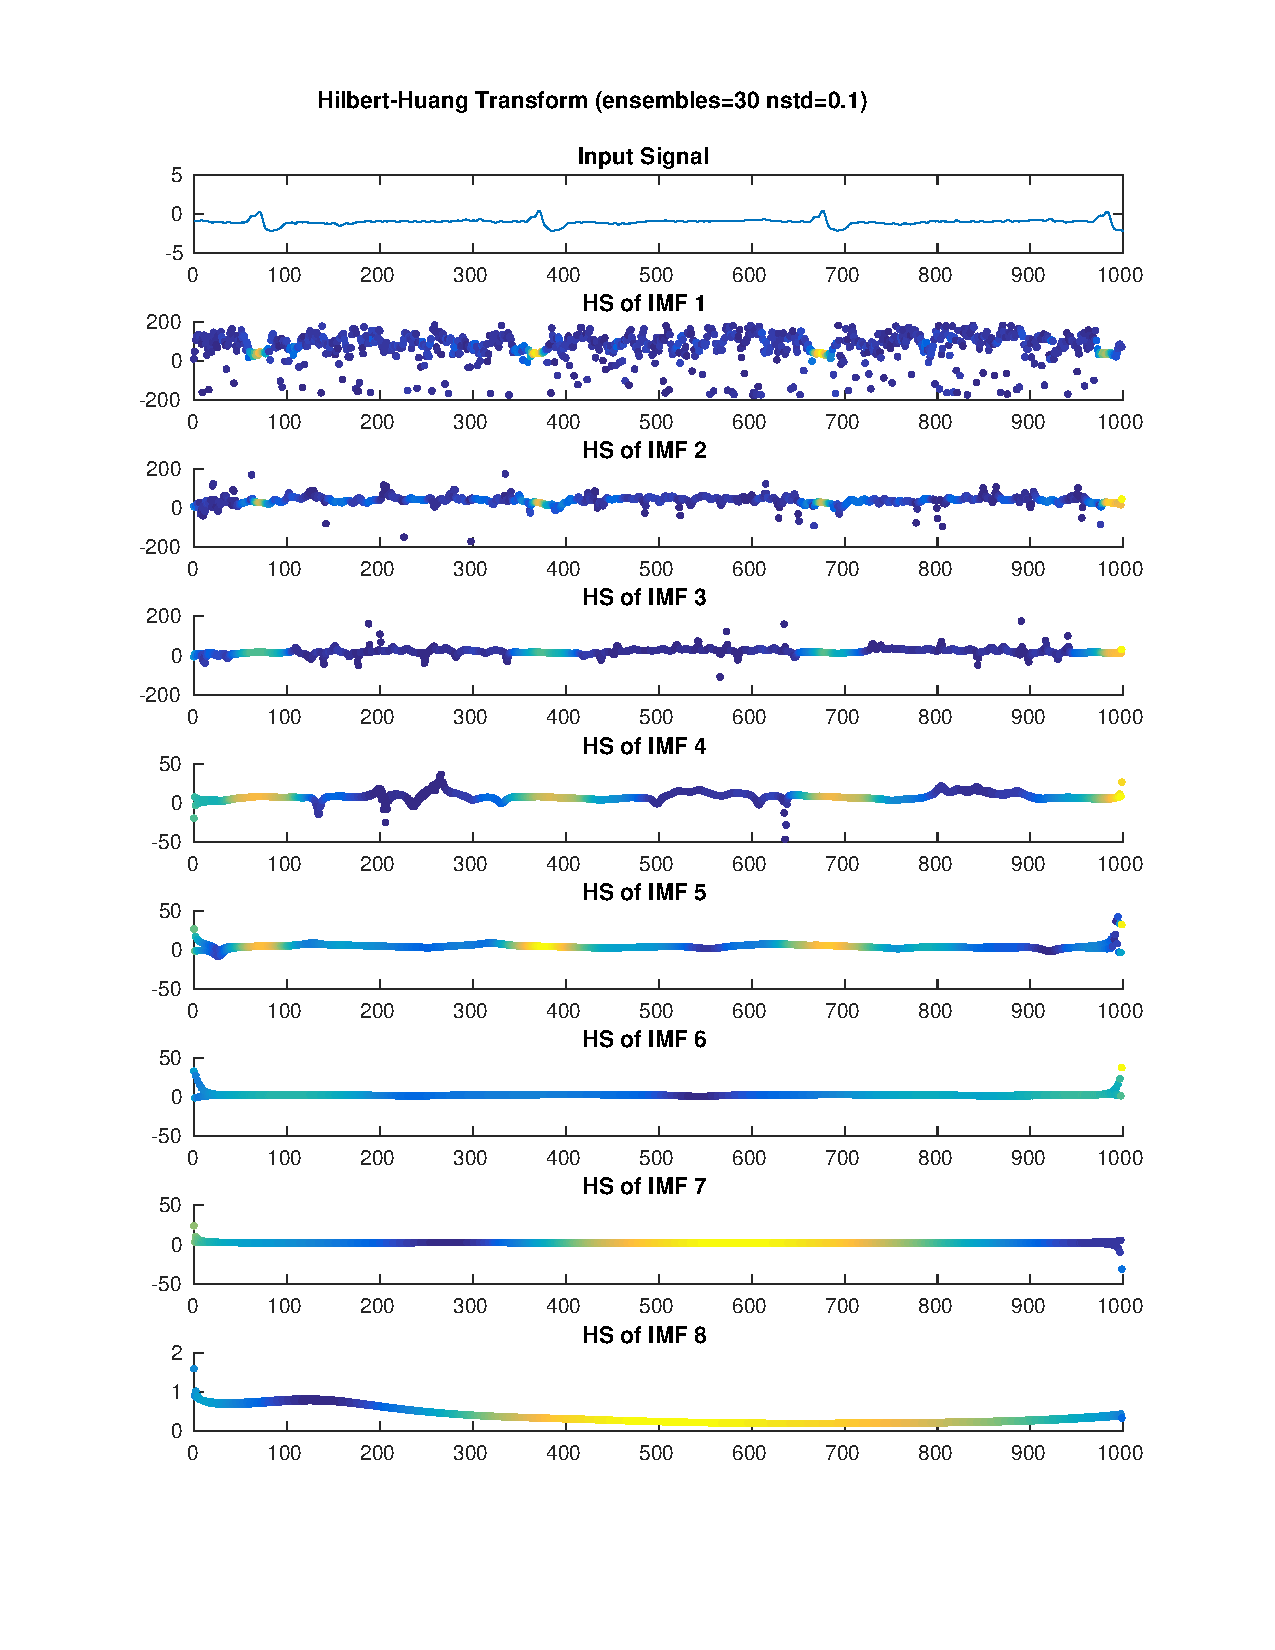
\includegraphics[width=\textwidth]{fig/118l1_hht_ensemble.pdf}
\end{minipage}
\vfill
\caption{EEMD και HHT με $n_{ens}=100$ και $\sigma_n = 0.1$. Η μείωση του mode mixing μεταξύ των IMFs, μας επιτρέπει να παρατηρήσουμε ευκολότερα τη διαφορά των στιγμιαίων συχνοτήτων που περιγράψαμε παραπάνω.}
\label{fig:118l1_hht_ensemble}
\end{figure}


\subsubsection*{Σήμα 217}

% --- STFT, WDF, CWT ---
\begin{figure}[H]
\centering
\begin{minipage}{0.48\textwidth}
	\centering
	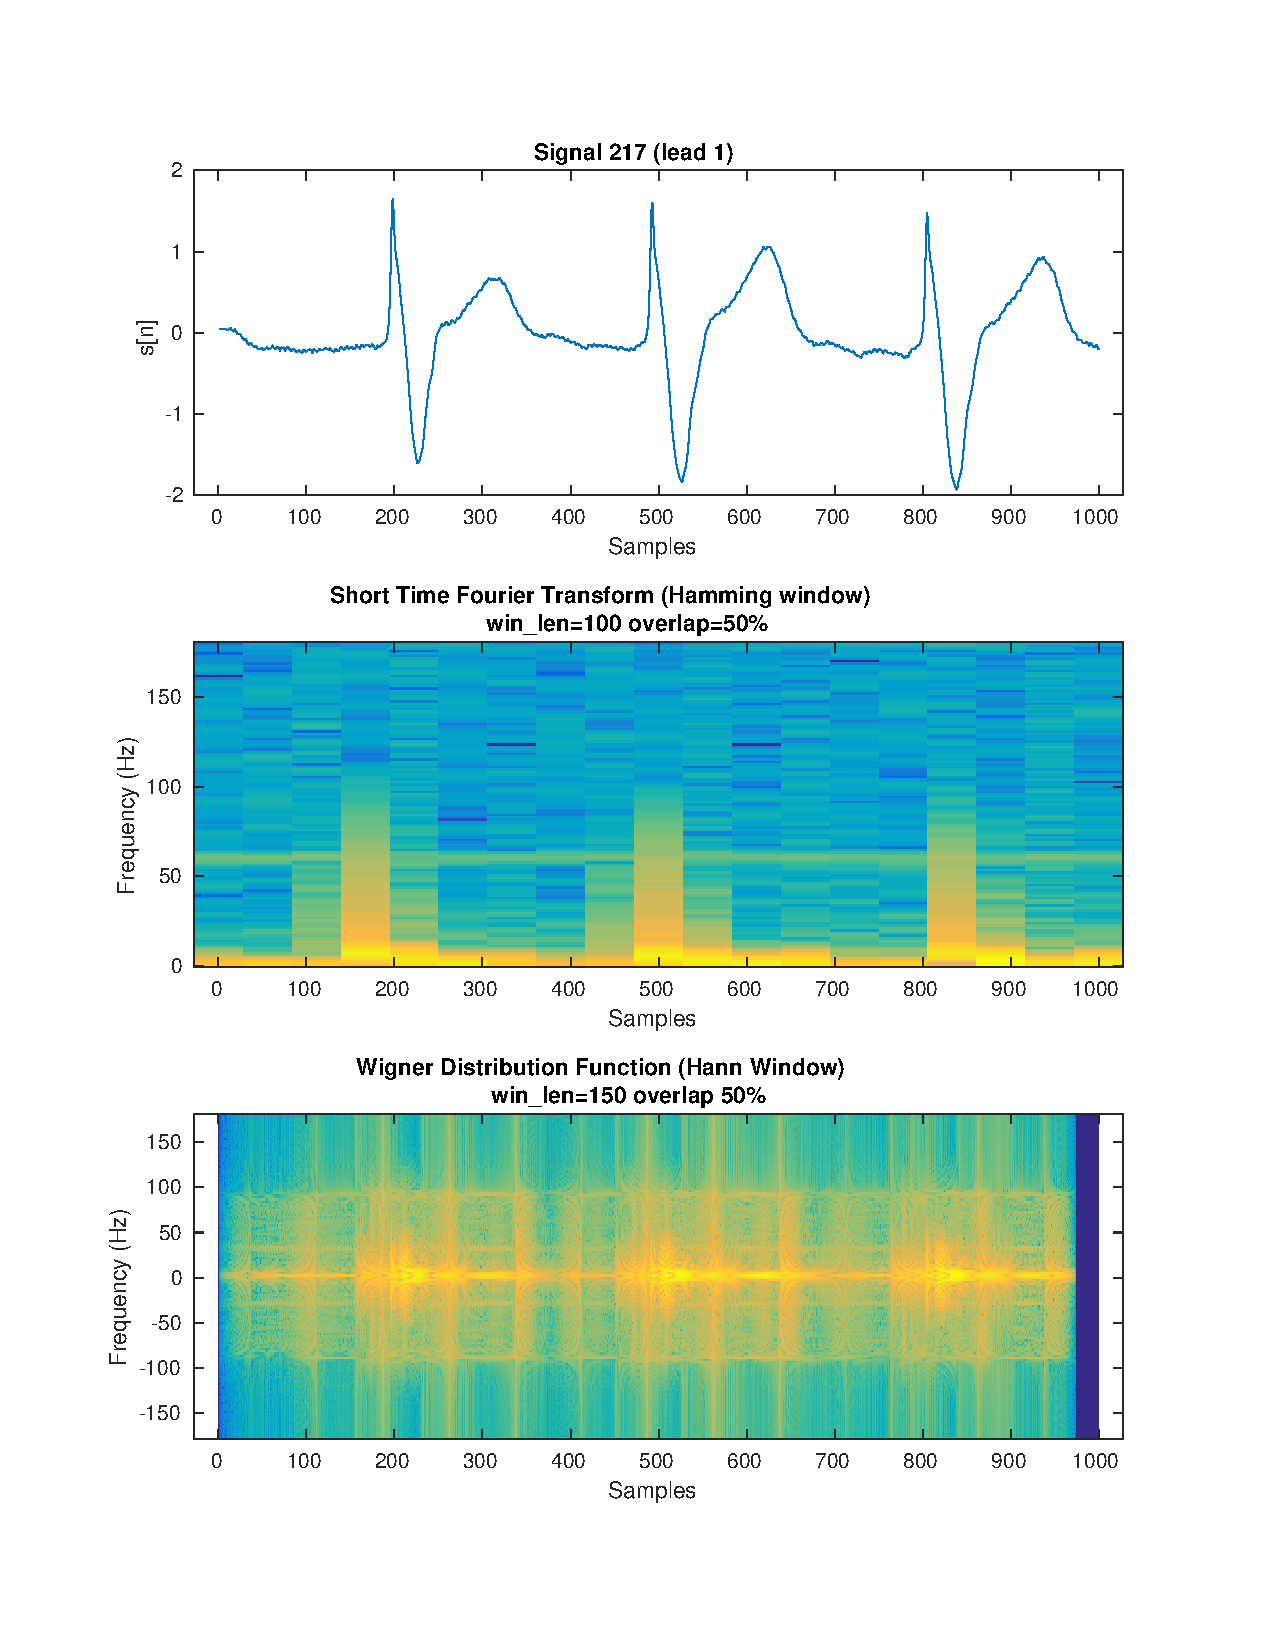
\includegraphics[width=\textwidth]{fig/217l1_stft_wdf.pdf}
\end{minipage}
\begin{minipage}{0.48\textwidth}
	\centering
	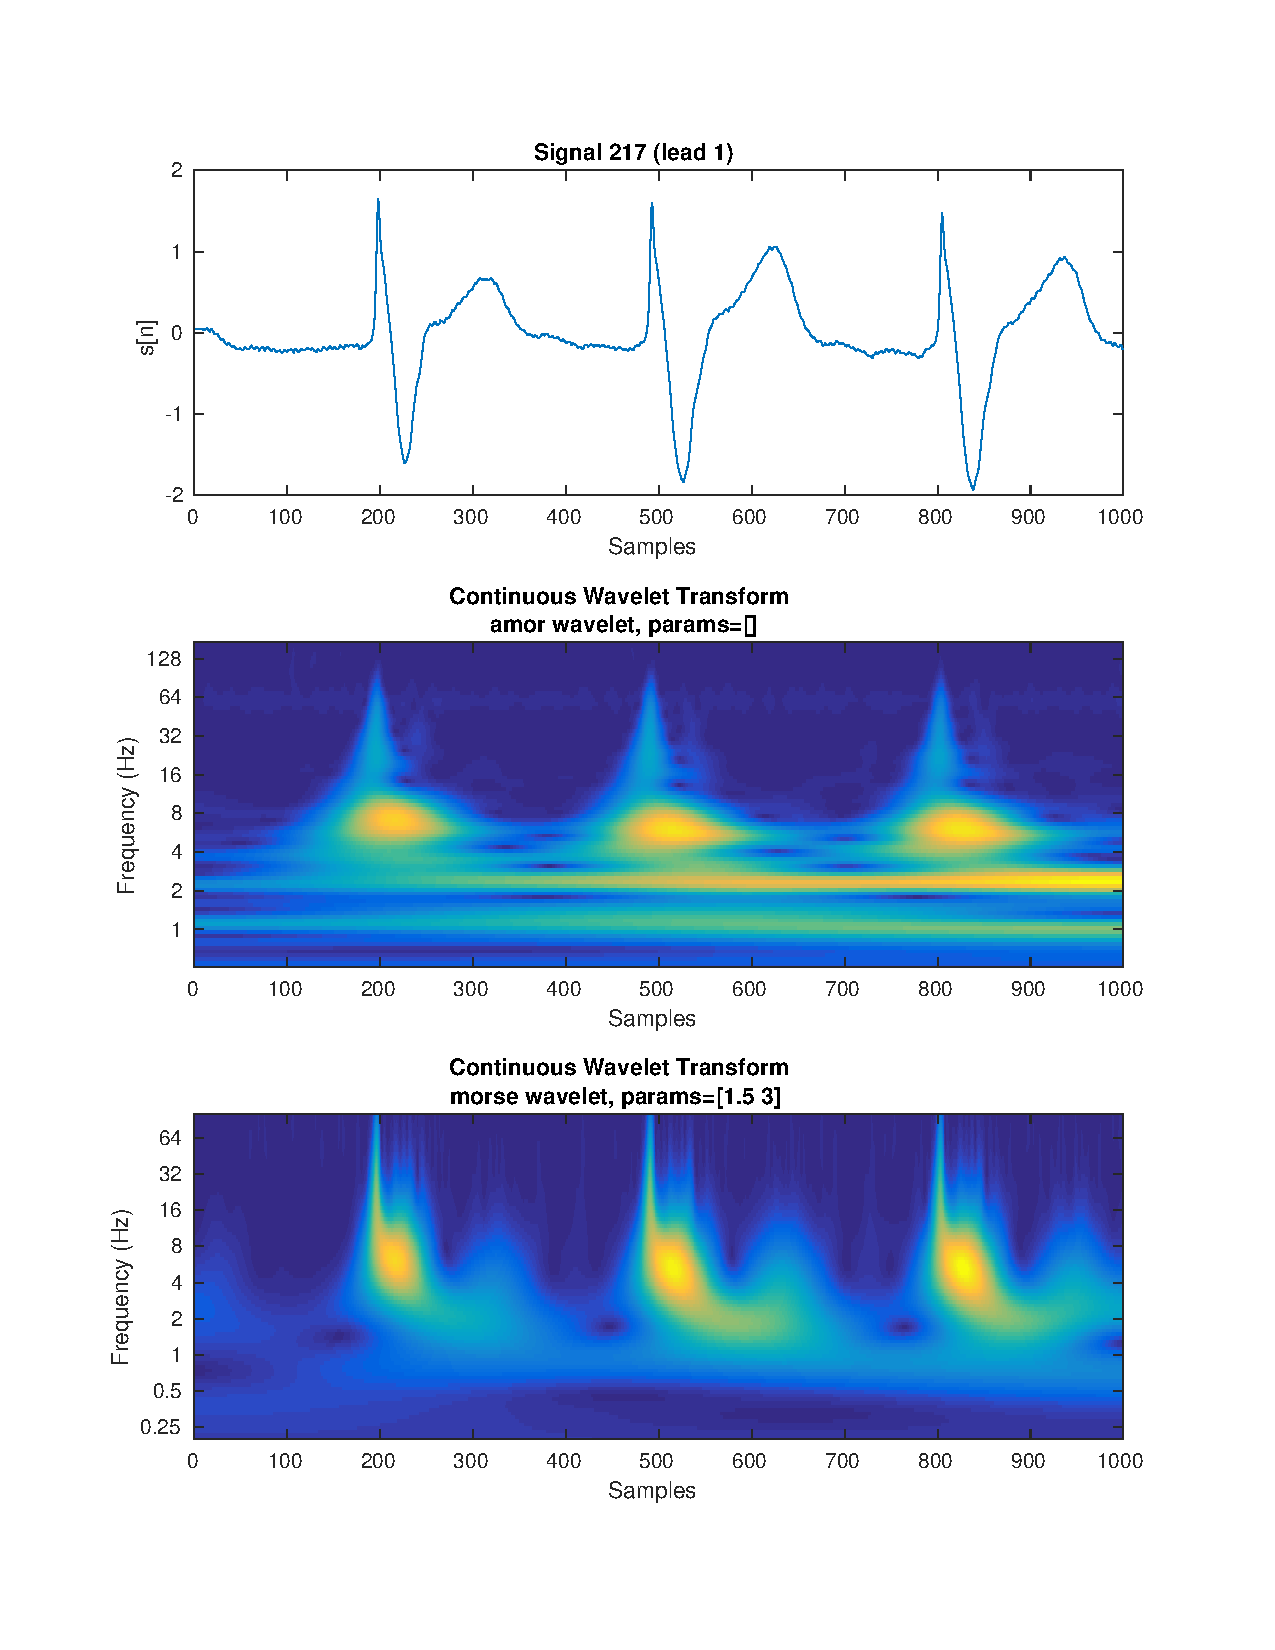
\includegraphics[width=\textwidth]{fig/217l1_cwt.pdf}
\end{minipage}
\vfill
\caption{STFT, WDF και συνεχής Wavelet Transform του σήματος 217.}
\label{fig:217l1_stft_wdf_wt}
\end{figure}


% --- DWT ---
\begin{figure}[H]
\centering
\begin{minipage}{0.48\textwidth}
	\centering
	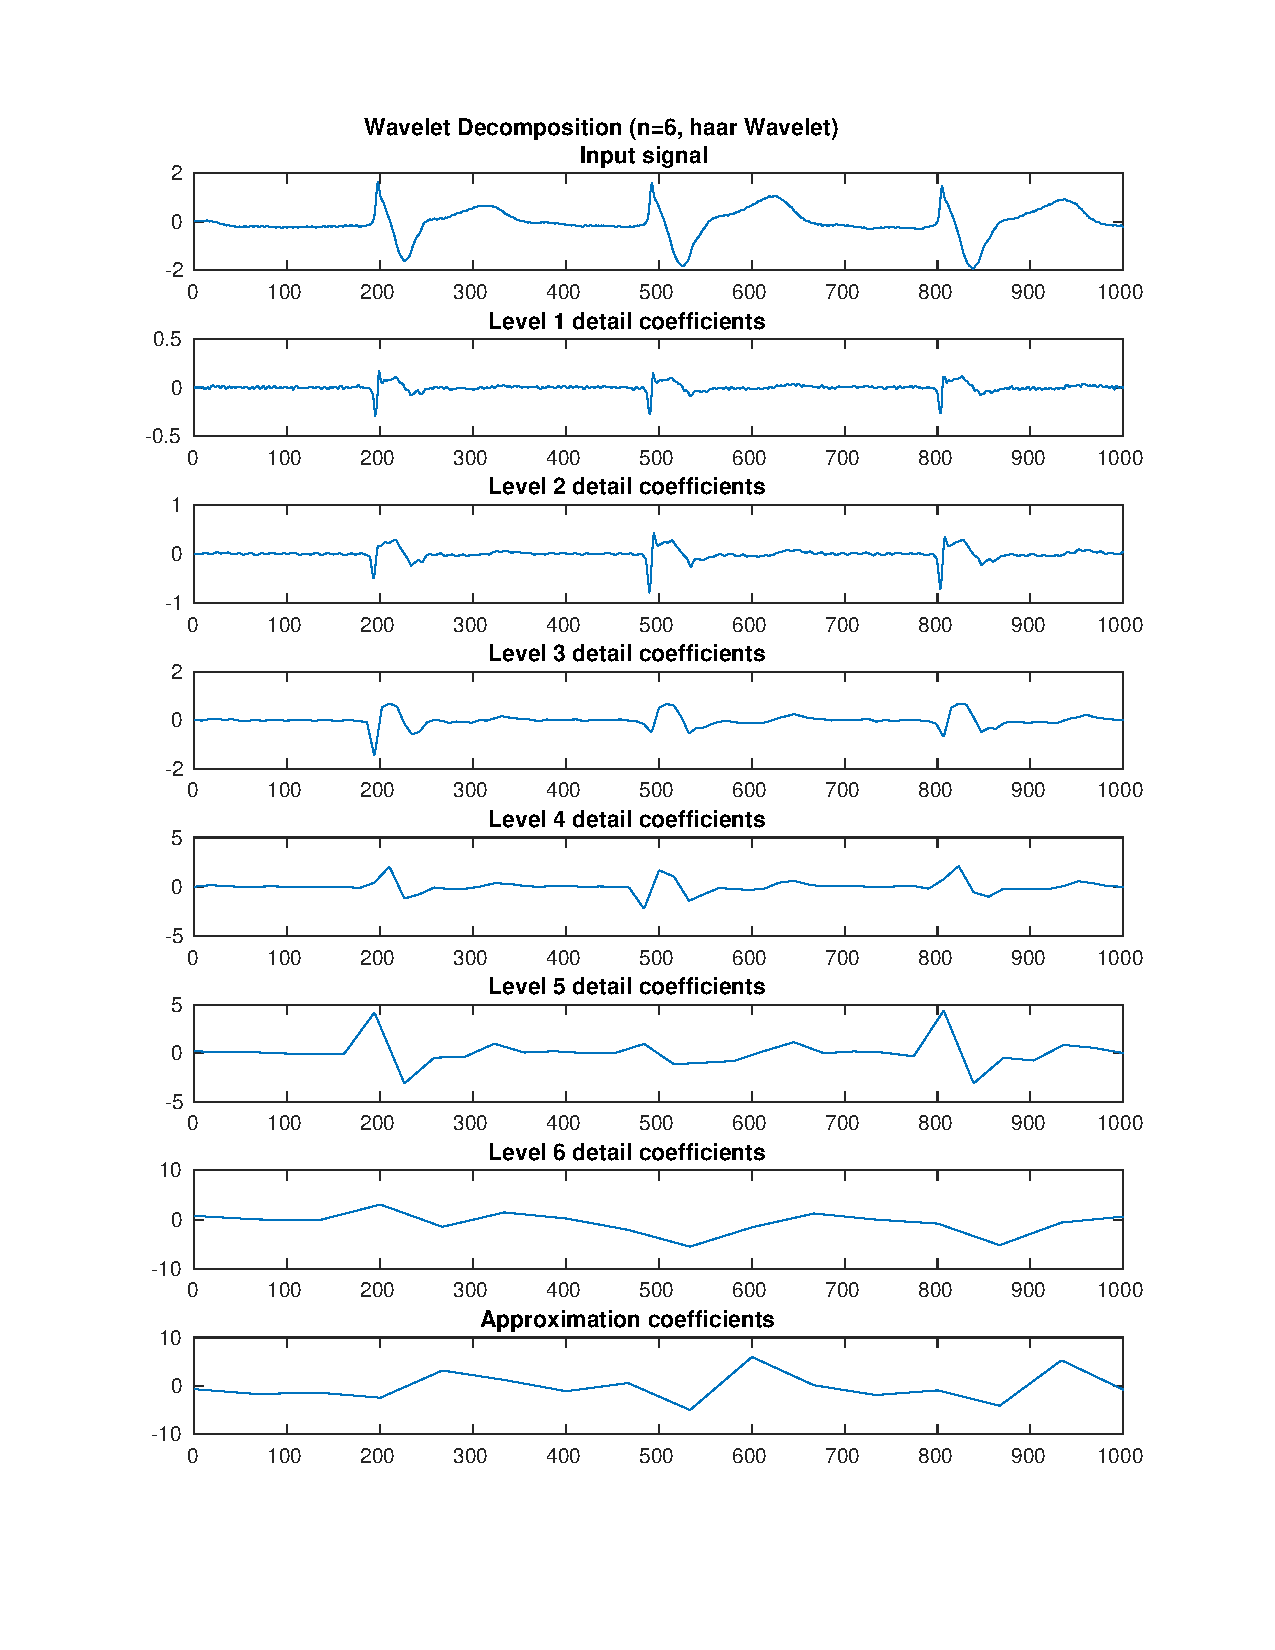
\includegraphics[width=\textwidth]{fig/217l1_dwt1.pdf}
\end{minipage}
\begin{minipage}{0.48\textwidth}
	\centering
	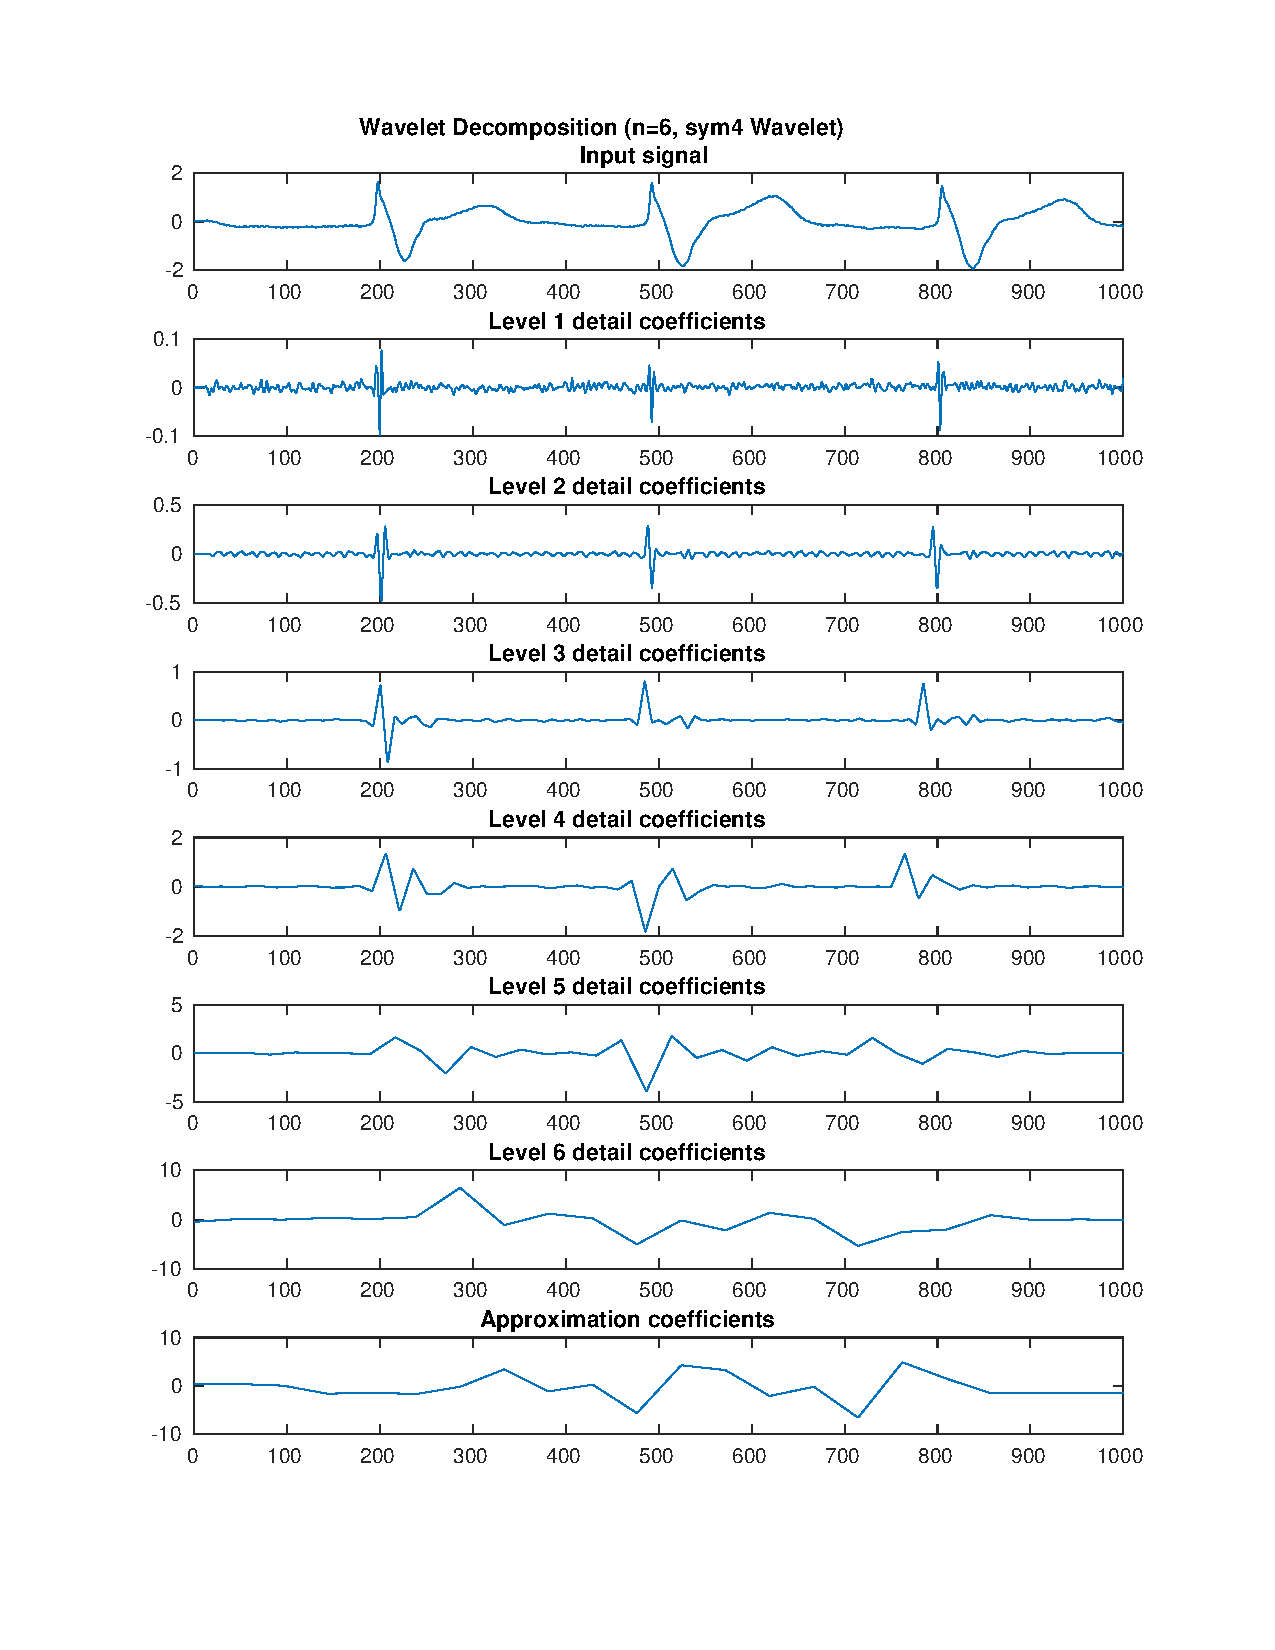
\includegraphics[width=\textwidth]{fig/217l1_dwt2.pdf}
\end{minipage}
\vfill
\caption{Διακριτός WT του σήματος χρησιμοποιώντας db4 και bior1.3.}
\label{fig:217l1_dwt}
\end{figure}


% --- EMD/HHT ---
\begin{figure}[H]
\centering
\begin{minipage}{0.48\textwidth}
	\centering
	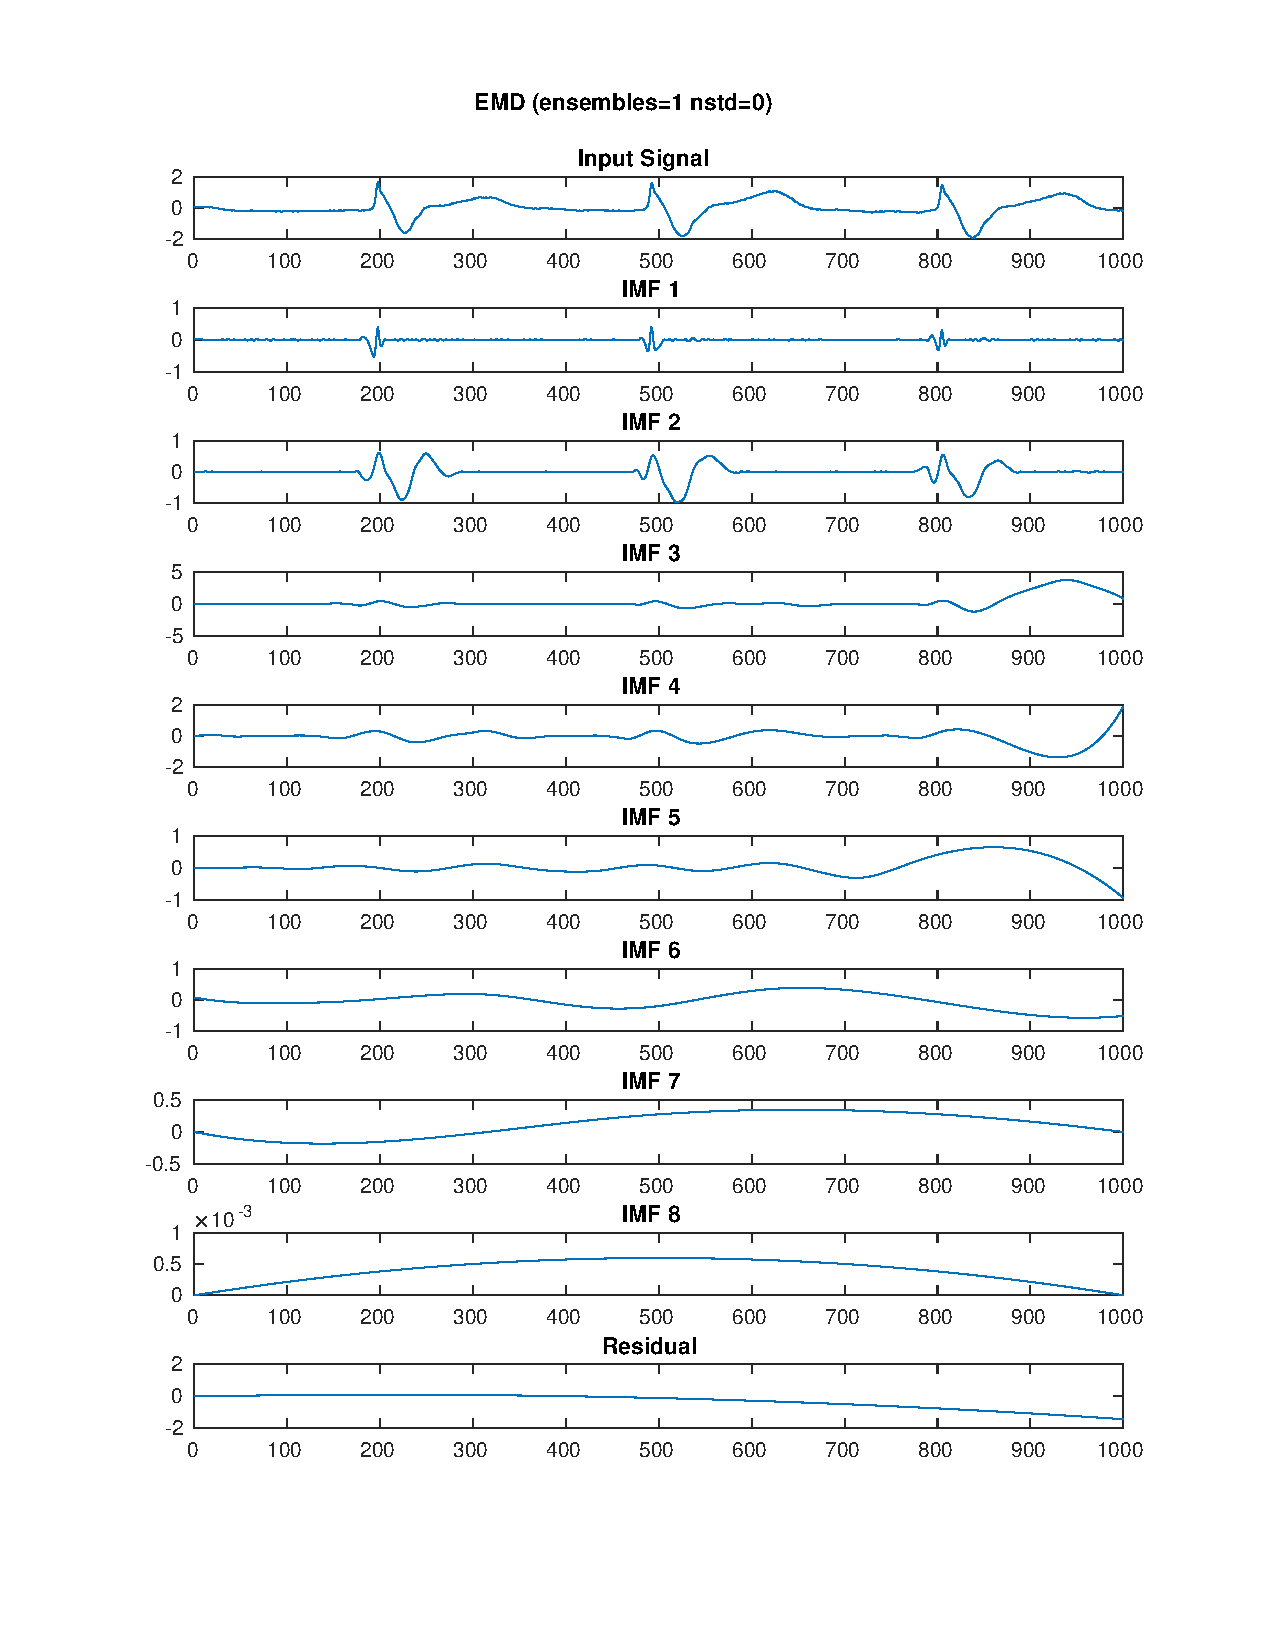
\includegraphics[width=\textwidth]{fig/217l1_emd.pdf}
\end{minipage}
\begin{minipage}{0.48\textwidth}
	\centering
	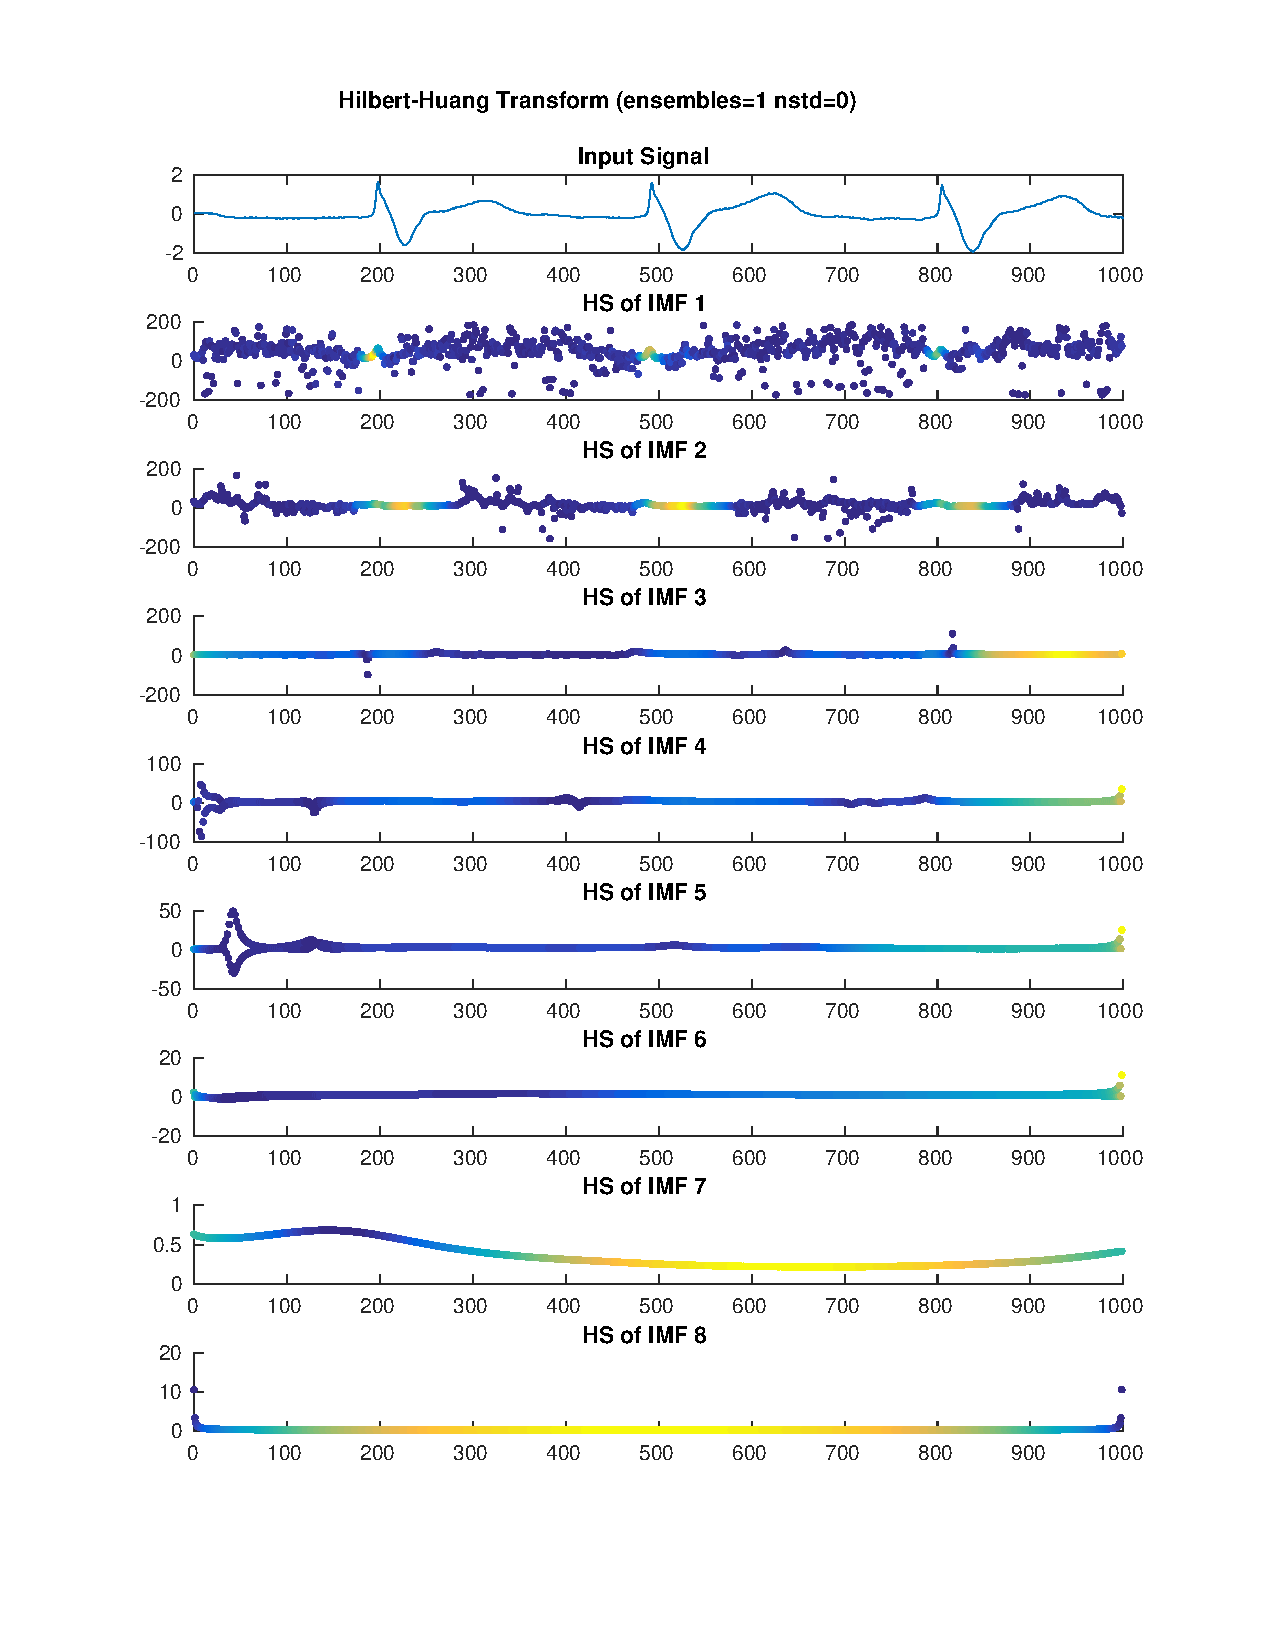
\includegraphics[width=\textwidth]{fig/217l1_hht.pdf}
\end{minipage}
\vfill
\caption{EMD και HHT του σήματος.}
\label{fig:217l1_hht}
\end{figure}


% --- EEMD/HHT ---
\begin{figure}[H]
\centering
\begin{minipage}{0.48\textwidth}
	\centering
	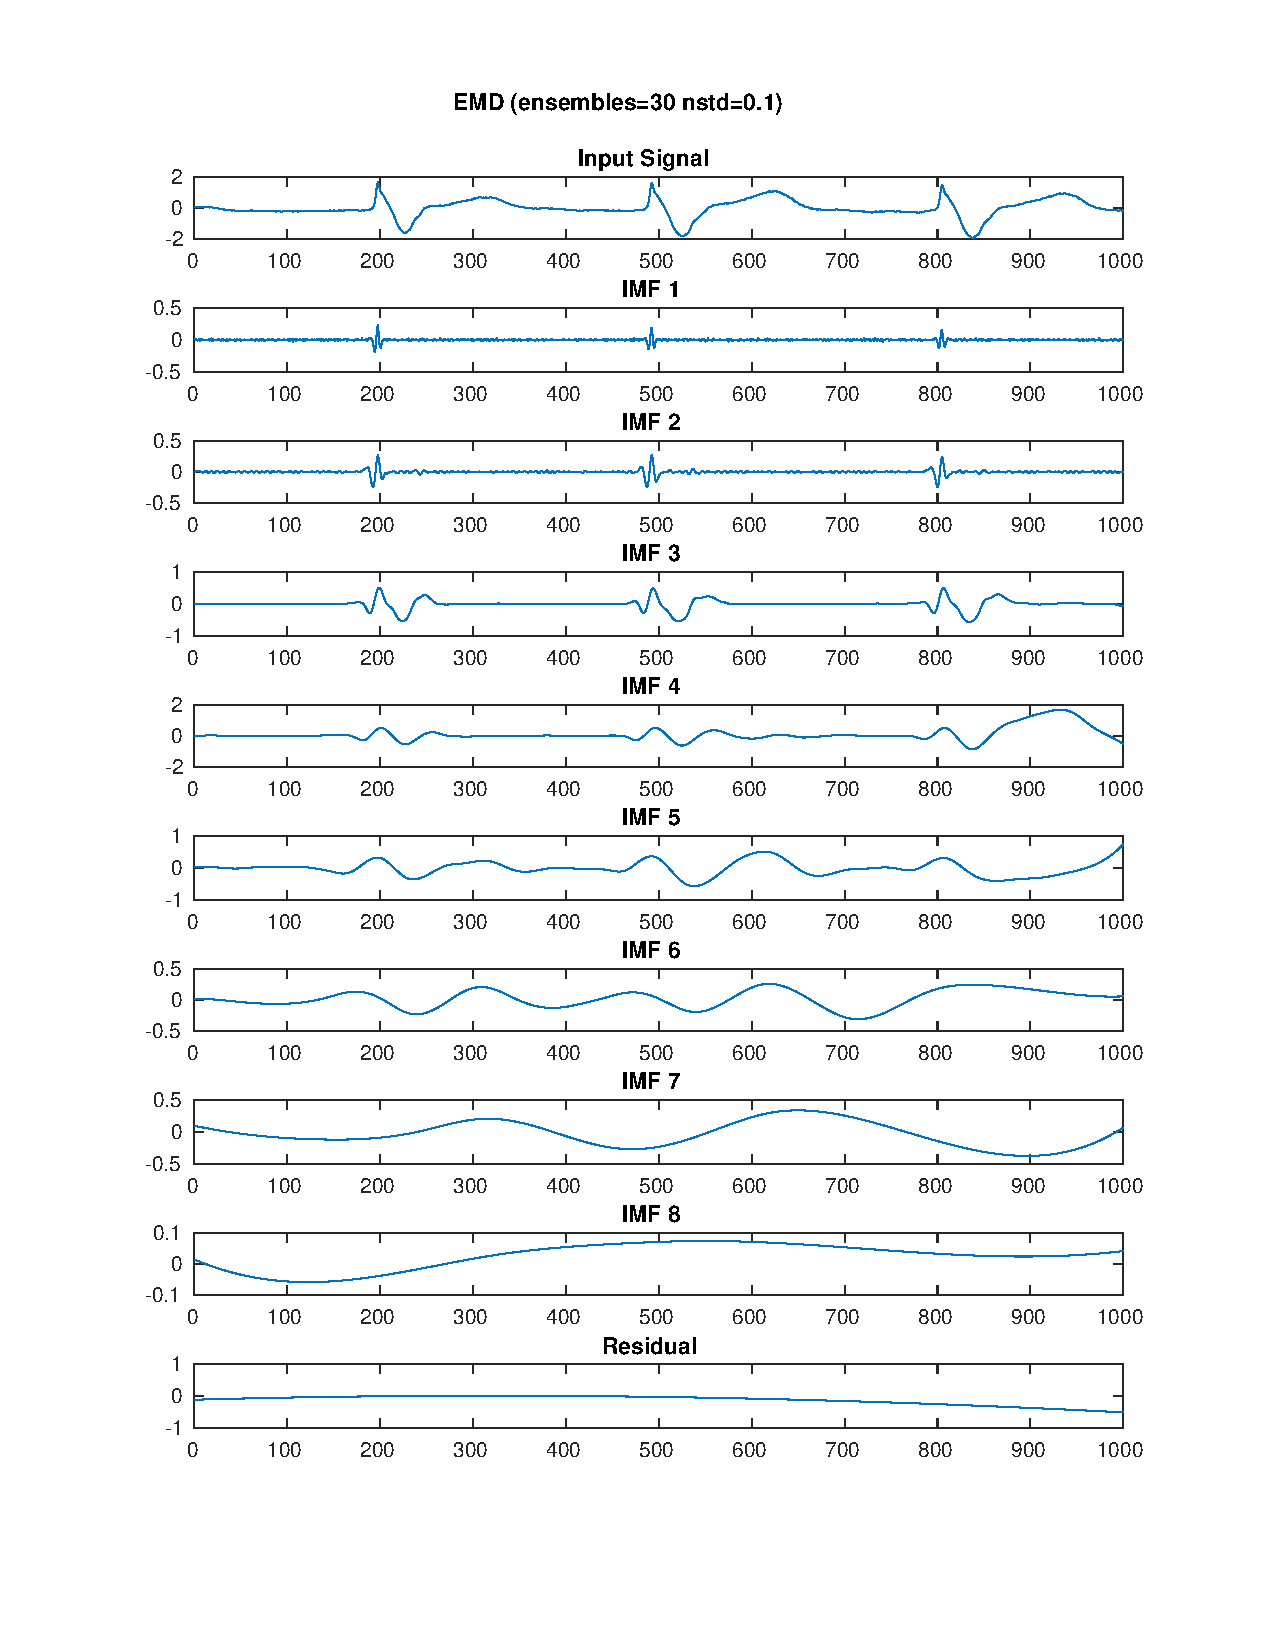
\includegraphics[width=\textwidth]{fig/217l1_emd_ensemble.pdf}
\end{minipage}
\begin{minipage}{0.48\textwidth}
	\centering
	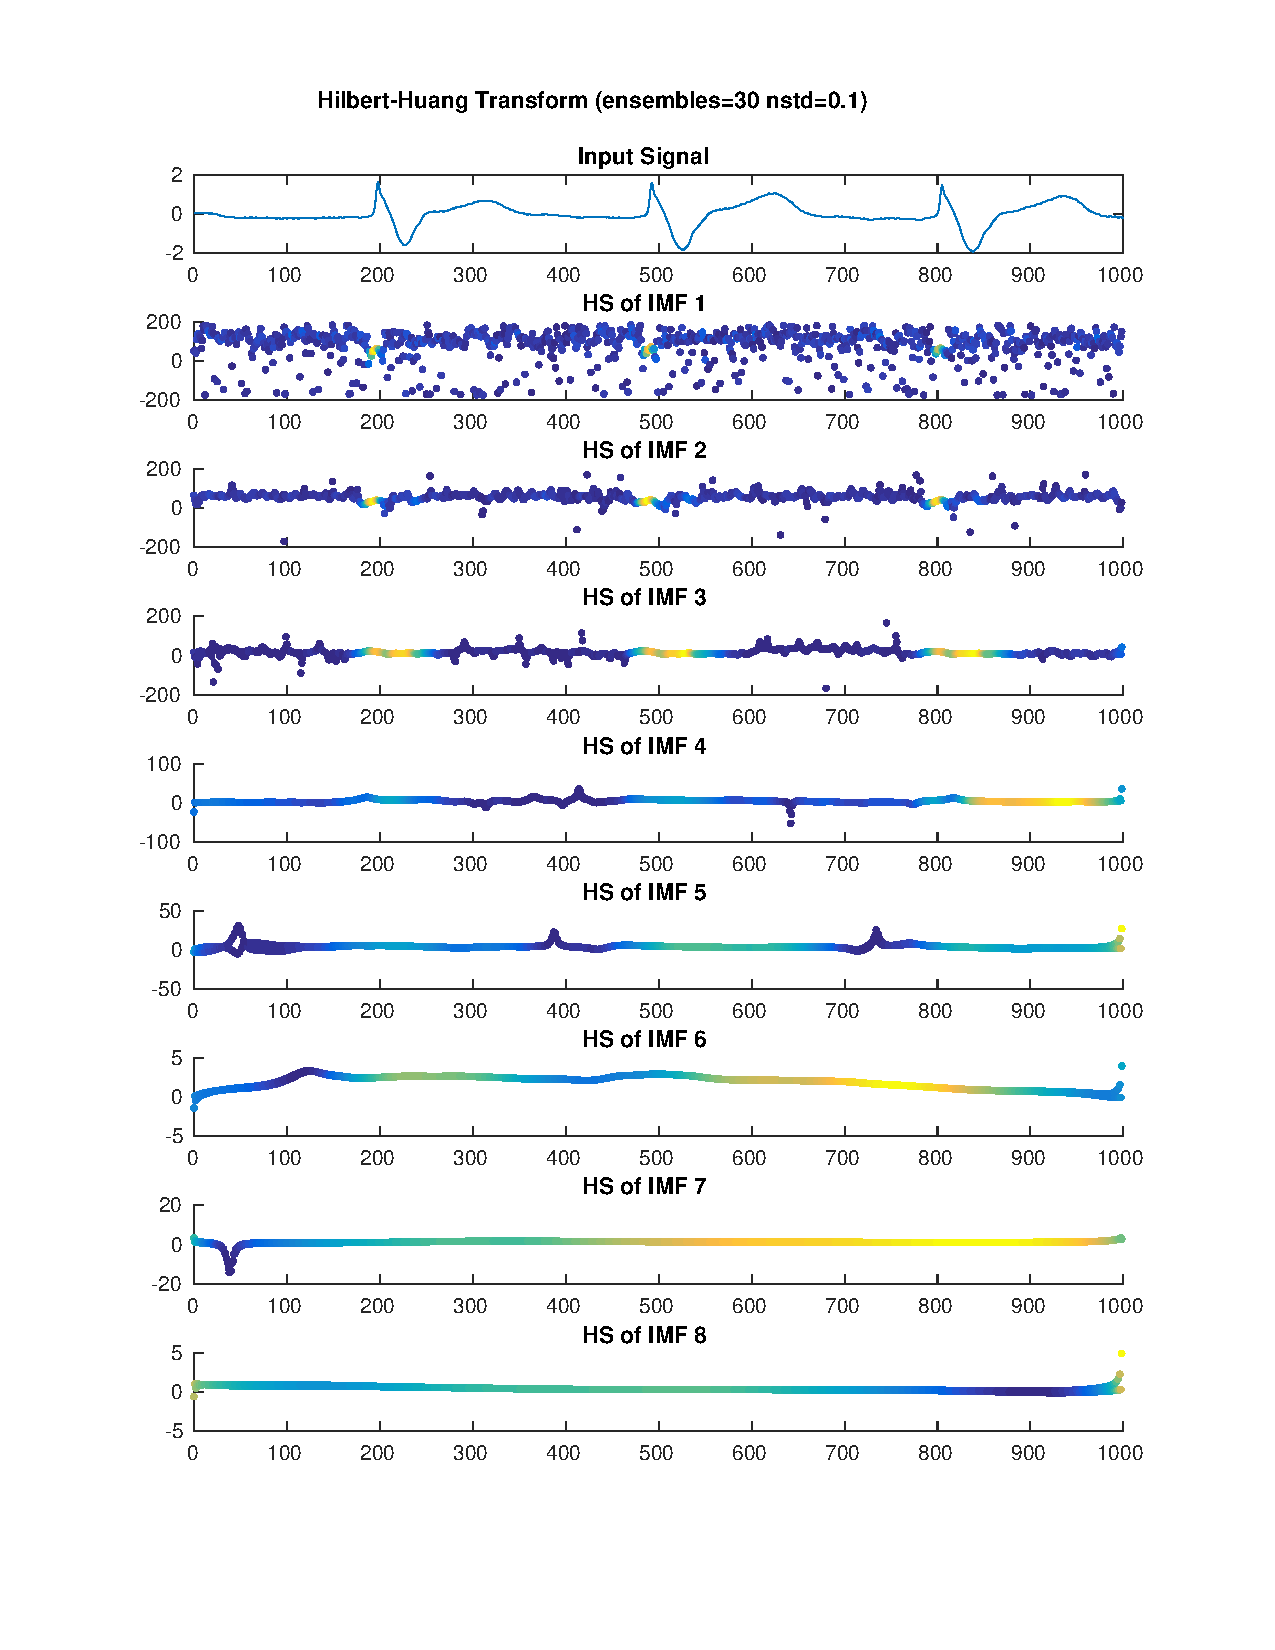
\includegraphics[width=\textwidth]{fig/217l1_hht_ensemble.pdf}
\end{minipage}
\vfill
\caption{EEMD και HHT με $n_{ens}=100$ και $\sigma_n = 0.1$.}
\label{fig:217l1_hht_ensemble}
\end{figure}

\subsubsection*{Σήμα 221}

% --- STFT, WDF, CWT ---
\begin{figure}[H]
\centering
\begin{minipage}{0.48\textwidth}
	\centering
	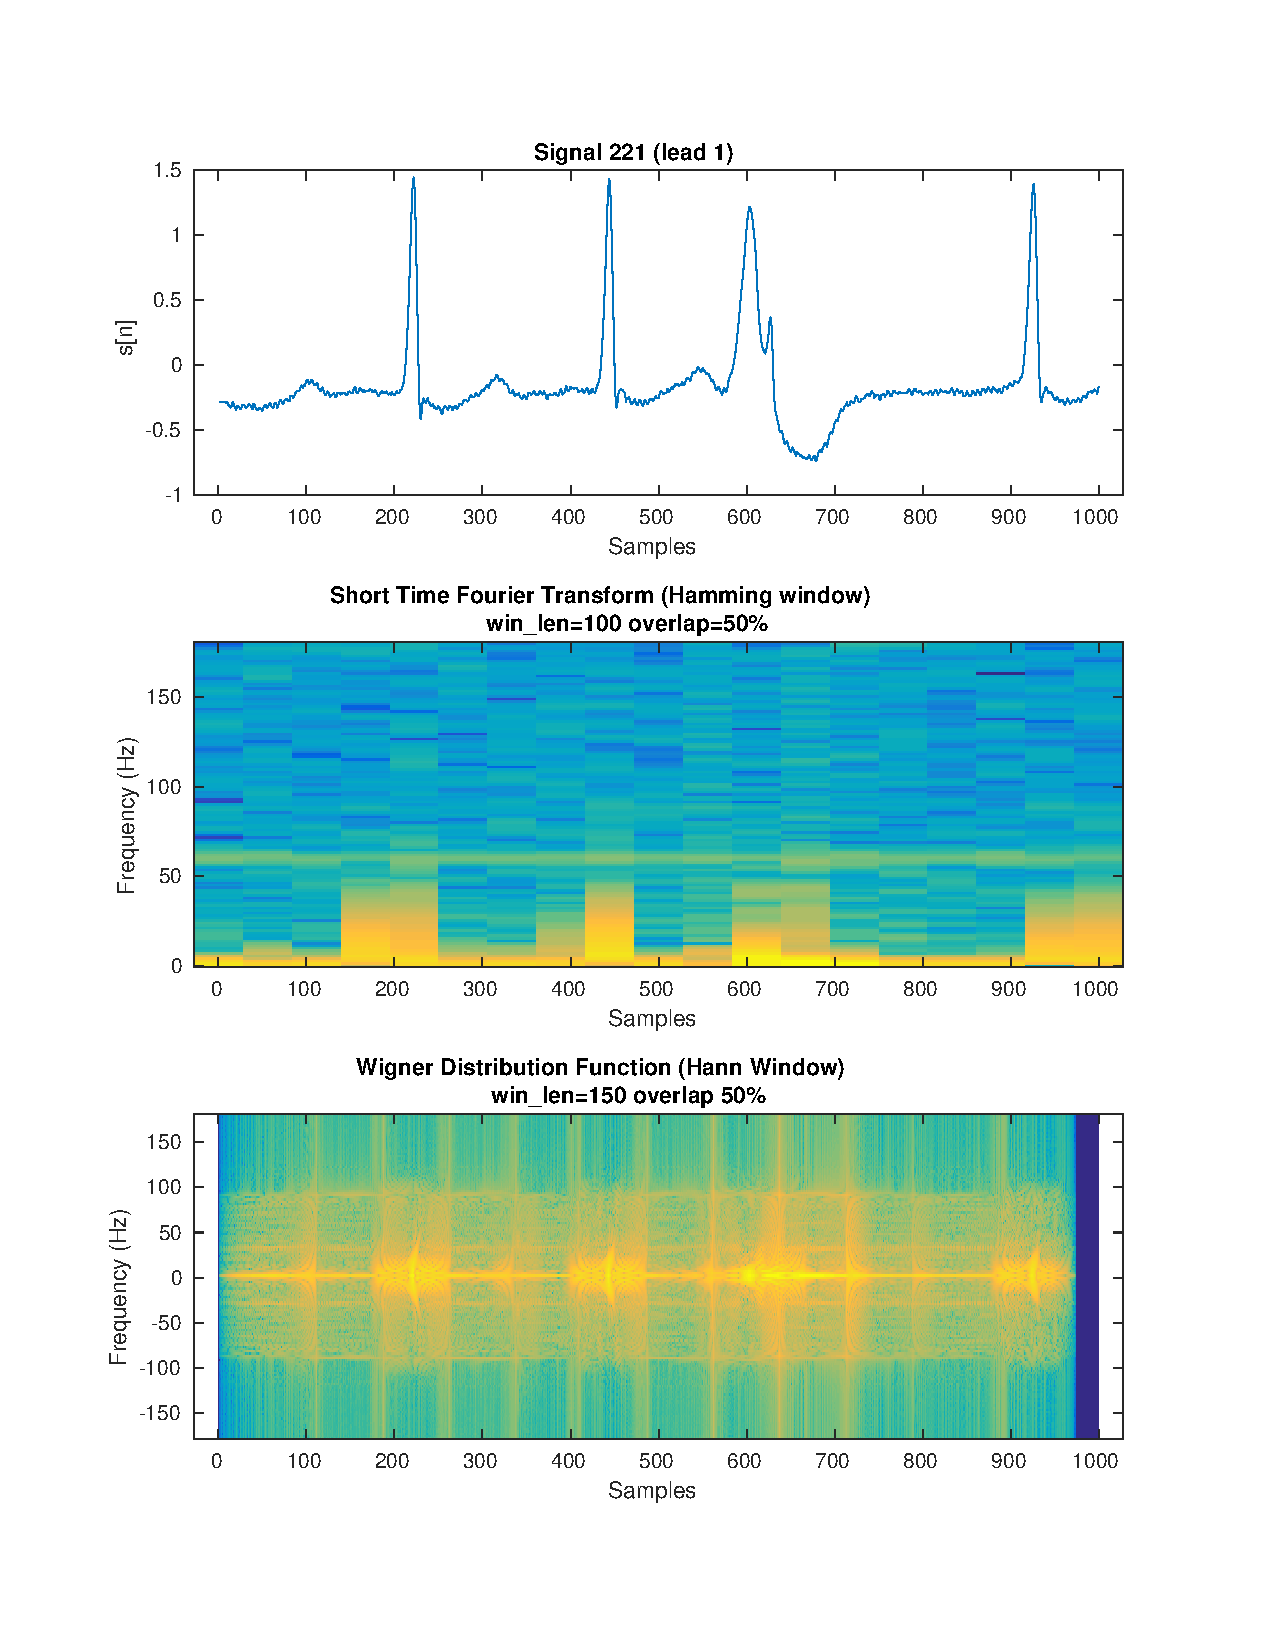
\includegraphics[width=\textwidth]{fig/221l1_stft_wdf.pdf}
\end{minipage}
\begin{minipage}{0.48\textwidth}
	\centering
	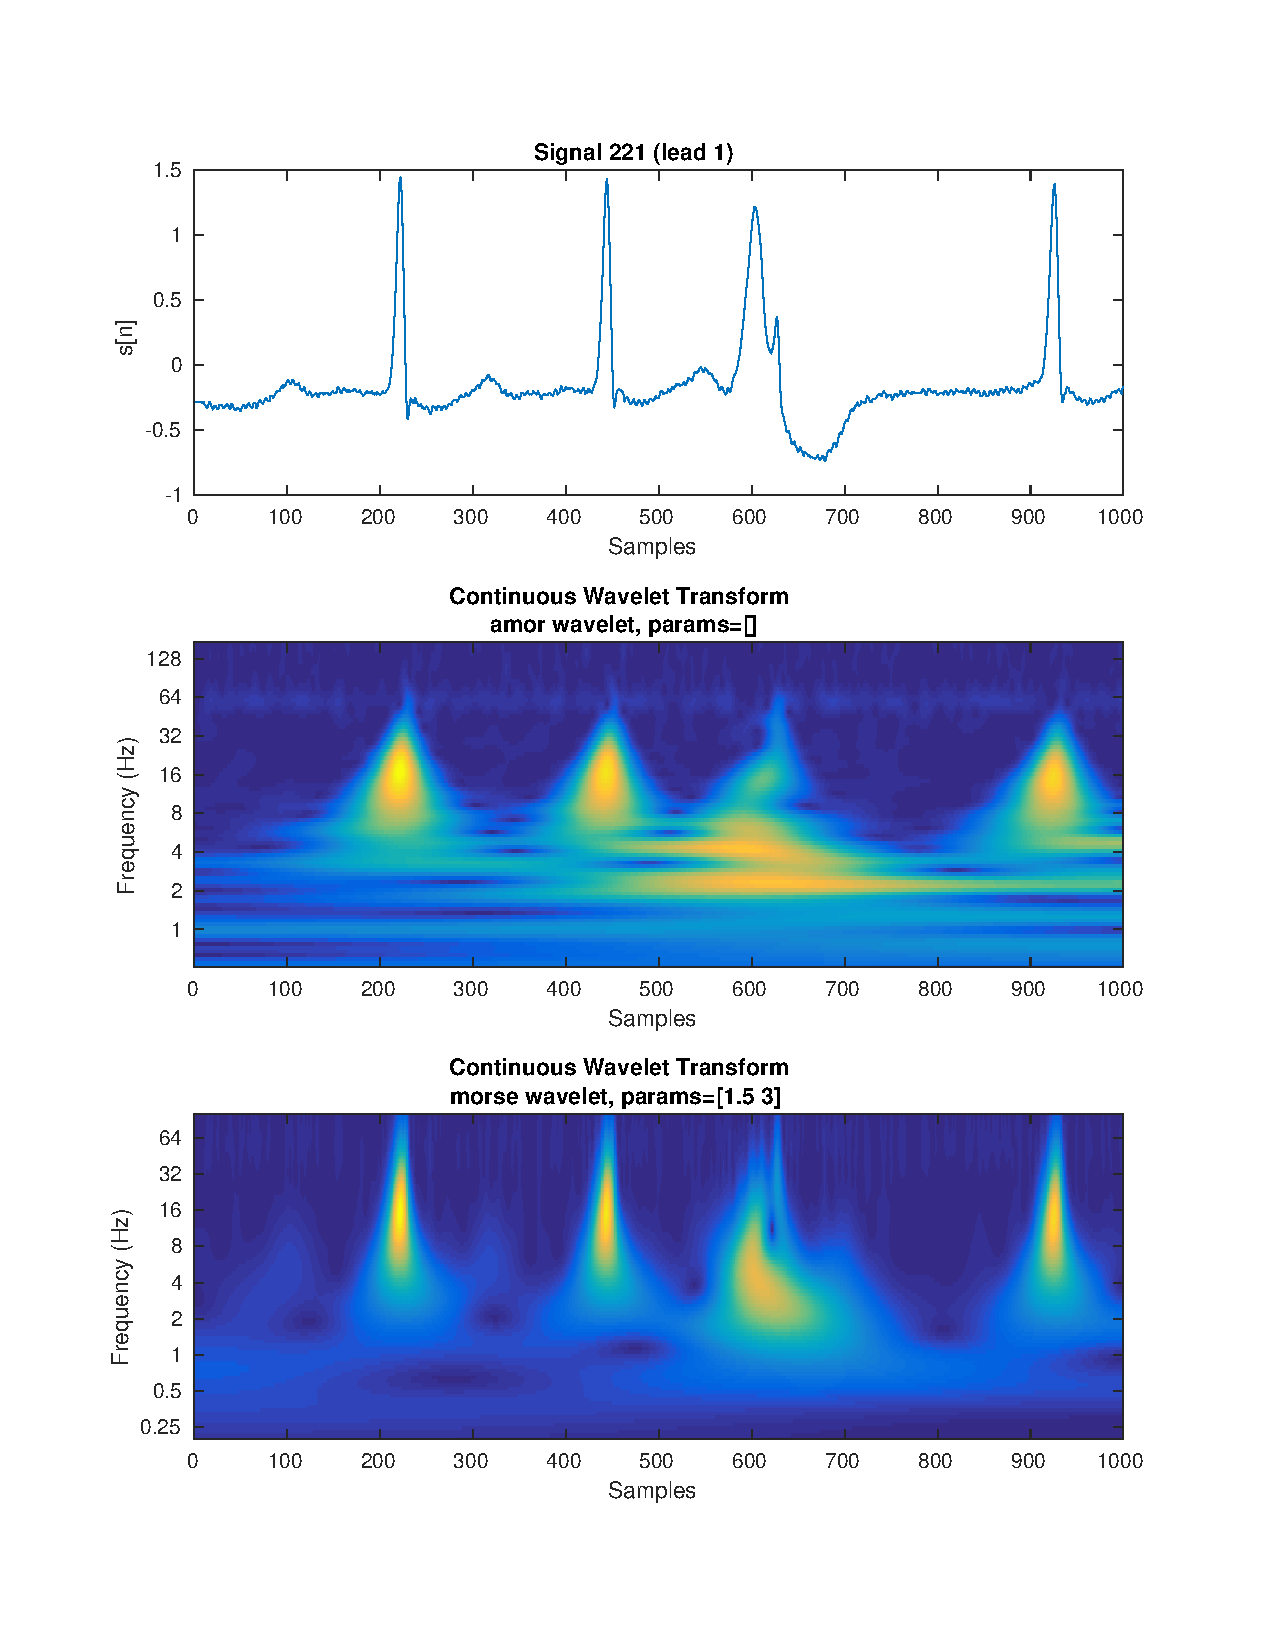
\includegraphics[width=\textwidth]{fig/221l1_cwt.pdf}
\end{minipage}
\vfill
\caption{STFT, WDF και συνεχής WT του σήματος 221.}
\label{fig:221l1_stft_wdf_wt}
\end{figure}


% --- DWT ---
\begin{figure}[H]
\centering
\begin{minipage}{0.48\textwidth}
	\centering
	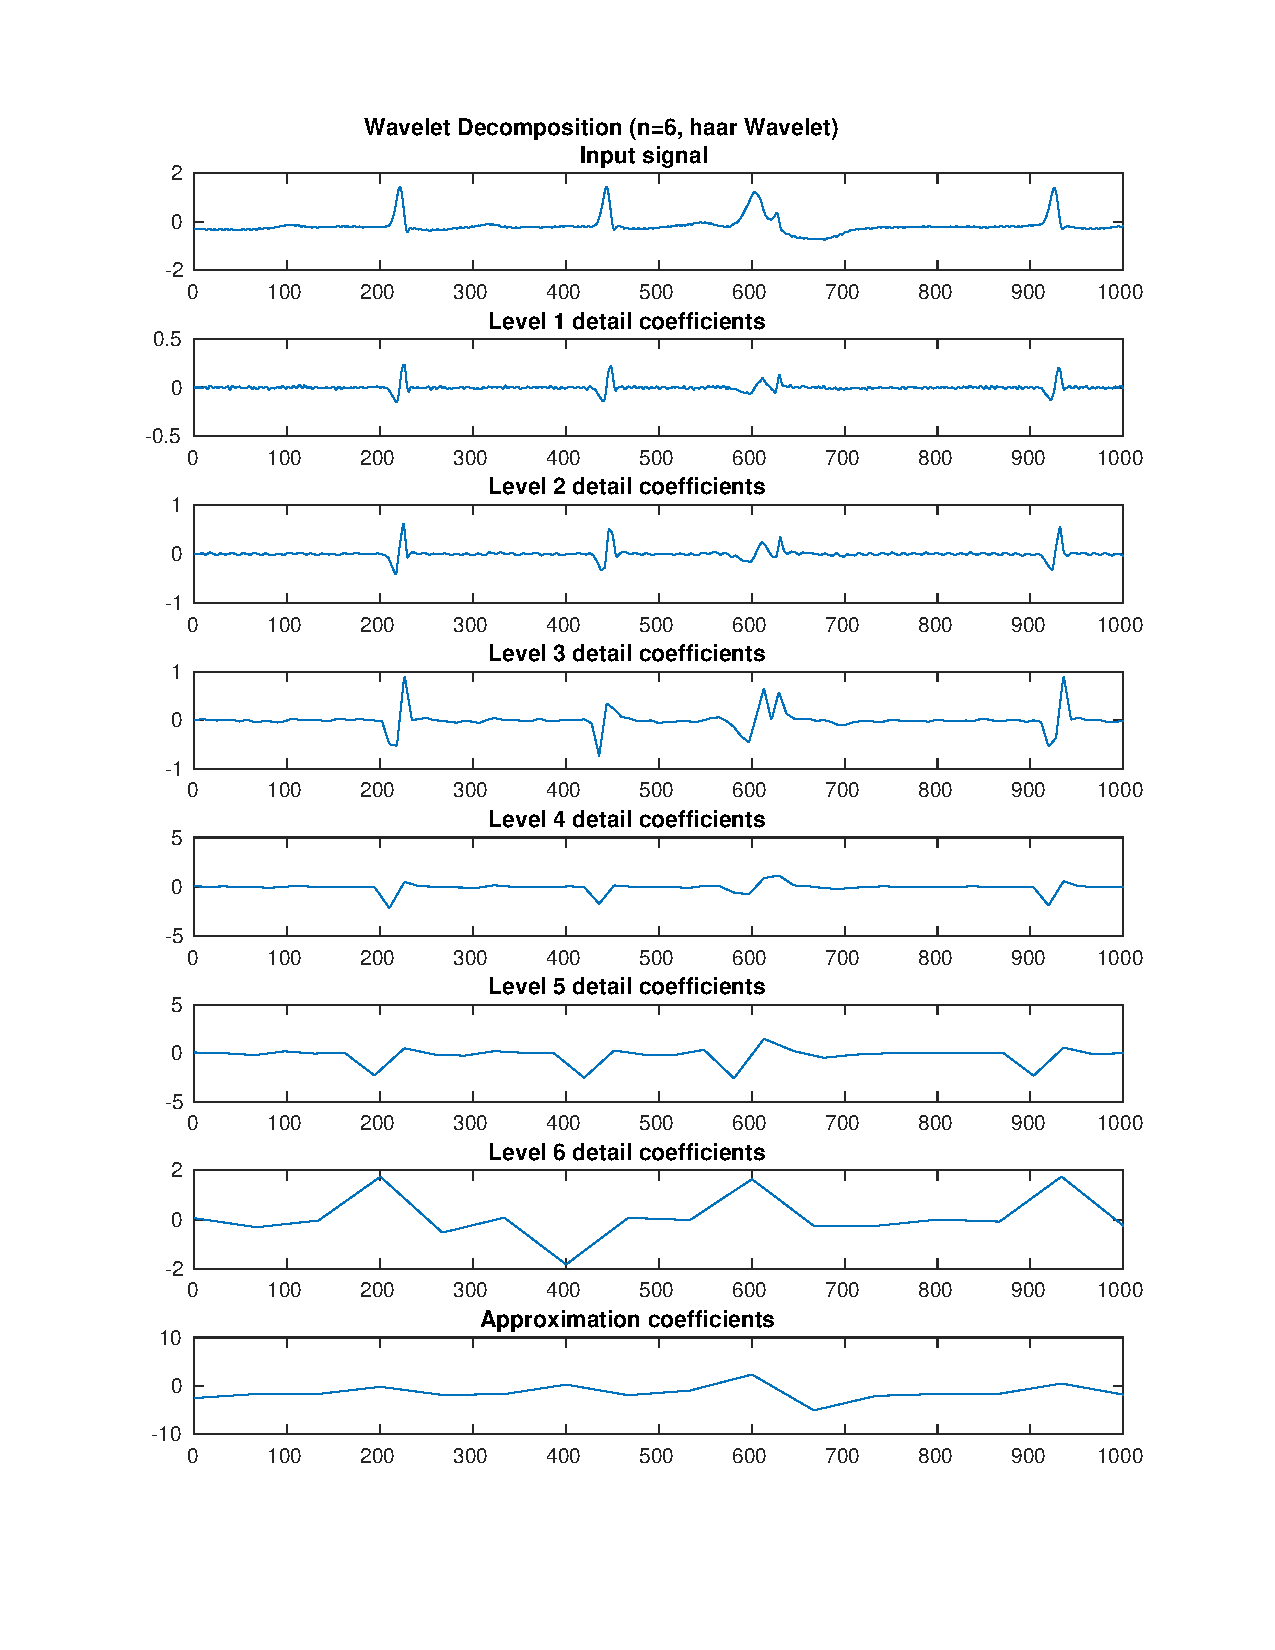
\includegraphics[width=\textwidth]{fig/221l1_dwt1.pdf}
\end{minipage}
\begin{minipage}{0.48\textwidth}
	\centering
	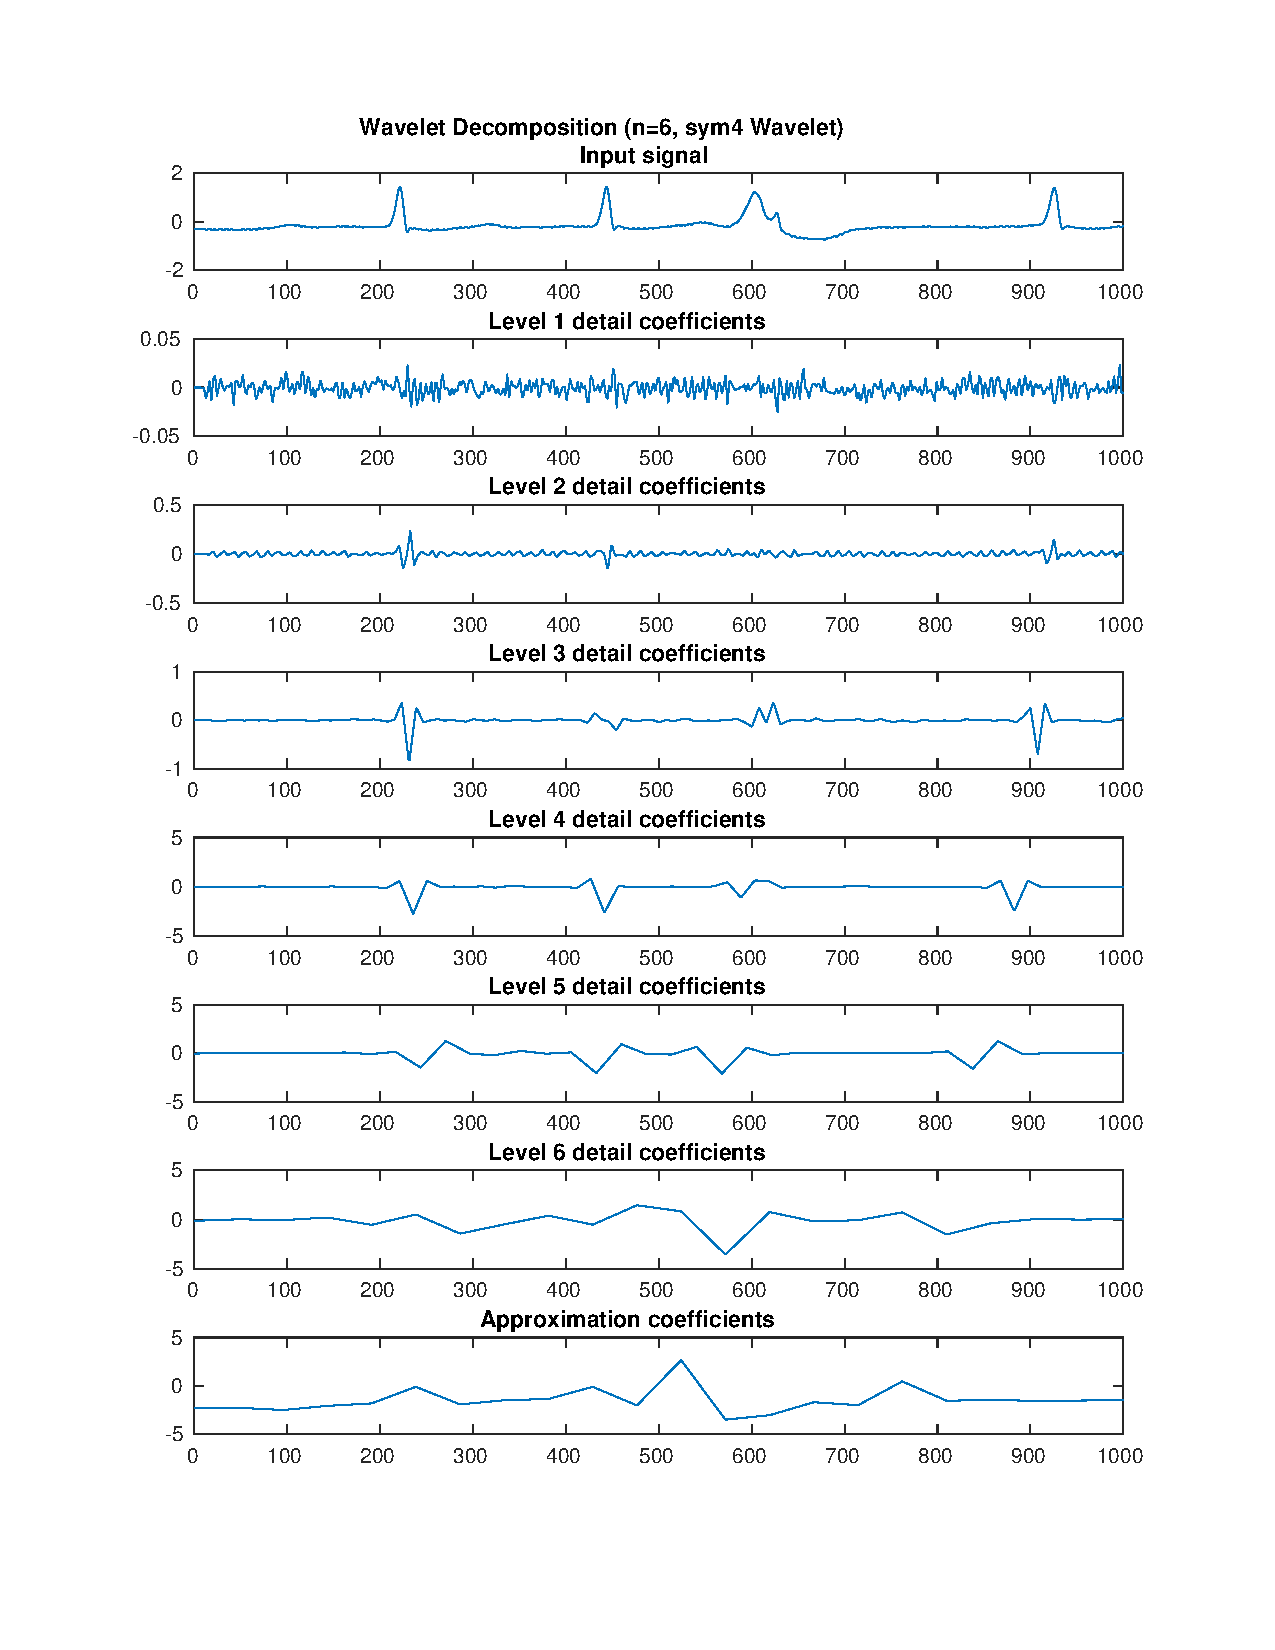
\includegraphics[width=\textwidth]{fig/221l1_dwt2.pdf}
\end{minipage}
\vfill
\caption{Διακριτός WT του σήματος χρησιμοποιώντας db4 και bior1.3.}
\label{fig:221l1_dwt}
\end{figure}


% --- EMD/HHT ---
\begin{figure}[H]
\centering
\begin{minipage}{0.48\textwidth}
	\centering
	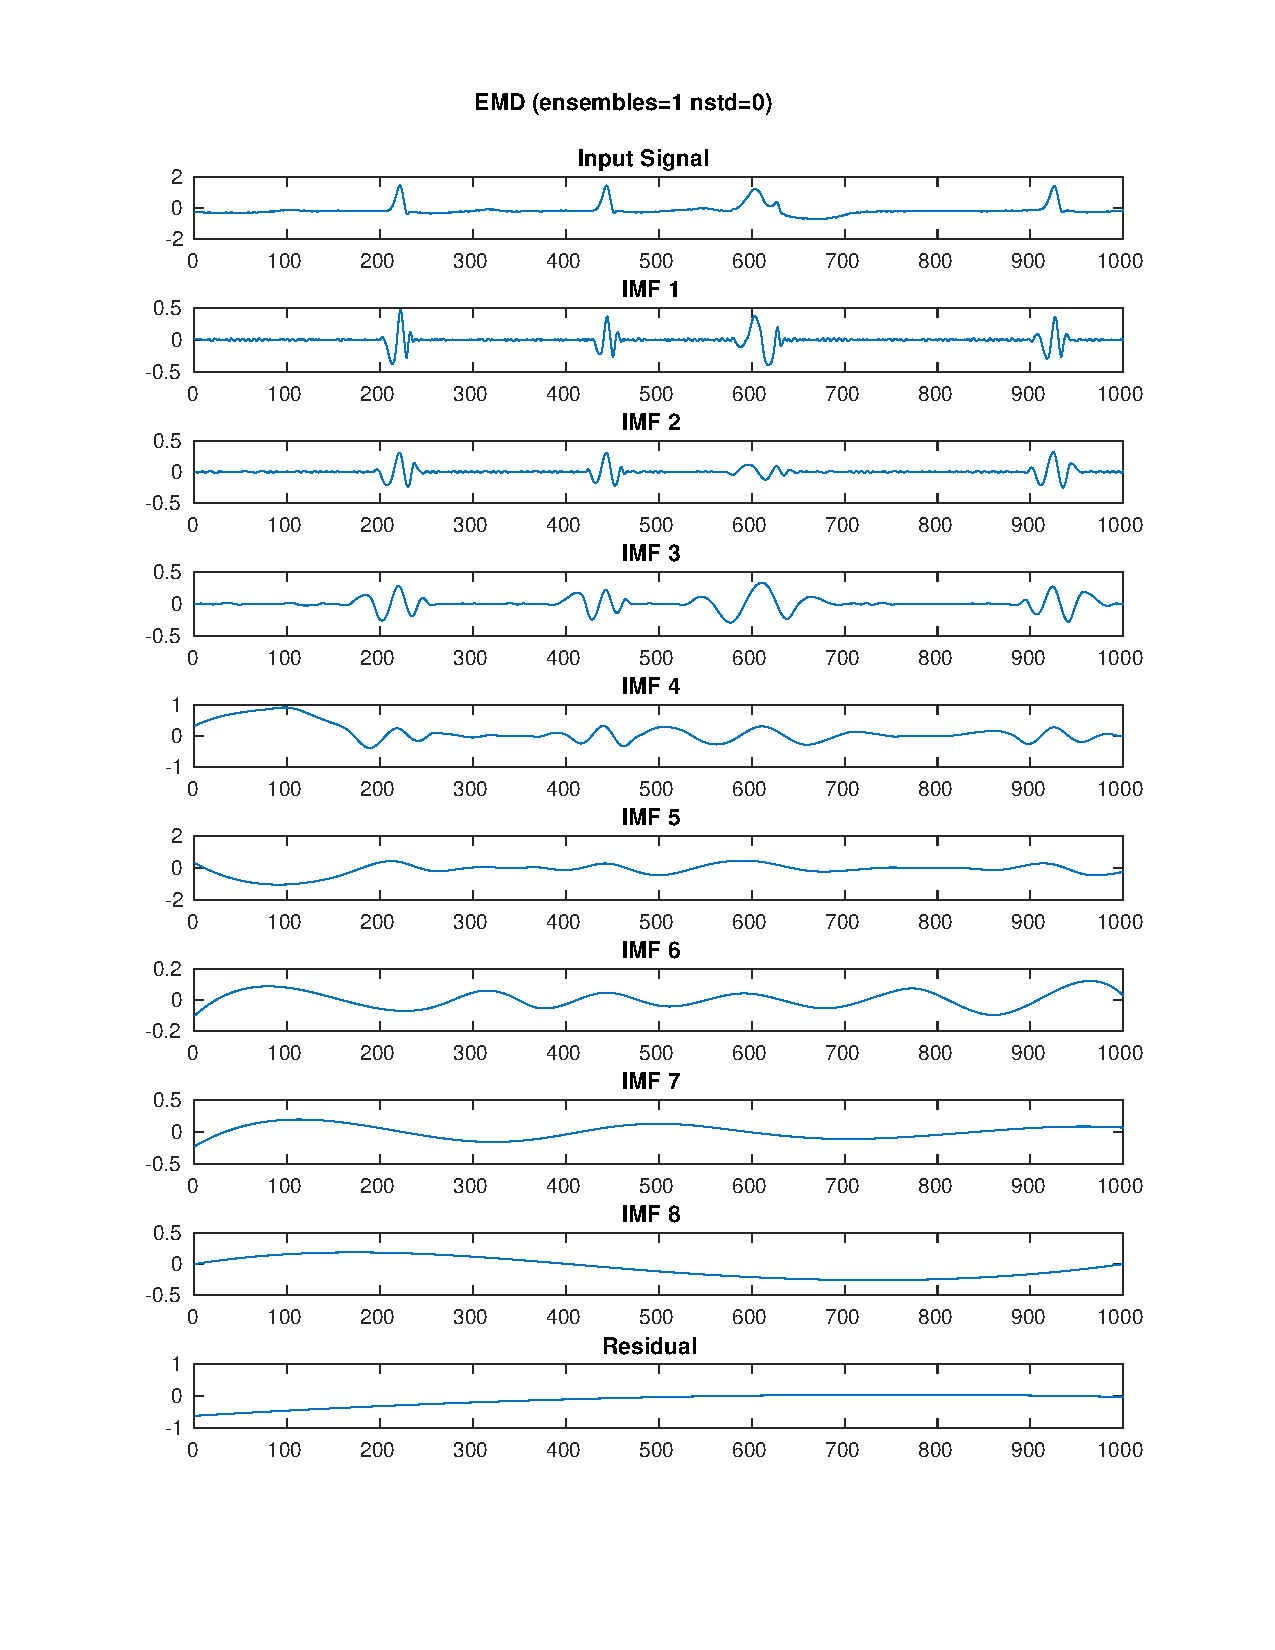
\includegraphics[width=\textwidth]{fig/221l1_emd.pdf}
\end{minipage}
\begin{minipage}{0.48\textwidth}
	\centering
	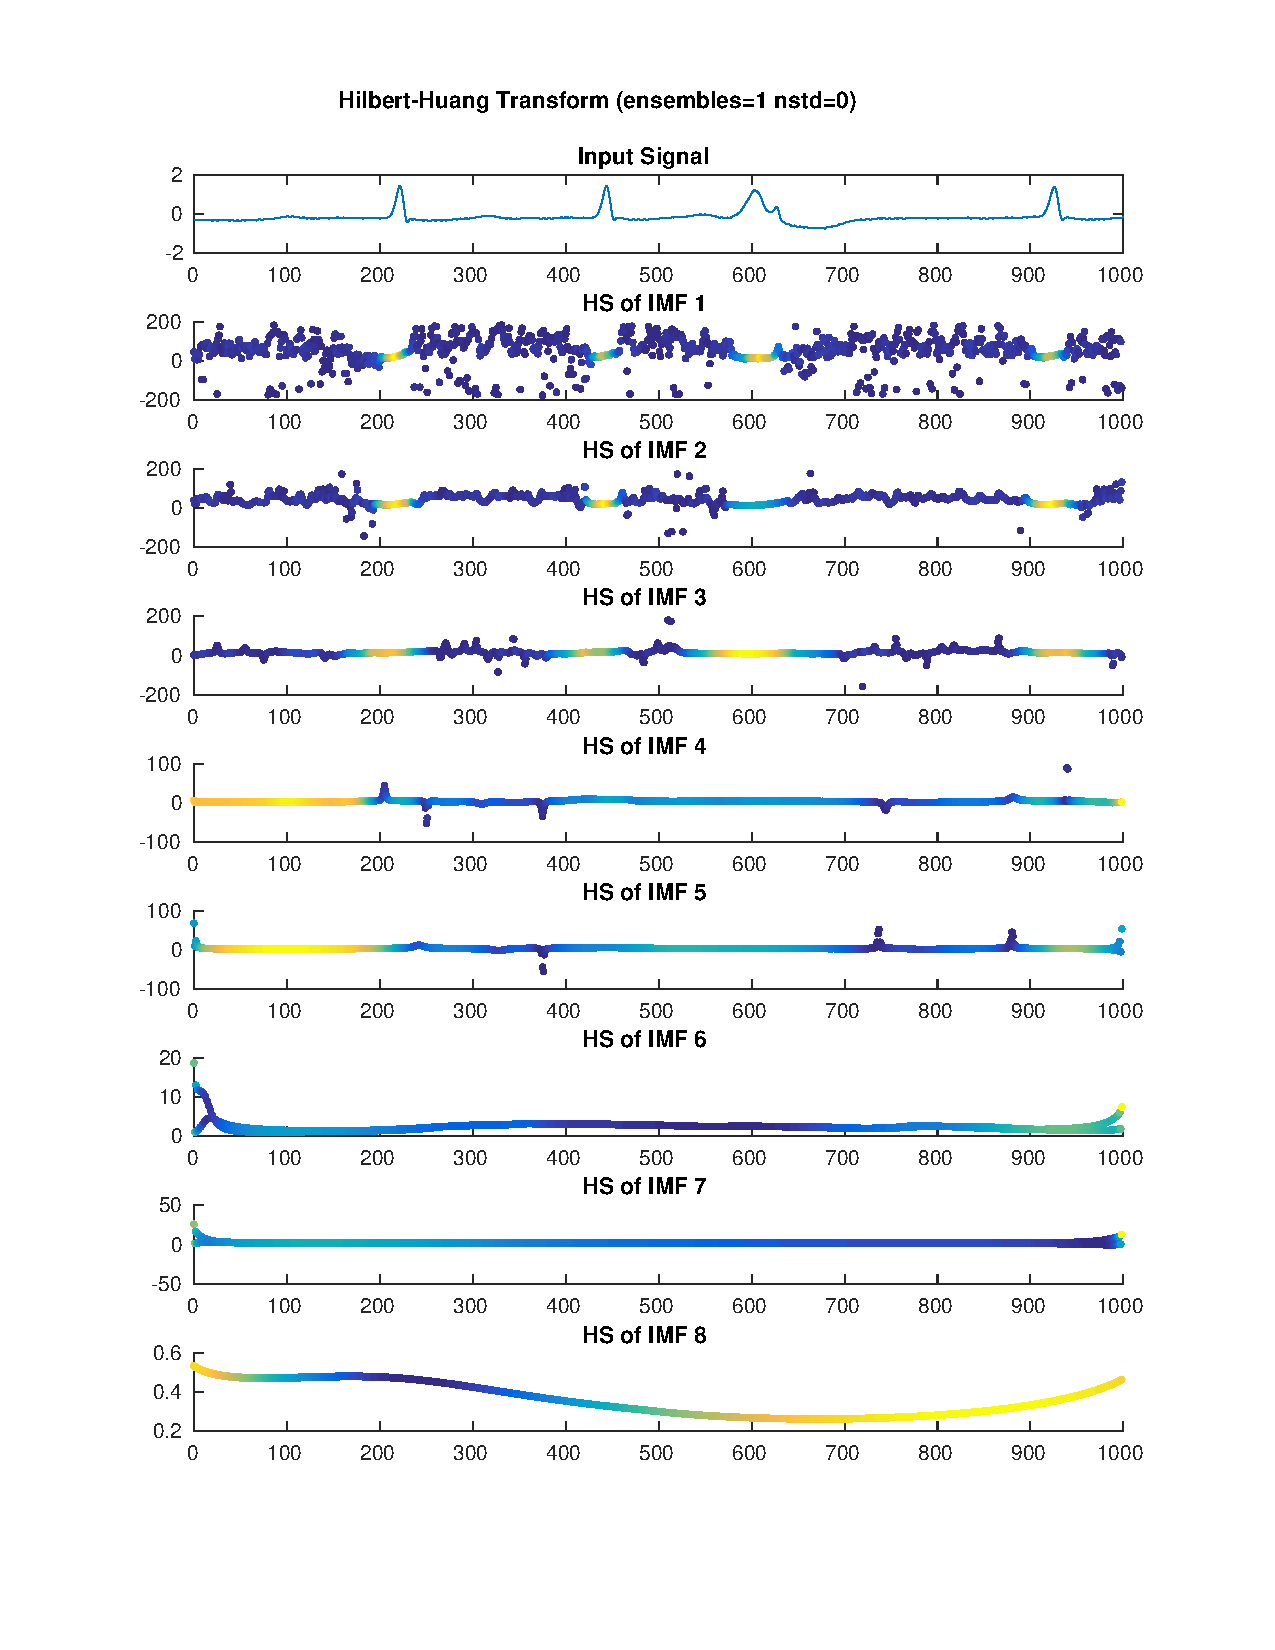
\includegraphics[width=\textwidth]{fig/221l1_hht.pdf}
\end{minipage}
\vfill
\caption{EMD και HHT του σήματος.}
\label{fig:221l1_hht}
\end{figure}


% --- EEMD/HHT ---
\begin{figure}[H]
\centering
\begin{minipage}{0.48\textwidth}
	\centering
	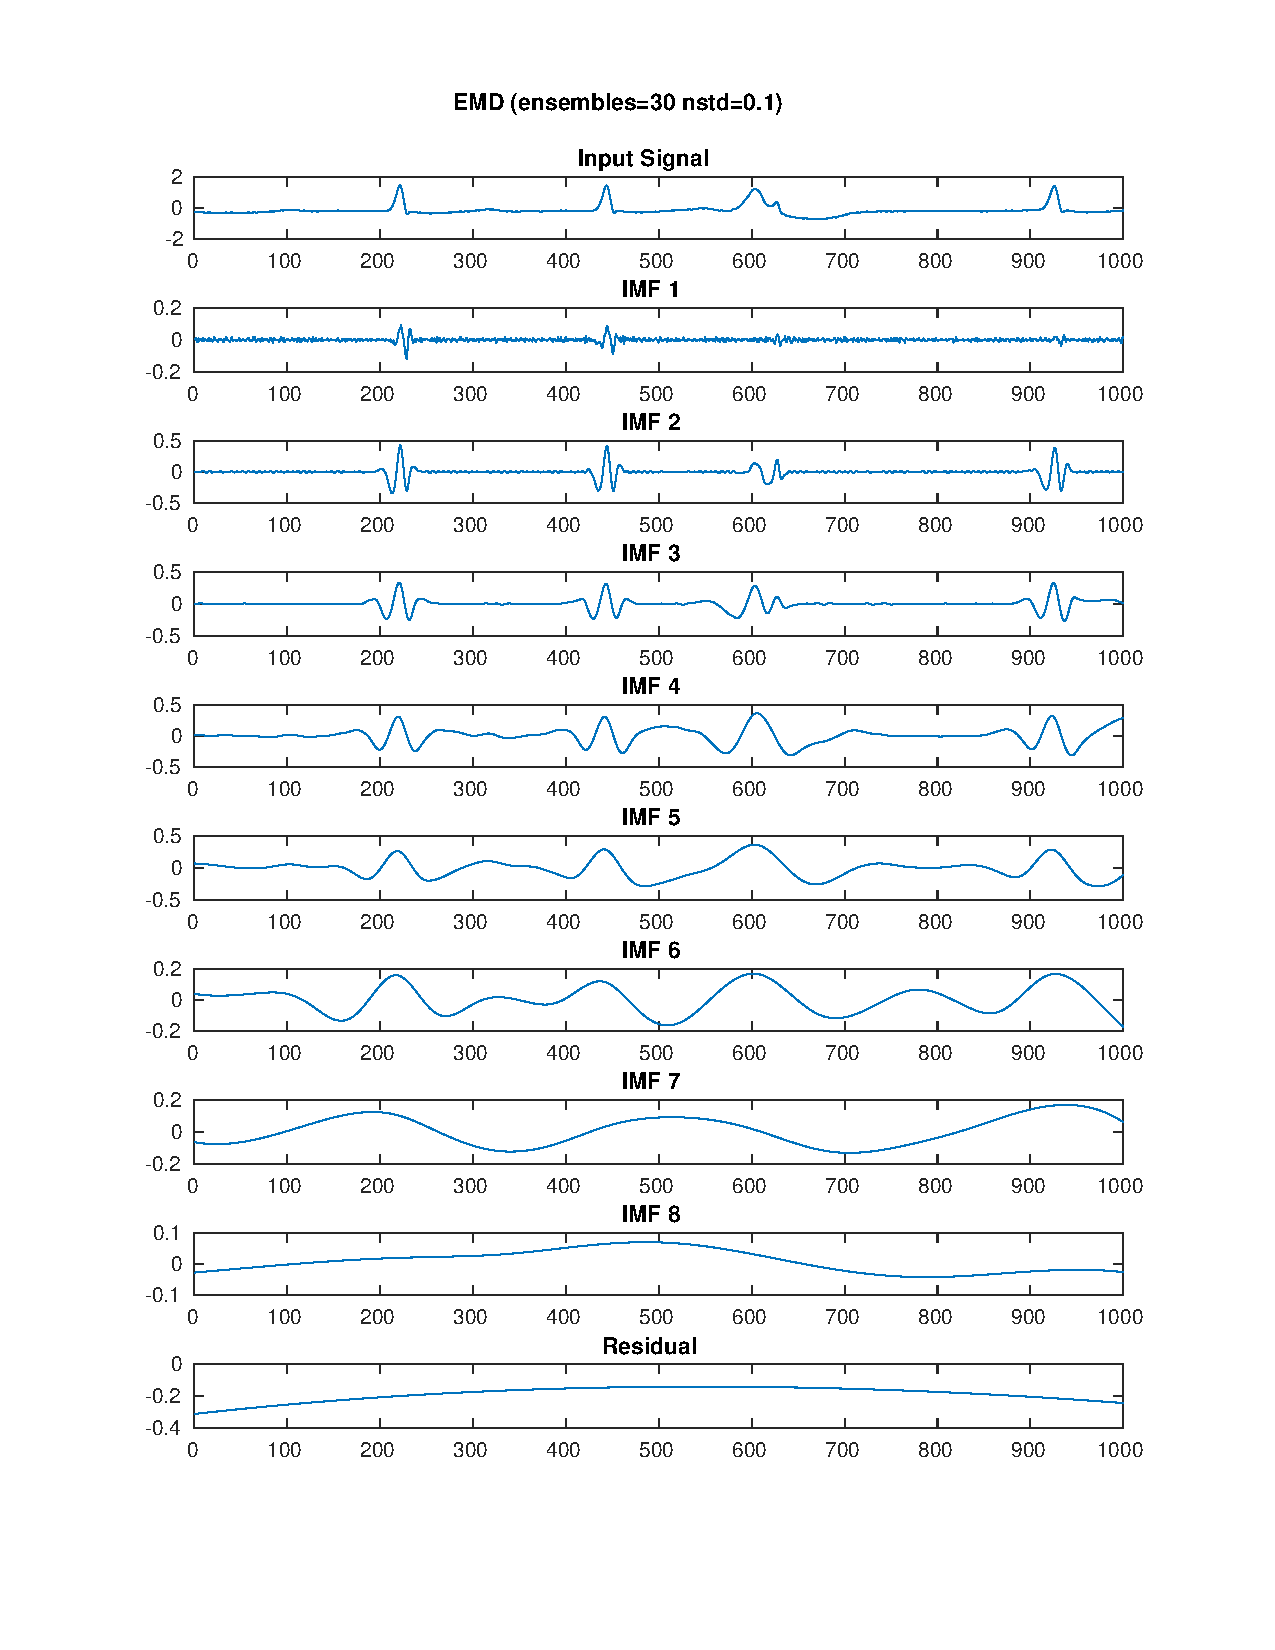
\includegraphics[width=\textwidth]{fig/221l1_emd_ensemble.pdf}
\end{minipage}
\begin{minipage}{0.48\textwidth}
	\centering
	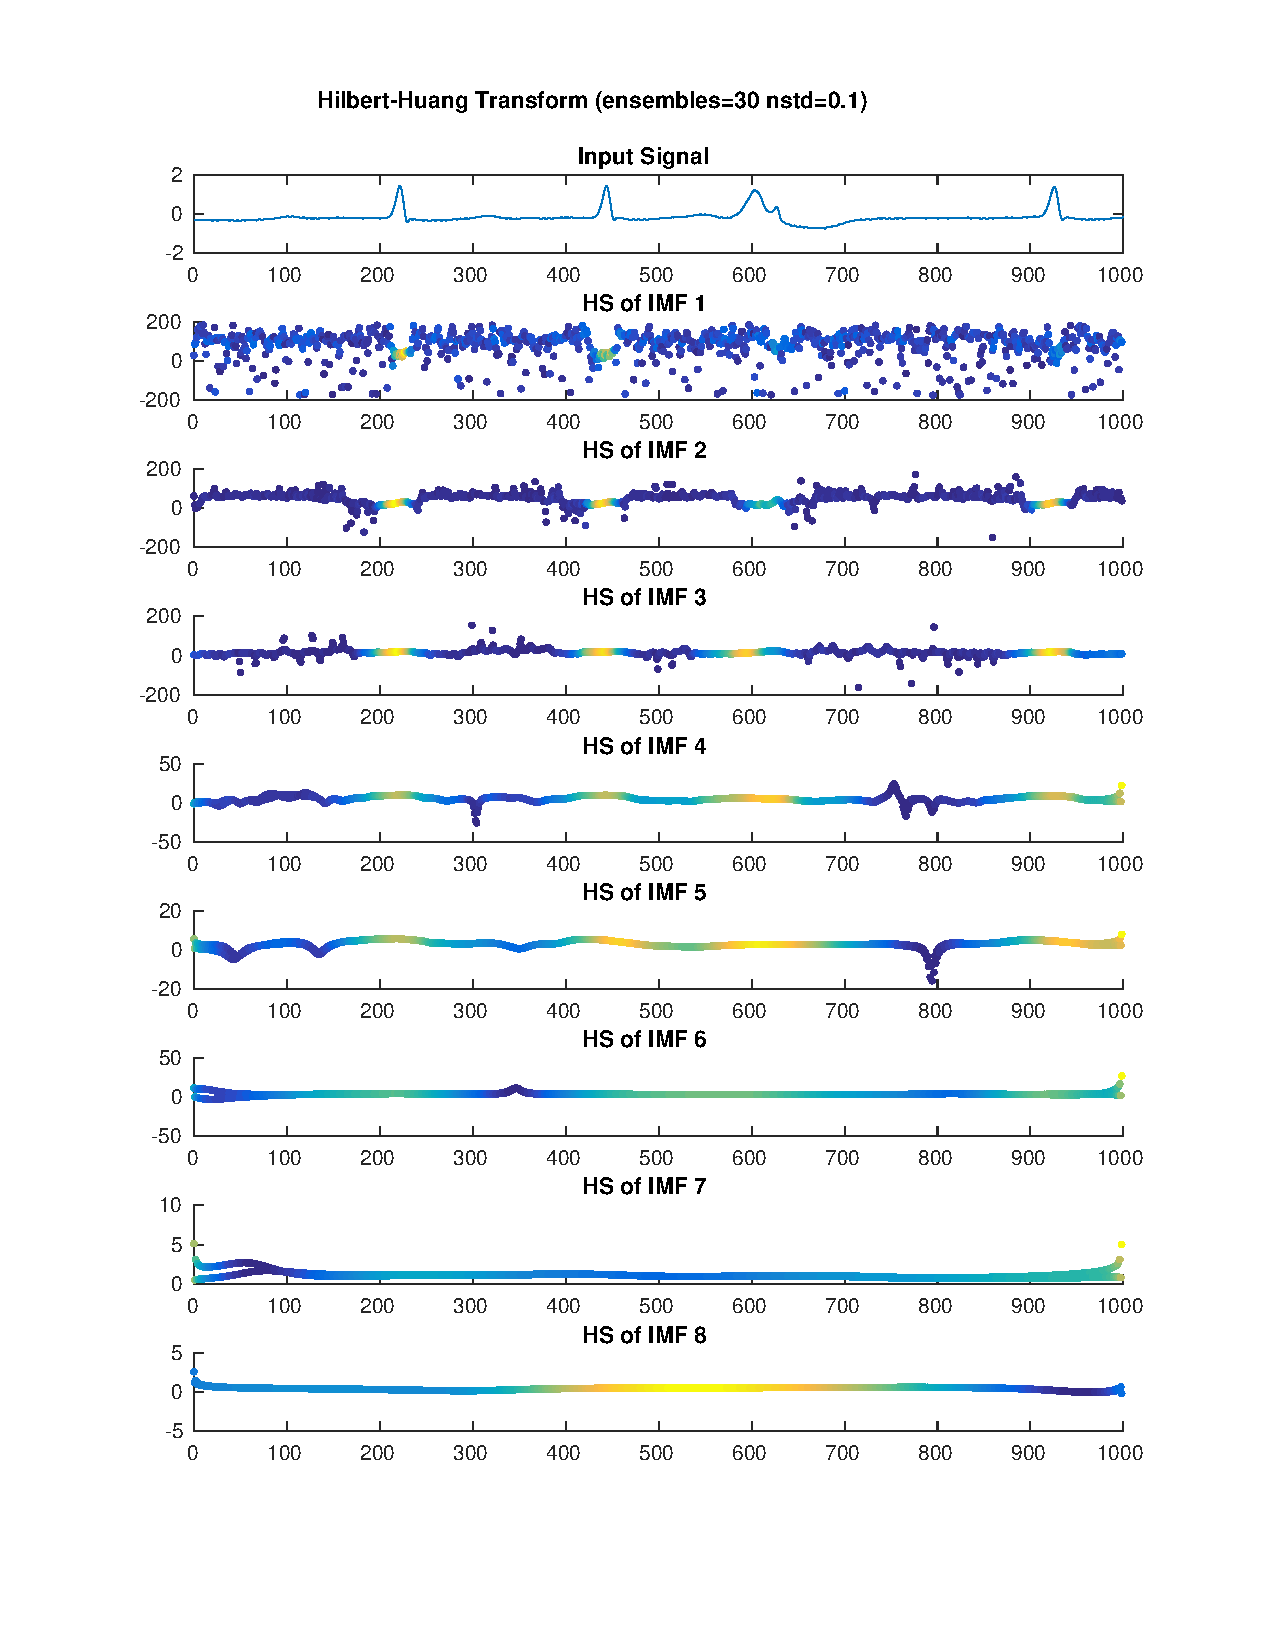
\includegraphics[width=\textwidth]{fig/221l1_hht_ensemble.pdf}
\end{minipage}
\vfill
\caption{EEMD και HHT με $n_{ens}=100$ και $\sigma_n = 0.1$.}
\label{fig:221l1_hht_ensemble}
\end{figure}

\section*{Ανίχνευση διαστημάτων R-R}

Ο αλγόριθμος που κατασκευάσαμε για την ανίχνευση των διαστημάτων R-R είναι ο εξής


\end{document}